% -*- Mode:TeX -*-

%% The documentclass options along with the pagestyle can be used to generate
%% a technical report, a draft copy, or a regular thesis.  You may need to
%% re-specify the pagestyle after you \include  cover.tex.  For more
%% information, see the first few lines of mitthesis.cls. 

\documentclass[12pt,vi,twoside]{mitthesis}

\usepackage[pdftex]{graphicx}

\usepackage{amsmath,amssymb,lgrind,wasysym}
% Some PDFtex-specific options
\usepackage[colorlinks=true,pdfstartview=FitV,linkcolor=blue,
            citecolor=magenta,urlcolor=red]{hyperref}
\pagestyle{plain}
\bibliographystyle{unsrt}


% This section specifies what .tex files are included
\begin{document}

% -*-latex-*-
%
%---------  COVER PAGE
%  --------     &
% -----  ACKNOWLEDGEMENTS
%

\title{Sensitivity and Noise Analysis of 4 km Laser Interferometric Gravitational Wave Antennae}

\author{Rana Adhikari}
\department{Department of Physics}

\degree{Doctor of Philosophy}
\degreemonth{July}
\degreeyear{2004}
\thesisdate{July 7, 2004}

%% By default, the thesis will be copyrighted to MIT.  If you need to copyright
%% the thesis to yourself, just specify the `vi' documentclass option.  If for
%% some reason you want to exactly specify the copyright notice text, you can
%% use the \copyrightnoticetext command.  
%\copyrightnoticetext{\copyright IBM, 1990.  Do not open till Xmas.}

% If there is more than one supervisor, use the \supervisor command
% once for each.
\supervisor{Rainer Weiss}{Professor}
\supervisor[Thesis Co-Supervisor]{Peter Fritschel}{Principal Research Scientist}
%\supervisor{Peter Fritschel}{Research Scientist}

% This is the department committee chairman, not the thesis committee
% chairman.  You should replace this with your Department's Committee
% Chairman. Except for in the physics department where we use
% Greytak apparently
\chairman{Thomas J. Greytak}{Associate Department Head for Education}

% Make the titlepage based on the above information.  If you need
% something special and can't use the standard form, you can specify
% the exact text of the titlepage yourself.  Put it in a titlepage
% environment and leave blank lines where you want vertical space.
% The spaces will be adjusted to fill the entire page.  The dotted
% lines for the signatures are made with the \signature command.
\maketitle

% The abstractpage environment sets up everything on the page except
% the text itself.  The title and other header material are put at the
% top of the page, and the supervisors are listed at the bottom.  A
% new page is begun both before and after.  Of course, an abstract may
% be more than one page itself.  If you need more control over the
% format of the page, you can use the abstract environment, which puts
% the word "Abstract" at the beginning and single spaces its text.

%% You can either \input (*not* \include) your abstract file, or you can put
%% the text of the abstract directly between the \begin{abstractpage} and
%% \end{abstractpage} commands.

% First copy: start a new page, and save the page number.
\cleardoublepage
% Uncomment the next line if you do NOT want a page number on your
% abstract and acknowledgments pages.
\pagestyle{empty}
\setcounter{savepage}{\thepage}
\begin{abstractpage}
% $Log: abstract.tex,v $
%             
%              ABSTRACT
% 
%

Around the world, efforts are underway to commission several kilometer-scale 
laser interferometers to detect gravitational radiation. In the United States,
there are two collocated interferometers in Hanford, Washington and one interferometer
in Livingston, Louisiana. Together, these three interferometers form the Laser
Interferometric Gravitational-wave Observatory (LIGO). 

The core of the work described in this thesis is the modeling and reduction of
the noise in the interferometers which limits their ultimate sensitivity.

A vital component of the noise reduction is the modeling, design, and implementation
of $\sim$100 feedback control systems. The most critical of these systems
are described and motivated.

Although improvements are continuously being made to the stability and noise character
of these detectors, several months of data have been collected. Various efforts
are underway to search through these data for gravitational wave signals.
Included here, is a description of a search made through the data for signals
from the ringdown of the quasi-normal modes of Kerr black holes.

In addition, several possible future improvements to the detectors are outlined.

\end{abstractpage}

% Additional copy: start a new page, and reset the page number.  This way,
% the second copy of the abstract is not counted as separate pages.
% Uncomment the next 6 lines if you need two copies of the abstract
% page.
% \setcounter{page}{\thesavepage}
% \begin{abstractpage}
% % $Log: abstract.tex,v $
%             
%              ABSTRACT
% 
%

Around the world, efforts are underway to commission several kilometer-scale 
laser interferometers to detect gravitational radiation. In the United States,
there are two collocated interferometers in Hanford, Washington and one interferometer
in Livingston, Louisiana. Together, these three interferometers form the Laser
Interferometric Gravitational-wave Observatory (LIGO). 

The core of the work described in this thesis is the modeling and reduction of
the noise in the interferometers which limits their ultimate sensitivity.

A vital component of the noise reduction is the modeling, design, and implementation
of $\sim$100 feedback control systems. The most critical of these systems
are described and motivated.

Although improvements are continuously being made to the stability and noise character
of these detectors, several months of data have been collected. Various efforts
are underway to search through these data for gravitational wave signals.
Included here, is a description of a search made through the data for signals
from the ringdown of the quasi-normal modes of Kerr black holes.

In addition, several possible future improvements to the detectors are outlined.

% \end{abstractpage}

\cleardoublepage

\section*{Acknowledgments}

I have had the uncommon luck of working with many people in the project.
Its probably true that I've learned something from each and so a complete
list of people I would thank would make this thesis so thick that even
fewer people would read it. Instead I will just thank the people who
have given me the most work to do.

To Mike, thanks for teaching me how to drag wipe optics and how 
to calibrate a scope probe. Thanks for yelling at me if I (or any other grad
student) made a mess in the machine shop. Thanks for all the free food
and for taking that lemon off of my hands.

To Peter, thanks for putting up with all of those bad measurements,
ideas, and electronics. And for that timely invitation to
help out with that 15 meter cavity.

To Rai, thanks for hiring me. This is the longest I've ever held a job.
Thank you for letting me practice with one of your interferometers for a
few years. And most of all for being an example of the integrity and the
passion with which science should be done.

-

- Rana \today
%%%%%%%%%%%%%%%%%%%%%%%%%%%%%%%%%%%%%%%%%%%%%%%%%%%%%%%%%%%%%%%%%%%%%%
% -*-latex-*-

\pagestyle{plain}
  % -*- Mode:TeX -*-
%% This file simply contains the commands that actually generate the table of
%% contents and lists of figures and tables.  You can omit any or all of
%% these files by simply taking out the appropriate command.  For more
%% information on these files, see appendix C.3.3 of the LaTeX manual. 
\tableofcontents
%\newpage
\listoffigures
%\newpage
\listoftables


%
%
%     INTRODUCTION
%
%
%------------------------------------------------------------------------------
\chapter*{Introduction}
\addcontentsline{toc}{chapter}{Introduction}

A handful of kilometer scale, laser interferometers have begun operation in the
last few years with the goal of detecting gravitational waves.
They are all steadily approaching their designed sensitivities, alternating data 
taking runs with further detector improvements.
This worldwide network of observatories includes the German-British 
GEO600~\footnote{
\href{http://www.geo600.uni-hannover.de}{http://www.geo600.uni-hannover.de}}
~\cite{GEO:StatusCQG}, 
the Japanese TAMA~\footnote{
\href{http://tamago.mtk.nao.ac.jp}{http://tamago.mtk.nao.ac.jp}}\cite{TAMA:StatusCQG},
and a set of 3 interferometers in the United States called 
LIGO~\footnote{
\href{http://ligo.caltech.edu}{http://ligo.caltech.edu}}
~\cite{LIGO:StatusCQG,Rai:PhysicsToday}. 
Also expected to come on-line in the near future is the Italian-French
VIRGO~\footnote{
\href{http://www.virgo.infn.it}{http://www.virgo.infn.it}}~\cite{VIRGO:StatusCQG}.
% and 
%the Australian AIGO~\footnote{
%\href{http://www.anu.edu.au/Physics/ACIGA}{http://www.anu.edu.au/Physics/ACIGA}}
%~\cite{ACIGA:StatusCQG}. 
All of these
observatories employ (or will employ) enhanced Michelson interferometers illuminated 
by highly stabilized, medium power lasers operating at 1064~nm. All of the 
interferometers' optics are suspended by seismic isolation systems and 
are housed in high to ultra-high vacuum beamtubes.

This thesis only describes the LIGO detectors, concentrating on the
Louisiana 4 km interferometer.

Chapter~\ref{chap:GW} describes briefly the generation of gravitational waves,
speculations on possible sources, and their detectability based on a theoretical
noise estimate of the interferometers.

Chapter~\ref{chap:IFO} motivates the design of the power recycled, 
Fabry-Perot Michelson interferometer configuration used in LIGO.

Chapter~\ref{chap:signals} describes the scheme
used to readout the signals conatining information about the interferometer
lengths and also the gravitational wave signal.

Chapter~\ref{chap:noise} lists all of the significant noise sources, their
coupling mechanisms, and makes estimates for their contribution to the total
noise budget. This chapter and the following one are the core of the thesis.

Chapter~\ref{chap:controls} discusses the control systems, mainly focusing
on the length controls: the motivation for controls, the troubles with their noise,
and some transfer functions of control loops. 

Chapter~\ref{chap:ringdowns} describes a search made through the data for
damped sinusoid signals.

Chapter~\ref{chap:future} gives examples of work that can be done on these first
generation of interferometers to dramatically increase the event rate. 

The Appendices provides some further details on topics which are briefly mentioned 
in the main text.


This work, and the LIGO Laboratory, is supported by the National 
Science Foundation\footnote{\href{http://www.nsf.gov/}{http://www.nsf.gov/}}, 
grant PHY-0107417.

%---   CHAPTER 1          - ---- ---- -- -----------------

%---      GRAVITY WAVES           --------------------------
%

\chapter{Gravitational Radiation}
\label{chap:GW}

\begin{figure}[!h]
\centerline{\includegraphics[angle=0,width=6.5in]{Figures/Chap1/GRB-DestroyStar.jpg}}
\end{figure}
\clearpage

This chapter describes gravitational waves and their possible sources.

Section~\ref{sec:GR} describes the concept of gravitational waves and the space-time
strain which we expect to measure in the far-field of a radiator.

Section~\ref{sec:Sources} discusses 4 different classes of signals and is a review
of current source strength and rate estimates.

%Section~\ref{sec:Searches} lists selected gravitational wave searches done in the
%past and tabulates the resulting upper limits.


%------------------------------------------------------------------------------
\section{Gravitational Radiation in General Relativity}
\label{sec:GR}

%In Special Relativity, the laws of physics are the same to observers in
%different inertial reference frames. The space-time interval between events
%is invariant among these reference frames. The interval is defined as:

%\begin{equation}
%ds^2 \equiv -c^2 dt^2 + dx^2 + dy^2 + dz^2 \equiv  \eta_{\mu \nu} dx^{\mu} dx^{\nu} 
%\label{eq:special}
%\end{equation}

%Here the $\eta$ tensor defines the Minkowski metric.

The theory of General Relativity~\cite{Einstein:Book} describes gravity as a 
consequence of the curvature of space and time (or space-time). One of the
predictions of the theory is gravitational radiation from fluctuating
mass-energy distributions~\cite{MTW}. Although these ripples can, 
in principle, severely distort the space and time very near the radiator,
far from the source one can express the effect of these waves as small
perturbations to the otherwise flat space-time background. In this weak field limit
the space-time metric can be approximated as

\begin{equation}
g_{\mu \nu} \simeq \eta_{\mu \nu} + h_{\mu \nu}, 
                  \quad \mbox{where} \quad   |h_{\mu \nu}| \ll 1
\label{eq:gmunu}
\end{equation}
and where $\eta_{\mu \nu}$ is the Minkowski metric representing flat space and 
$h_{\mu \nu}$ is the perturbation to flat space due to the gravity wave.

By an adept coordinate transform~\cite{MTW} the gravitational wave may be written as:

\begin{equation}
h_{\mu \nu}(z,t) = 
\left(
\begin{matrix}
0    & 0        & 0          & 0 \\
0    & -h_{+}    &  h_{\times}     & 0 \\
0    & h_{\times}    & h_{+}     & 0 \\
0    & 0        & 0          & 0 
\end{matrix} 
\right) 
\cos{\omega \left( \frac{z}{c}- t \right)}
\label{eq:hmatrix}
\end{equation}
where $\omega$ is the gravitational wave frequency and the two independent 
polarizations are $h_{+}$ and $h_{\times}$.



\subsection{Measurable Effect on Free Masses}

From an observers point of view, we can ask about what the measurable effects are
of gravitational waves. To answer this we set up two free masses, one located at
the origin and one located a distance, $x = L$, from the origin. We can measure the
separation between these two masses by sending a plane wave of light from the origin
to bounce off of the far mass and measure the phase of the return wave.
The accrued round trip phase is:

\begin{equation}
\Phi_{rt}(t_{rt}) = \int\limits_{0}^{t_{rt}} 2 \pi f \, dt
\label{eq:roundtripflat}
\end{equation}
where $t_{rt}$ is the time it takes for the light to make one round trip and
$f$ is the frequency of the light. In the absence of radiation, we can do the
integral by changing it into an integral over length. To do this we use the 
flat space metric, $\eta_{\mu \nu}$, to relate space and time for light
($t_{rt} = 2 L/c$ and $dt = dx / c$). 

In the presence of a gravitational wave, we instead use Equation~\ref{eq:gmunu} to calculate
the space-time interval so now the round trip phase is

\begin{equation}
\Phi_{rt}(t_{rt}) = 2 \frac{2 \pi f}{c} \int\limits_{0}^{L} \sqrt{|g_{xx}|} \, dx
                    \simeq 2 (1 - h_{+}/2) \frac{2 \pi L}{\lambda}
\label{eq:roundtrip}
\end{equation}
in the case of a ''plus'' oriented wave with a period much longer than the round trip
light travel time. Repeating this integral, but doing the
integration now along the y-axis, we get that 
$\Phi_{rt} \simeq 2 (1 + h_{+}/2) (2 \pi L / \lambda)$. The difference
in the phase shift between the two arms gives 
$\Delta \Phi \simeq 2 h_{+} (2 \pi L / \lambda)$. 

Interpreting the phase shifts as length measurements indicates that the apparent 
length of each arm is stretched and compressed as the gravity wave passes. 
A diagram of this is shown in Figure~\ref{fig:CropCircles}. The
length shift is proportional to the original distance between the masses,

\begin{equation}
\frac{\Delta L}{L} = \frac{1}{2} h_+
\label{eq:h}
\end{equation}
which is why a gravitational wave is usually said to cause a strain in space.


\begin{figure}[!h]
\centerline{\includegraphics[angle=0,width=6.5in]{Figures/Chap1/CropCircles.png}}
\caption[Effect of gravitational waves on Test particles]{Shown are the effects of $+$ and
         $\times$ waves propagating in the z direction on a circle of test particles
         in the x-y plane.}
\label{fig:CropCircles}
\end{figure}


\subsection{Radiation Amplitudes}

Conservation of mass-energy, linear momentum, and angular momentum rule out 
monopole, dipole, and ''magnetic'' dipole radiation, respectively. With no
conservation law to rule it out, the leading term in gravitational
radiation is the oscillating quadrupole mass-energy distribution. In
addition, for the wave to carry away energy from the source, the amplitude
of the wave must decay as $\sim 1/r$.

A rough estimate for the strain amplitude is\cite{Kip:300}:

\begin{equation}
\begin{aligned}
h &\sim \frac{G}{c^4}\frac{\ddot{Q}}{r} \\
  &\sim \frac{G}{c^4}\frac{E_{kin}^{ns}}{r} \\
  &\sim 10^{-19} \left(\frac{E_{kin}^{ns}}{M_{\astrosun} c^2}\right)
                    \left(\frac{1 \, \mbox{Mpc}}{r}\right)
\end{aligned}
\label{eq:h_estimate}
\end{equation}
using the estimate that the non-spherical kinetic energy, $E_{kin}^{ns}$,
contributing to gravitational radiation is roughly equal to the second
time derivative of the quadrupole moment, $\ddot{Q}$. This is a very
optimistic estimate assuming a huge amount of energy is converted into
gravitational waves in a neighboring galaxy. However,
it indicates an upper limit to expected signal strengths. 

The radiated energy (luminosity) is related to the strain by~\cite{Landau:Fields}:

\begin{equation}
\begin{aligned}
\frac{dE_{\mbox{\tiny GW}}}{dt} &= \frac{c^3 r^2}{4 \, G} 
                      (\dot{h_{+}^2} + \dot{h_{\times}^2}) \\
                   &\simeq 10^{34} \left(\frac{r}{1 \, \mbox{Mpc}}\right)^2
                                   \left(\frac{|h|}{10^{-23}}\right)^2 
                     \mbox{Watts}
\label{eq:Luminosity}
\end{aligned}
\end{equation}
This estimate gives a very small measurable strain, even though the radiated
energy is quite large; space-time is a very 'stiff' wave medium.


%------------------------------------------------------------------------------
\section{Astrophysical Sources}
\label{sec:Sources}

The following sections briefly describe some types of gravitational wave
sources and their predicted strengths, frequencies, and detection rates. 
A more extensive survey can be found in Refs.~\cite{Kip:300,Kip:Probing}

Later in the thesis (Chapter~\ref{chap:ringdowns}), a search for ringdowns of
black hole quasi-normal modes is described. To accompany that work, the end of 
this chapter describes the generation of ringdown signals.


\subsection{Monochromatic Signals}

\begin{figure}[!h]
\centerline{\includegraphics[angle=0,width=6.5in]{Figures/Chap1/pulsars.pdf}}
\caption[Known Pulsars]{Upper limits on the amplitudes of many known
         pulsars compared to the upper limit set by each 
         interferometer separately during the second LIGO science run (S2). The pulsar 
         amplitude limits are made by assuming that all of the
         rotational energy loss of the pulsar goes into gravitational radiation.
         The 'SRD' curve is the LIGO Science Requirement for a 4 km interferometer
         after 1 year of integration.}
\label{fig:pulsars}
\end{figure}

One class of signal being searched for emits radiation at a single frequency,
producing a long continuous wave in the source's reference frame. 
The most commonly described
monochromatic  source is the radiation from a non-axisymmetric pulsar.
The time-dependent quadrupole moment necessary to generate gravitational waves
may come from a wobbling rotation (spin axis not aligned with a principle axis)
or a small deviation of the pulsar shape from perfect axial symmetry (a bump).
In the latter case the gravitational wave strain can be written as~\cite{Kip:300}

\begin{equation}
h \sim 2 \times 10^{-26} \left(\frac{f_{rot}}{1 \, \mbox{kHz}} \right)^2
             \left(\frac{10 \, \mbox{kpc}}{r} \right)
             \left(\frac{\epsilon}{10^{-6}} \right)
\end{equation}
where $f_{rot}$ is the frequency of rotation, $r$ is the
distance between the source and the detector, and 
$\epsilon \equiv (I_{xx}-I_{yy})/I_{zz}$, is the equatorial ellipticity.


It has been suggested~\cite{Bildsten:Braking} and somewhat supported by
observation~\cite{Deepto:Braking} that low-mass X-ray binaries (LMXBs) reach
an equilibrium where the spin-up torque due to accretion is balanced by the
spin-down from gravitational wave emission.

%The strong frequency dependence of the torque is apparently why the observed
%range of pulsar frequencies is so small (f $\approx$ 200-50 MHz crap).


\subsubsection{Upper Limits and Measurements}

Searches have been made for gravitational wave signals from pulsars; see for 
example~\cite{Hereld:Thesis,Mike:Thesis,S1:Pulsar} and references therein.

Figure~\ref{fig:pulsars} shows upper limits on the amplitudes of many known
pulsars compared to the upper limit set by each interferometer separately during
the S2 run. The amplitude of the dots are calculated by assuming that all of the
rotational energy loss of the pulsar, determined by measuring the spin-down
rate, goes into gravitational radiation.





\subsection{Stochastic Background}

Quite different in character from monochromatic sources is the
stochastic background of gravitational radiation~\cite{S1:Stochastic}.
A stochastic background can have both cosmological and
astrophysical sources such as amplification by inflation of zero-point 
metric fluctuations, phase transitions in the 
early universe, cosmic strings, and a large number of unresolved foreground
sources such as binaries and supernovae~\cite{Bruce:Houches}.

Schemes for detecting a stochastic background generally involve
cross-correlating the output of two or more 
detectors~\cite{Nelson:Thesis,Nelson:SB,Bruce:Houches,S1:Stochastic}. 
%The idea being that the there are no non-gravitational wave correlations
%among the detectors. 

The past and present analyses of a stochastic background have made some assumptions about
the statistical character of the signal: it is isotropic, unpolarized,
stationary, and Gaussian. These assumptions are discussed 
by Allen~\cite{Bruce:Stochastic};

See \cite{S1:Stochastic} for a review of current upper limits and
prospects for the future.



\subsection{Bursts}

A very large class of events are the unmodeled transients, or bursts. These
are searched for quite differently than most of the other types of signals
in this chapter. Most approaches involve looking for excess power in many
narrow bands.

Some examples of the anticipated types of burst events being searched for are
asymmetrical core collapse in supernovae, coalescence and merger of intermediate
mass black holes, and most interestingly, the unknown.


\subsubsection{Previous Searches}

A review of burst searches made with resonant bar detectors is described
elsewhere~\cite{Bars:Status,Tyson:1982}. Here I list past searches for
gravitational wave bursts using laser interferometers and the strain
amplitudes they were sensitive to:


\begin{itemize}

\item R. Forward \qquad Malibu, CA  \quad 1977  \quad h $>$ 10$^{-14}$ for 150 hours.

\item D. Dewey   \qquad MIT 1.5m \qquad 1985 \quad h $>$ 10$^{-13}$ 

\item Glasgow / Max Planck \qquad \quad 1989 \quad h $> 5 \times 10^{-16}$

\item LIGO/GEO S1 (Aug. 2002, 17 days) \quad  h $>$ 10$^{-18}$

\item LIGO/GEO S2 (Feb. 2003, 2 months) \quad  h $>$ 10$^{-19}$

\end{itemize}


\subsection{Binary Inspiral}

An extensively studied source of gravitational wave is the decaying orbit of
two compact objects, usually referred to as a binary inspiral. In the LIGO band,
these objects can be neutron stars and/or black holes (NS/NS, BH/NS, BH/BH).

The waveforms, from the NS/NS inspiral,
are believed to be sufficiently well modeled that one can search for these 
signals using a matched filter technique~\cite{Bruce:chisquare}. The BH/BH waveforms 
are much more difficult to calculate~\cite{BCV1} and there is not as much 
confidence in these waveforms. Nevertheless, a matched filter search for these 
signals is currently being pursued as well.

As the
orbit of the two bodies progresses in time, the orbital period and separation
decrease due to energy loss through gravitational radiation. As the orbital 
separation decreases, the amplitude and frequency of the signal increase until
the binary separation falls below the Innermost Stable Circular Orbit (ISCO)
and the two stars plunge together and merge.

Reconstructing the merger of two neutron stars or two black holes is a very
computationally intensive exercise and there are numerous, highly active
efforts to calculate these dynamics and the associated gravitational radiation
waveforms using fast supercomputers~\cite{Jorge:Numerical}.

\subsubsection{Rate Estimates}

The recent discovery of PSR J0737-3039~\cite{Parkes:Nature}, a highly relativistic 
binary pulsar,
increased the predicted rate of galactic NS/NS inspirals detectable by LIGO
from one every few decades to one every few years~\cite{Vicki:Rates}. 
Previous estimates of
merger rates were dominated by the parameters of the famous 
PSR B1913+16 \cite{Hulse:Pulsar,Taylor:1913}. This new binary (actually the
first detected double pulsar system) has a 3X shorter coalescence time and
a 7X smaller luminosity. These factors have radically changed the population
and merger rate estimates for NS/NS binaries in the galaxy.

Although, at the time of this writing, there have been 
7 double neutron star systems discovered~\cite{Taylor:1829}, the 
detection rate estimates for LIGO are 
still precariously dependent on the tightest, darkest binary.


\subsubsection{Upper Limits and Measurements}

A few searches have been made so far for the signatures from NS/NS inspiral
events~\cite{S1:Inspiral,40m:Inspiral,TAMA:Inspiral}. No detections have been
claimed yet. The stated upper limits for NS/NS inspirals in the galaxy are:

\begin{itemize}
\item Caltech 40m  4400 / year
\item TAMA DT6  5000 / year (within 6 kpc) 
\item LIGO S1  170 /  year
\item LIGO S2  50 / year
\end{itemize}
The Caltech 40m upper limit comes from a short run made in November of 1994
using the 40 m prototype in Pasadena, CA in a non-recycled, non-optically
recombined state. The TAMA DT6 (6th Data Taking run) data is from a 
recombined but not power recycled
300 m interferometer. Both the LIGO S1 \& S2 data were taken with power-recycled
interferometers operating in coincidence.


\subsection{Ringdowns}
\label{sec:Ringdowns}

There are three distinct phases in the coalescence of two compact objects. In the
first stage, the two objects orbit each other. The orbit slowly decays due to
energy loss into gravitational radiation. At the end of the inspiral phase, the
two objects plunge together. For black holes, this is the complicated merger
phase which is being studied numerically with fast supercomputers \cite{Mergers}.

At some point after the merger, the black hole settles down to the point where
it can be represented as a Kerr\cite{Kerr:BH} black hole undergoing
quasi-normal mode (QNM) oscillations \cite{Scott:RD}. This phase is called the ringdown
phase. The ringdown phase does not necessarily require a binary inspiral; any
perturbed Kerr black hole will ringdown through the emission of gravitational
waves. In this sense, the ringdown signal is one of the purest waveforms predicted
by General Relativity.

The most general stationary black hole metric is the 
Kerr-Newman metric\cite{BHWDNS}, which has only three free parameters: mass (M),
spin (J), and charge (Q). Two important special cases of this metric are
the Schwarzschild metric (charge = 0, spin = 0):

\begin{equation}
ds^2 = -\left(1 - \frac{2 \, G M}{c^2 r}\right) c^2 \, dt^2 
      + \left(1 - \frac{2 \, G M}{c^2 r}\right)^{-1} \, dr^2
      + r^2 \, d\theta^2 
      + r^2 \sin{\theta}^2 \, d\phi^2
\label{eq:Schwarz}
\end{equation}
and the Kerr metric (charge = 0):

\begin{equation}
ds^2 = -\left(1 - \frac{2 M r}{\Sigma}\right) c^2 \, dt^2 
       -\frac{4 a M r \sin{\theta}^2}{\Sigma} \, dt d\phi
       + \frac{\Sigma}{\Delta} \, dr^2
       + \Sigma \, d\theta^2 
       + \left(r^2 + a^2 + \frac{2 M r a^2 \sin{\theta}^2}{\Sigma} \right) \, d\phi^2
\label{eq:Kerr}
\end{equation}
where

\begin{equation}
a \equiv \frac{J}{M c}, \qquad  \Delta \equiv r^2 -\frac{2 \, G M r}{c^2} + a^2, 
\qquad \Sigma \equiv r^2 + a^2 \cos{\theta}^2  
\label{eq:subKerr}
\end{equation}
The theory of black hole perturbations and the associated radiation has a long history
~\cite{LivingReview:Ring}.
In 1957, Regge and Wheeler studied a perturbed Schwarzschild black hole
and found that it was stable to small perturbations~\cite{RW:RD}. In the 70s,
work by Chandrasekhar, Detweiler, Zerilli,and others analyzed perturbations of
Kerr black holes and the resulting gravitational waves. This work
showed that gravitational radiation from the quadrupole mode has the form of 
an exponentially damped sinusoid~\cite{Chandra:RD}. Approximate analytical 
expressions for
the central frequency (f) and the  quality factor (Q) are given 
in fits made by Echeverria~\cite{Echeverria:RD} to the numerical 
results of Leaver~\cite{Leaver:RD}:

\begin{equation}
f \simeq 32 \, \mbox{kHz} \left(\frac{M_{\astrosun}}{M}\right)
              \left[1 - 0.63 (1 - \Hat{a})^{3/10} \right]
\label{eq:RD_f}
\end{equation}

\begin{equation}
Q \simeq 2 (1 - \Hat{a})^{-9/20}
\label{eq:RD_Q}
\end{equation}
The ringdown waveform is \cite{Jolien:40m}:

\begin{equation}
h_{ave}(t) = A e^{-\pi f t / Q} \cos{(2 \pi f t)}
\label{eq:RD_h}
\end{equation}
where

\begin{equation}
A \simeq \frac{6 \times 10^{-21}}{\sqrt{Q (1 - 0.63 (1-\Hat{a})^{3/10})}}
         \left(\frac{\mbox{Mpc}}{r}\right) 
         \left(\frac{M}{M_{\astrosun}}\right)
         \left(\frac{\epsilon}{0.01}\right)^{1/2}
\label{eq:RD_A}
\end{equation}
is the amplitude, suitably averaged over spin-axis orientations and source
sky positions, $M$ is the mass of the black hole, $\epsilon$ is the fraction
of the black hole's rest mass which gets converted into gravitational radiation, and 
$\Hat{a} = (c/G) (J/M^2)$ is the
dimensionless spin parameter which goes from 0 (Schwarzschild) to 1 (extreme-Kerr).
It should be noted that this dimensionless $\Hat{a}$ is \emph{not} the same as the 
$a$ used in Equations~\ref{eq:Kerr} and \ref{eq:subKerr}.

For a 10 $M_{\astrosun}$ Schwarzschild black hole, if we take as a dynamical time 
the perimeter of the event horizon divided by the speed of light, we can also 
calculate a characteristic frequency, 
$f_{S} = (2 \pi R_{S}/c)^{-1} = c^3 / (4 \pi  G M) \simeq$ 1.6 kHz, which
is quite close to the estimate of 1.2 kHz from Equation~\ref{eq:RD_f}. The low
Q of 2  (from Equation~\ref{eq:RD_Q}) tells us that almost all of the energy is 
released in just a couple cycles.

Getting some physical intuition for the radiation from a Kerr black hole is
somewhat more difficult. An interpretation from Detweiler~\cite{Detweiler:Battelle}
is that in a spinning black hole, the metric perturbation from the pulsation
gets a frequency boost from the dragging of the inertial frame through which
it passes. As the hole approaches the extreme-Kerr limit 
($\hat{a} \rightsquigarrow 1$), the frequency of the wave as observed at infinity
gets shifted up to $\sim$2.7$\times$ the frequency of an equivalent mass
Schwarzschild black hole.

\subsubsection{Rate Estimates}

Given these formulae, we can estimate what black hole mass range is of interest for
LIGO. The lowest detectable black hole QNM frequency will be $\sim$50 Hz; this
corresponds to a 640 $M_{\astrosun}$ maximally spinning BH or a 240 $M_{\astrosun}$
BH with no spin. At the upper edge of the band, $\sim$5 kHz, we could detect a
6.4 $M_{\astrosun}$ BH with maximum spin or a 2.5 $M_{\astrosun}$ BH with no spin. 
This latter mass may result from the inspiral of the
1.4/1.4 $M_{\astrosun}$ NS/NS binaries.

Flanagan and Hughes~\cite{Scott:RD} estimate ringdown wave amplitudes
and SNR's in first-generation and advanced detectors. They optimistically
estimate an upper bound on the radiation efficiency of $\epsilon = 0.03$.

They estimate that the ringdown from a $\sim$100-700 $M_{\astrosun}$ BH, with
a Q of $\sim$12, would be seen with an SNR $>$ 10 at distances out to 100 Mpc
with a first generation LIGO interferometers. For these intermediate mass sources, 
the inspiral waveform would have too low of a frequency to be detectable.


\subsubsection{Previous Searches}

There have been two searches done to date for black hole ringdowns in 
the Milky Way:  one done by Creighton~\cite{Jolien:40m} using a single template 
on the data from the Caltech 40 m interferometer~\cite{40m:Inspiral}; 
more recently, the TAMA group~\cite{TAMA:RD} has conducted a search for ringdowns
using data from their 300 m interferometer during their Data Taking 6 run.

%------------------------------------------------------------------------------

%----------------- CHAPTER 2 -------------------------------------------
%--------INTERFEROMETERS-----------------------------------------------
%% This is chapter two. Its a general motivation for using laser
%% interferometers and then a description of tricks used to extend
%% the sensitivity.
%% 
\chapter{Gravitational Wave Antennae}
\label{chap:IFO}

\begin{figure}[!h]
\centerline{\includegraphics[angle=0,width=6.5in]{Figures/Chap2/BeamTube2b.jpg}}
\end{figure}
\clearpage

A gravitational wave detector must be a transducer for turning space-time strain 
into a recordable signal (current, voltage, etc.). Since the coupling of gravitational
radiation to matter is very weak, much effort has been devoted to constructing
very efficient transducers. This chapter briefly motivates the optical
configuration used in LIGO and then describes the gravitational wave signal readout path.



% --------------------------------------------------------------------------------------
\section{Resonant Mass Detectors (Bars)}

Four decades after they had been predicted by theory, Joseph Weber reported 
on a method for detecting gravitational waves using a large aluminum bar\cite{Weber:1960}. 
The idea was that a passing gravitational wave
would induce a strain on the bar, exciting the bar's resonant modes. 
For reasons detailed elsewhere\cite{Levine:Bar,Tyson:Bar}, the
community was never able to verify Weber's subsequent claims of 
detection\cite{Weber:1969}
although various theories\cite{Misner:beaming,Hawking:Bursts} were developed 
to explain the enormous apparent flux of gravitational wave energy.

Following Weber's pioneering work, various international efforts 
to increase the sensitivity of resonant mass detectors began.
Today's best
bars are seismically isolated and cryogenically cooled to reduce the
natural vibration of the bar, and the use of SQUIDs to readout the signals
has dramatically increased the sensitivity\cite{Bars}.

There are also highly ambitious proposals\cite{Spheres} for more
sophisticated geometries (spheres, dodecahedrons, etc.) designed to improve the 
bandwidth and directional sensitivity of the resonant mass detectors.



% --------------------------------------------------------------------------------------
\section{Laser Interferometers}

The idea of measuring the geodesic deviation with pulses of light was
first published by Pirani in 1956~\cite{Pirani:GR}.
The first prototype interferometer for gravitational wave detection was built
in the early 70s in Malibu~\cite{Forward:Interferometer}. Almost all of the
limiting noise sources which we contend with today were laid out by R. Weiss 
in a study done at MIT~\cite{Rai:QPR}.

Many different interferometer configurations are sensitive to gravitational waves
(see \cite{Mizuno:Thesis} and references therein).
This section will describe briefly each of the sub components of the
power-recycled, Fabry-Perot Michelson interferometer configuration used in
LIGO.

All of the kilometer-scale interferometers in the world are planned to
be variants of the power-recycled Michelson scheme. Alternative 
interferometer configurations, such as Sagnac interferometers \cite{Rai:NSF,Byer:Sagnac}
and resonant recycling \cite{Drever:Houches}, have also been explored.


\subsection{The Michelson Interferometer}

The core of the LIGO interferometer is a Simple Michelson (SM) interferometer. 
The SM consists of a light source (a laser in our case) illuminating a 50/50 beamsplitter.
The transmitted and reflected beams from the beamsplitter travel perpendicular
paths, are reflected from two end mirrors, and then recombine at the beamsplitter.

\begin{figure}[!h]
\centerline{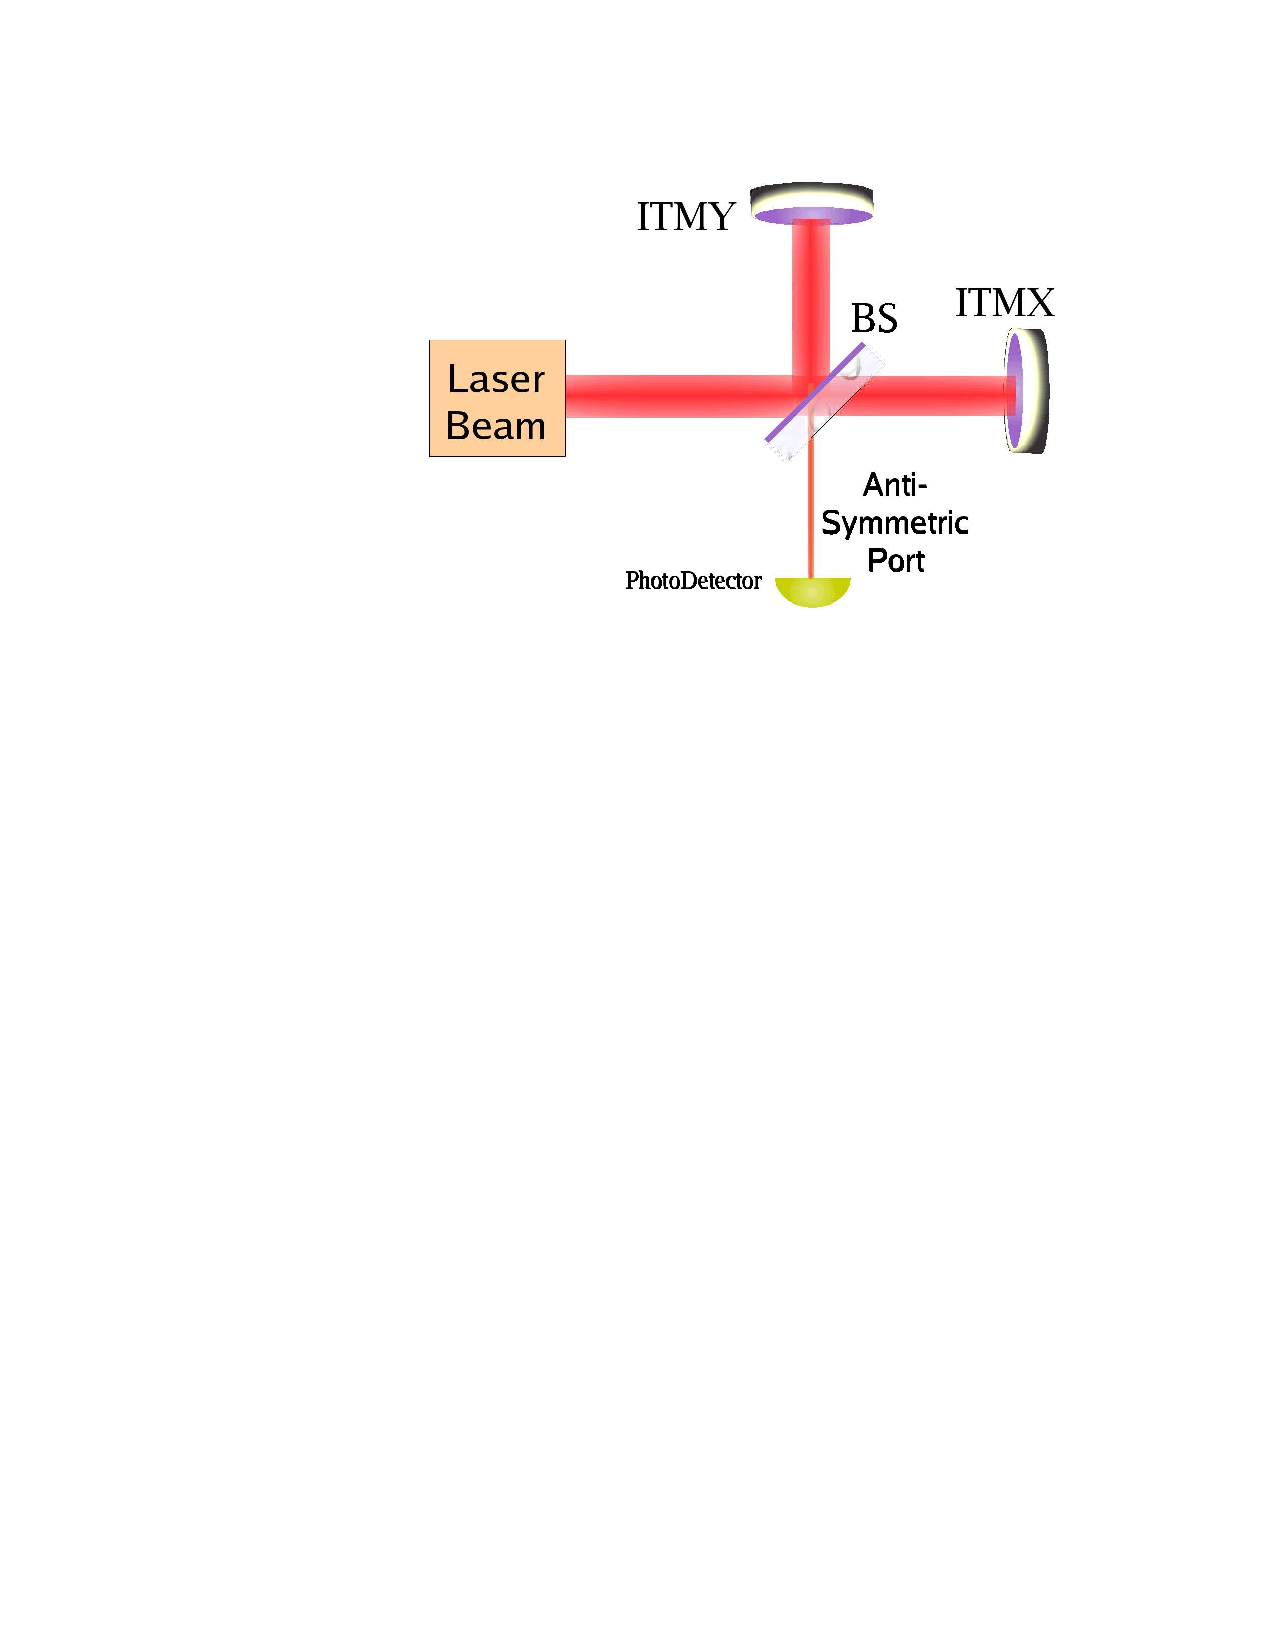
\includegraphics[angle=0,height=3.5in]{Figures/Chap2/Michelson.pdf}}
\caption[Michelson Diagram]{A basic Michelson type interferometer. The field from the
         laser comes in from the symmetric side of the beamsplitter. The light from the
         two arms interferes destructively at the AS port.}
\label{fig:Michelson}
\end{figure}
The resulting electric field at the Anti-Symmetric (AS) port is a function of
the effective optical path difference for the beams in the two arms. 

\begin{equation}
E_{AS} = E_{in} (r_{ex} t_{bs} r_{bs} e^{i 2 \phi_x} - r_{ey} t_{bs} r_{bs} e^{i 2 \phi_y})
\label{eq:SM}
\end{equation}
where  $\phi_x$ \& $\phi_y$ are the phases accumulated by the light in a single trip
down each arm (i.e. $\phi_{rt} = 2 \phi_x$) and $t_{bs}$ \& $r_{bs}$ are the field 
transmission and reflection, respectively,of the beamsplitter.

For an optical interferometer, the electromagnetic radiation is at frequencies
greater than 10$^5$ GHz. This is too high a frequency to detect with present day
technologies. Instead, detectors are used which are sensitive to the envelope of
the field. For visible and near infrared wavelengths, one such detector is the 
photodiode, which emits a current. This photo-electron current is proportional 
to the average photon flux, or power, on the detector.

If we ask what the power at the AS port is for the case in which the end mirrors
have identical reflectivities ($r_{ex} = r_{ey} = r_e$), we get from 
Equation~\ref{eq:SM} that:

$P_{AS} = E^{*}E = 4 |E_{in}|^2(r_e t_{bs} r_{bs})^2 \sin{(\phi_{-})}^2$
where $\phi_{-} = \phi_y - \phi_x$. 
The phase sensitivity is $\frac{d \, P}{d \, \phi_{-}}$. In the simple case where
$r_e = 1$ and $r_{bs} \times t_{bs} = 1/2$, we get

\begin{equation}
\frac{d \, P}{d \, \phi_{-}} = 2 P_{bs} sin(\phi_-) cos(\phi_-) 
\end{equation}
where $P_{bs} \equiv |E_{in}|^2$. The measured power fluctuations due to 
shot noise (more in Section~\ref{sec:ShotNoise}) are:

\begin{equation}
\delta P_{shot} = \sqrt{\frac{2 h c}{\lambda} P_{bs} \sin{\phi_-}^2}
\end{equation}
and so the equivalent \emph{phase noise} is just the ratio:

\begin{equation}
 \begin{aligned}
  \frac{\delta \phi_-}{\sqrt{\mbox{Hz}}} 
         &= \sqrt{\frac{1}{2} \frac{h c}{\lambda} 
            \frac{1}{P_{bs}} \frac{1}{\cos{\phi_-}^2}} \\
         &\simeq 3 \times 10^{-11} \left(\frac{100 \mbox{W}}{P_{bs}}\right)^{1/2}
            \frac{\mbox{radians}}{\sqrt{\mbox{Hz}}}
 \end{aligned}
\label{eq:PhaseNoise}
\end{equation}
where the estimate is for the LIGO laser wavelength of 1064 nm and the phase
offset in the Michelson is small.


\subsection{Fabry-Perot Resonators}

Looking at Equation~\ref{eq:h}, a clear way to increase the strain sensitivity is 
to make very long arms in a
Michelson interferometer. For terrestrial interferometers, the arm length
is limited by technical annoyances such as cost and the availability of a large,
quiet piece of land. A technique which is almost as good as having long
arms is to bounce the beam multiple times in each arm.

This type of delay line~\cite{Herriot}, was proposed \cite{Rai:QPR} as a way 
of increasing the signal gain of the interferometers. Experiments with
this topology \cite{David:Garching} uncovered technical problems due to
scattered light which make this idea impractical, although it has been
pointed out that operating the interferometer with white light is a possibility.

An alternative to this method is to overlap the multiple reflections on 
the same spot on the mirror \cite{Drever:Houches}. By making the
input mirror of the arm into a partial transmitter and adjusting the separation
between the mirrors carefully, the input mirror and end mirror can be made into a
Fabry-Perot resonator \cite{FabryPerot}. The disadvantage with this technique
compared to the delay lines is that the cavity must be operated near resonance
to achieve the high power buildup and resultant phase shift gain which the
delay line has at any operating point. This resonant operation is achieved through
the use of feedback control of the cavity length.




\subsection{Power Recycling}

In the Michelson shown in Figure~\ref{fig:Michelson}, the light returning from
the two arms interferes constructively in the direction heading back to the laser.
Effectively then, the Michelson interferometer looks like a highly reflecting
mirror, when it is adjusted for maximum darkness at the anti-symmetric port.
This reflected light would be dumped somewhere and not contribute to the signal
gain of the interferometer. 

\begin{figure}[!h]
\centerline{\includegraphics[angle=0,height=3.5in]{Figures/Chap2/PRM.pdf}}
\caption[PRM Diagram]{A partially transmitting mirror on the symmetric side
         of a Michelson makes power-recycled Michelson.}
\label{fig:PRM}
\end{figure}
By placing a partially transmitting mirror between the laser and the beamsplitter,
as shown in Figure~\ref{fig:PRM}, one can send this light back into 
the interferometer. The Michelson part of the
interferometer acts on the incoming light like a high reflectance mirror and
can potentially form a high finesse, Fabry-Perot cavity with this new mirror.
This technique is called power 
recycling~\cite{Peter:Thesis,Schilling:Recycling,Drever:Houches} 
and the added mirror is the power recycling mirror (RM).

The following are some further qualitative comments about power recycling which
are more quantitatively described in the following chapters:

\begin{itemize}

\item The RM transmission is chosen to equal as closely as possible, all of the
      other losses experienced by the carrier field in the interferometer (see
      Appendix~\ref{app:optics} for details on losses). 
      The matching is done so that all of the carrier light is coupled into
      the interferometer. The power gain achieved through power recycling is
      $\sim$40-50 in LIGO.

\item The increased power available in the Michelson increases the shot noise 
      limited \emph{phase} sensitivity of the Michelson 
      by putting more light on the Beamsplitter (see Equation~\ref{eq:PhaseNoise}. 

\item The resonance linewidth of the big coupled cavity, formed by the power recycling
      mirror and the arm cavities, is much narrower than the linewidth of the
      arm cavity alone. The coupled cavity pole, $f_{cc}$, is equal to
      $f_c / \mathcal{F}_{RC}$, the arm cavity pole frequency divided by the 
      Finesse of the recycling cavity.
      The beauty of this narrowing is that the \emph{carrier} field which is in the 
      interferometer has been passively filtered by a $\sim$1 Hz low pass filter on 
      top of all of the active stabilization. In this way, we would be able to
      achieve another factor of 100 suppression of the technical laser noise.

\item Power recycling does not reduce the bandwidth of the gravitational wave readout
      at the anti-symmetric port, since differential signals produced in the
      arms \emph{are not recycled}.

\end{itemize}







%----------------- CHAPTER 3 -------------------------------------------
%------ Length Sensing and Control -----------------------------------
%% 
%% Describes the signal extraction for the length DOFs
%% 
%% also the coupling of noise sources on the light
%% 
\chapter{Signal Extraction}
\label{chap:signals}

\begin{figure}[!h]
\centerline{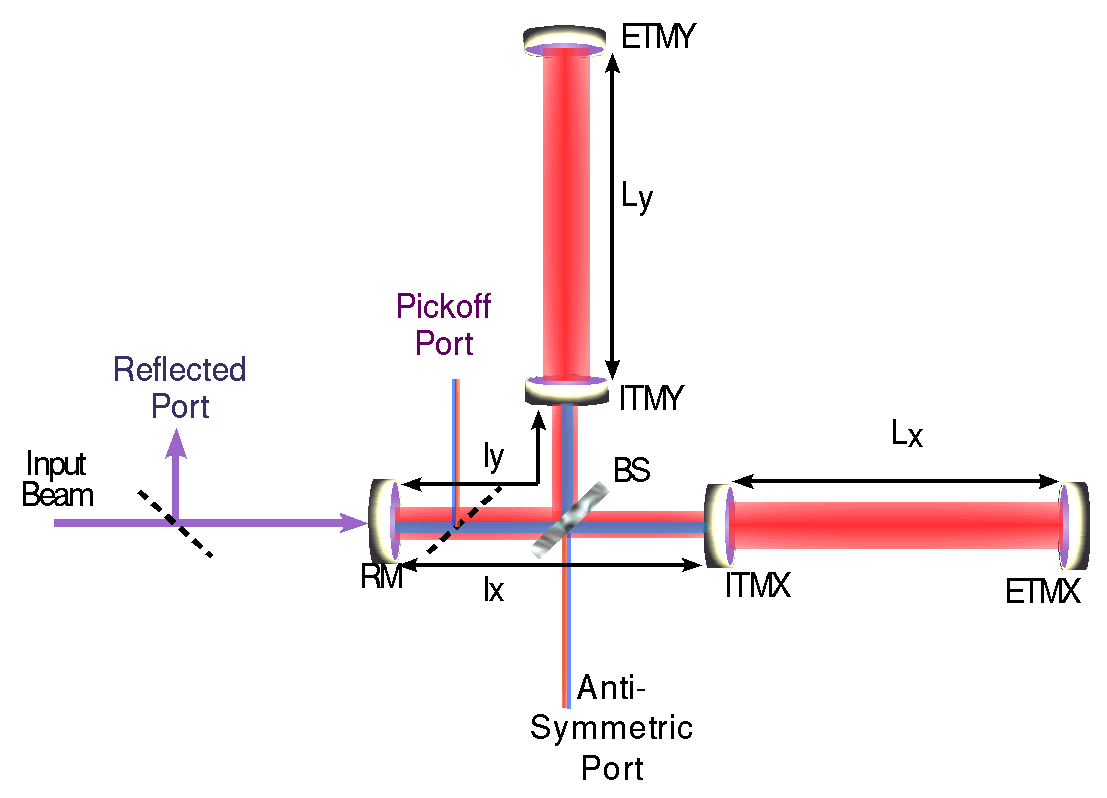
\includegraphics[angle=0,width=6.5in]{Figures/Chap3/IFO2.png}}
\end{figure}
\clearpage

In order to achieve the strain sensitivity goal, multiple resonant cavities
are used to store the light in the interferometer. To keep the cavities
on resonance an active feedback system is employed. This chapter will 
describe how the cavity lengths are sensed and controlled.

\begin{figure}[!h]
\centerline{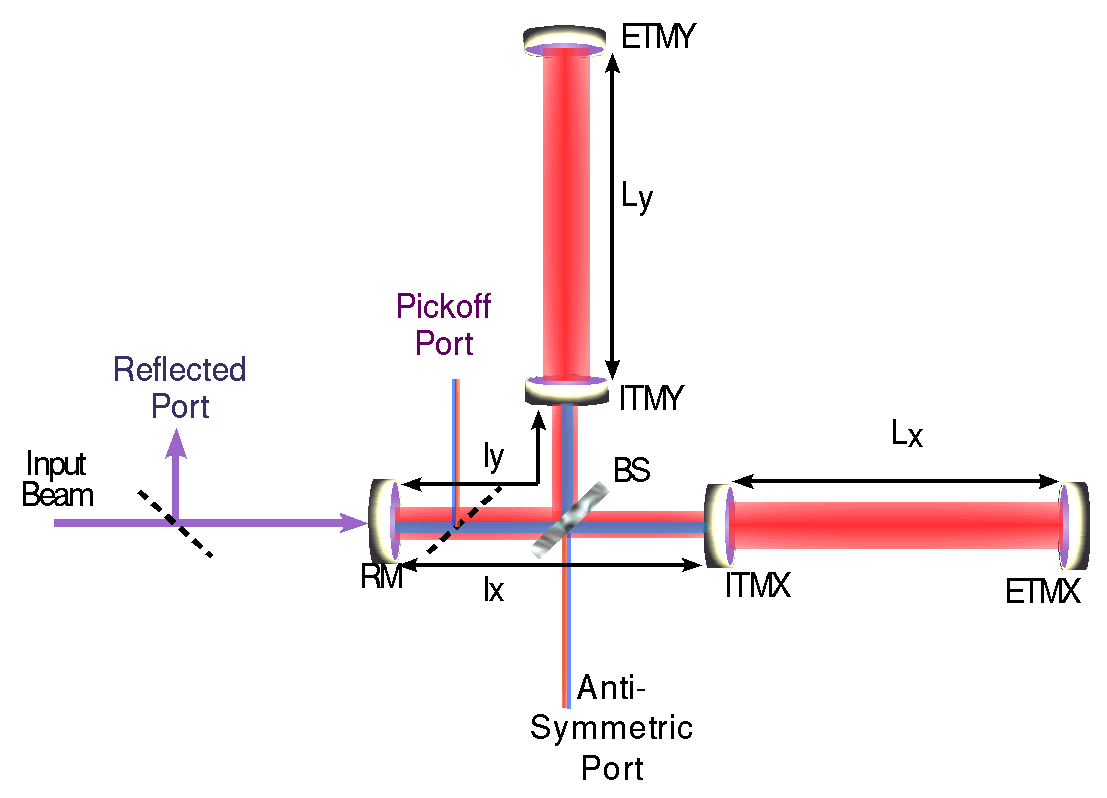
\includegraphics[angle=0,width=6.5in]{Figures/Chap3/IFO2.png}}
\caption[Length Definitions]{Designations of length degrees-of-freedom and signal
                  readout ports. Further details in Appendix~\ref{app:variables}}
\label{fig:DOFs}
\end{figure}



%- - - - - - - - - -  -  -  - - - - - - -  -  -  -   -   -    -    -     -      -
%- - -  SIGNAL READOUT - - - - - - -  -  -  -   -   -    -    -     -      -
%- - - - - - - - - -  -  -  - - - - - - -  -  -  -   -   -    -    -     -      -
\section{Signal Readout Scheme}

The steady state signal readout problem is this: to find the functions that
relate the change of a length with optical signals at the readout ports. 
This solutions is a sensing matrix of the form

\begin{equation}
\vec{V} = \overleftrightarrow{S} \otimes \vec{X}
\end{equation}
where $\vec{V}$ is the vector of voltage readouts, $\vec{X}$ is the vector of
mirror motions, and $\overleftrightarrow{S}$ is the sensing matrix. Each 
element of $\overleftrightarrow{S}$ can be frequency dependent. 

Previous works \cite{Regehr:Thesis,Sigg:FreqResp} have calculated 
this matrix. This section and the rest of the thesis will use the more modern 
notation of \cite{Sigg:FreqResp}. \textbf{Appendix~\ref{app:variables} includes 
the definitions of variables used in the following formulas}.

The physical detector used in the sensing scheme is a photodiode. Since this
detector is only sensitive to power and not the electric field directly, the
trick in the readout is to produce power fluctuations on the readout ports.

To make the measurements at a frequency at which the technical laser noise is
small, the beam incident on the interferometer is phase modulated at 
an angular (radio) frequency, $\omega_m \approx 2 \pi \times$25 MHz. The resulting 
electric field is:

\begin{equation} 
  \begin{aligned} \label{eq:InputBeam}
  E_{in} &= E_0 e^{i \Gamma cos(\omega_m t)} \\
         &\simeq E_0 \left \{ J_0(\Gamma) 
                    + i J_1(\Gamma)e^{+i \, \omega_m t}
                    + i J_1(\Gamma)e^{-i \, \omega_m t}
                    - J_2(\Gamma) e^{+i \, 2 \omega_m t}
                    - J_2(\Gamma) e^{-i \, 2 \omega_m t}
                     \right \}
  \end{aligned}  
\end{equation}
where $\Gamma$ is the modulation depth in radians, $\omega_m$ is the 
modulation angular frequency, $J_n$ is the n$^{\mbox{\tiny th}}$ order Bessel
function of the first kind, and $E_0$ is the unmodulated field of the laser. In
the LIGO interferometers, $\Gamma \approx 0.4$.

The first order Radio Frequency (RF) sidebands and carrier field can be treated
as three fields, each at different frequencies. Each field will have different
reflection and transmission coefficients at each point within the complex coupled 
cavity system of the interferometer. The signal 
readout scheme used in LIGO takes advantage of this dispersion. The scheme is a 
variant of a (now standard) RF reflection locking
technique~\cite{Pound:Locking,Drever:PDH}. To implement this, the 
RF photodetector signal at each port is demodulated at the modulation frequency
used to drive the Pockels cell. The In-phase (cosine) and Quadrature-phase
(sine) components are then separately recorded and/or used in the feedback
control (see Chapter~\ref{chap:controls}).

The naming convention for the interferometer lengths is described in
Appendix~\ref{app:variables}. For the output signals the convention is:
(Port)\_Quadrature. So for example the POB\_Q signal is the quadrature
phase of the demodulated signal from the recycling cavity Pick-Off of the
Beamsplitter. The REFL
signals refer to the signals taken from the light reflected back to the
symmetric port from the interferometer and the AS signals are from the 
Anti-Symmetric port.

As is the convention in \cite{Regehr:Thesis} and \cite{Sigg:FreqResp}, all of
these signal formulae are only valid for frequencies below the arm cavity
free spectral range ($\sim$37.5 kHz for a 4 km cavity). The expressions were
derived using the 'audio sideband' approach: a mirror moving at a frequency,
$f_a$, impresses phase modulation sidebands on the reflected field 
at +/- $f_a$ relative to the incident field. So an incident field with three
frequency components will be reflected with nine frequencies.

Effects from higher order spatial modes are not included here.


%- - - - - - - - - -  -  -  - - - - - - -  -  -  -   -   -    -    -     -      -
%- - - MATRIX ELEMENTS - - - - - - -  -  -  -   -   -    -    -     -      -
%- - - - - - - - - -  -  -  - - - - - - -  -  -  -   -   -    -    -     -      -
\section{Elements of the Sensing Matrix}

\begin{figure}[!h]
\centerline{
\includegraphics[angle=0,width=6.0in]{Figures/Chap3/plant.pdf}}
\caption[LLO Optical Plant]{Plotted are the signal strengths for the L1 interferometer
                in Watts at the modulation frequency per micron of optic
                motion. The solid lines are the diagonal plant elements
                used for the interferometers main length loops. The dashed
                lines are off-diagonal elements. A pickoff fraction of
                80 ppm has been used to calculate the POB signals. All curves are
                for the $\sim$1.6 W of input power in L1 during the S2 run.}
\label{fig:Plant}
\end{figure}
The control system (Chapter~\ref{chap:controls}) adjusts the arm lengths to 
produce a dark fringe
for the carrier. Since the Michelson arm lengths are not equal, dark for the
carrier field does not necessarily mean dark for the sidebands. This arm
length asymmetry ($l_- \approx$ 17 cm) has been designed to transmit a few percent 
of the sideband power from the recycling cavity to the AS port.

Signals at the AS port come from the carrier field beating against the 
static sideband field. Differential changes in the arm cavity lengths ($L_{-}$) 
or in the Michelson length ($l_{-}$) cause a first order differential
phase shift in the carrier fields returning to the beamsplitter from each arm.

\begin{equation}
[ L_{-} \rightsquigarrow AS\_Q ] = -\aleph \, g_{cr} t_{sb} r_{c}'
                          \frac{1}{1 + i f / f_c}
                          k \, \delta L_{-}
\label{eq:darm2asq}
\end{equation}
The notation of the L.H.S. of Equation~\ref{eq:darm2asq}, and all of the following
equations representing elements of the sensing matrix, denotes a transfer
function from one degree of freedom to one readout signal.

Changes occurring faster than the storage time of
the arm cavities do not experience the full buildup of the cavity and are
attenuated compared to low frequencies. Gravitational wave strain signals are read 
out through this same mechanism and so are similarly attenuated at high frequencies.


\begin{equation}
[ l_{-} \rightsquigarrow  AS\_Q ] = \aleph \, g_{cr} t_{sb} r_{c} 
                          \frac{1}{1 + i f / f_c}
                          k \, \delta l_{-}
\label{eq:mich2asq}
\end{equation}
Changes in the Michelson length also show up in this signal but down by a factor of
$r_{c}'/r_{c}$ (which is $\sim 140$ for the LIGO interferometers). This factor is
the 'phase gain' or build-up factor of the arm cavities. Fluctuations above the
arm cavity pole are not resonant in the arm cavities. Since the arms are over-coupled
cavities, the sign of the reflected field changes depending on whether the
incident field is resonant or not. So the high frequencies get a sign flip and
fall out of resonance in the recycling cavity.


The field reflected from the interferometer contains signals contributed by 
both the sidebands and the carrier since both are resonant in parts of the interferometer.

\begin{equation}
[ L_{+} \rightsquigarrow  REFL\_I ] = 2 \aleph \, g_{cr}^{2} r_{sb} r_{c}'
                            \frac{1}{1 + i f / f_{cc}}
                            k \, \delta L_{+}
\label{eq:carm2refli}
\end{equation}
Common mode changes of the arm lengths affect only the carrier field since the sidebands
are not resonant in the arms. This signal has 2 factors of $g_{cr}$ in it; one, 
since the carrier field in the arms is amplified by the recycling cavity and 
another, because the common arm signal is resonant in the recycling cavity. 
At the reflected port, these carrier audio sidebands beat against the static 
RF sidebands.


\begin{equation}
[ l_{+} \rightsquigarrow  REFL\_I ] = 2 \, \aleph \, \left [ g_{sb}^{2} r_{cr} r_{M}  
                            + g_{cr}^{2} r_{sb} r_{c} 
                            \frac{1}{1 + i f / f_{cc}} \right ]
                            k \, \delta l_{+}
\label{eq:prc2refli}
\end{equation}
The REFL\_I signal produced by a change of the power recycling cavity average length 
($l_{+}$) is more complicated. Since both the sidebands and carrier are resonant in 
the recycling cavity, both are modulated by the $l_+$ length change. The carrier 
component is filtered above $\sim$1 Hz by the coupled cavity resonance and so the main 
contribution above 100 Hz is from the RF sidebands' audio sidebands beating 
with the static carrier.


\begin{equation}
[l_{-} \rightsquigarrow  REFL\_Q ] = - \aleph \, g_{sb} t_{sb} r_{cr} k \, \delta l_{-}
\label{eq:mich2reflq}
\end{equation}
The quadrature phase signals at the REFL and PO ports are produced in a
different way. Changes in the Michelson length change produce differential changes
in the sideband fields reflected from the Michelson back towards the RM. At the
reflected port, the difference between the amplitudes of the upper and lower
sidebands produce a signal 90 degrees out of phase with the REFL\_I signal. In
a symmetric arm length Michelson interferometer, there would be no Q-phase
signal, since the reflectivity for the sidebands would be a quadratic
function of $l_{-}$.



\begin{equation}
[ L_{+} \rightsquigarrow  POB\_I ] = -2 \aleph \, \frac{g_{cr}^{2} g_{sb}}{t_{RM}} r_{M} r_{c}'  
                  \frac{1}{1 + i f / f_{cc}} k \, \delta L_{+}
\label{eq:carm2pobi}
\end{equation}
The signal from the pick off inside the recycling cavity is very similar to the
one in reflection. The main difference being that it does not depend delicately
on the coupling of the sideband to the recycling cavity, but instead is produced
by beating the carrier audio sidebands against the resonant sideband field.


\begin{equation}
[ l_{+} \rightsquigarrow  POB\_I ] = 2 \aleph \, \frac{g_{cr} g_{sb}}{t_{RM}} r_{M} r_{c}  
                  \left[g_{cr} \frac{1}{1+i\frac{f}{f_{cc}}} -g_{sb}\right]
                  k \, \delta l_{+}
\label{eq:prc2pobi}
\end{equation}
Very similar to the $[l_{+} \rightsquigarrow REFL\_I]$ element. The main difference
is that the local oscillator field is the carrier field inside the recycling cavity
instead of the carrier reflected from the interferometer.

\begin{equation}
[ l_{-} \rightsquigarrow  POB\_Q ] = -\aleph \, \frac{g_{cr} g_{sb}^2}{t_{RM}} t_{M} 
                                      k \, \delta l_{-}
\label{eq:mich2pobq}
\end{equation}
This element also appears to be similar to the REFL port element but there are two
important differences. First, the signal is independent of the sign of the
carrier coupling since it uses the internal recycling cavity field. Second, the
dominant carrier field in reflection can be the non-modematched component. This
will produce a spurious signal through beating with non-modematched sideband
field.

Since each readout signal is sensitive to multiple degrees of freedom there is some
choice to be made in selecting a particular configuration.
It is fairly clear from these equations and Figure~\ref{fig:Plant} that only AS\_Q 
may be used for reading out the differential arm length. This leaves some other 
combination of the Q-phase signals to read out $l_{-}$. In the absence of 
beam distortions, we would be free to choose whichever combination of the two
gives the best SNR. In the case of the $l_-$ readout, we use the POB\_Q signal
to avoid the junk signal from the mode-mismatch of the carrier and sidebands.

The case for the common mode signals is a little less clear, since in both REFL\_I 
and POB\_I the $L_{+}$ signal is totally dominating the weak $l_{+}$ signal. In a 
perfectly stable, noiseless interferometer
one could take this 2 $\times$ 2 signal matrix and invert it properly to
obtain linearly independent readouts of both degrees of freedom. 

In the real world, this is problematic for two reasons: first, the small fraction of 
light  from the internal recycling cavity pickoff is
so small ($\sim$100 ppm) that the signal-to-noise ratio is much poorer than
the reflected port where all of the light is available and second, even if
the noise were not an issue, this matrix inversion would require subtracting two 
large signals
to produce a very small signal (the $l_+$ signal) and would be overly sensitive
to variations in the optical gain at the REFL and POB ports. To avoid these
issues, the REFL\_I signal is fed back to the laser frequency with a high gain, 
high bandwidth loop (see Section~\ref{sec:CMservo}), effectively driving the 
REFL\_I signal 
to zero. Solving for the newly flattened plant by setting $\mbox{REFL\_I} = 0$, 
gives a new solution for POB\_I which is only sensitive to $l_{+}$:

\begin{equation}
[ l_{+} \rightsquigarrow  POB\_I ] = - 2 \aleph \, \frac{g_{sb}^2 r_M}{t_{RM}r_{sb}}
                           \left [ g_{cr} r_{sb} r_c + g_{sb} r_{cr} r_M \right ]
                           k \, \delta l_{+}
\end{equation}


%- - - - - - - - - -  -  -  - - - - - - -  -  -  -   -   -    -    -     -      -
%- - - DARK PORT SIGNALS - - - - - - -  -  -  -   -   -    -    -     -      -
%- - - - - - - - - -  -  -  - - - - - - -  -  -  -   -   -    -    -     -      -
\section{Dark Port Signal Generation}
\label{sec:darksignals}

Equation~\ref{eq:darm2asq} only deals with the Q phase signal which we use for
the gravitational wave signal readout and the differential arm length control.
It was assumed that the only carrier field at this port comes from the differential
arm length offset. However, a carrier field may also exist in the other phase.
In principle, this should not produce a signal unless there is a corresponding
sideband field in the ``wrong`` phase. Including fields in both phases we get:

\begin{equation}
 \begin{split}
  \frac{E_{AS}}{E_{0}} =& J_{0}(\Gamma) g_{cr} \left [ \frac{\delta r_c}{2} 
                                         + i r_{c}' k \Delta L_- \right ] \\
 \times & J_{1}(\Gamma) t_{M} \left [ \frac{\delta g_{sb}}{2} \cos{\omega_{m} t}
                           + i 2 g_{sb} \sin{\omega_{m} t} \right ]
 \end{split}
\end{equation}
where we have included two asymmetries: $\delta r_c$ is the difference in the
arm cavities' resonant reflectivities for the carrier and $\delta g_{sb}$ is
the difference in the recycling gain between the upper and lower 
first order RF sidebands.

The AS\_Q signal is produced by the beat between the imaginary part of the
carrier field and the imaginary part of the sideband field. The AS\_I signal
is produced by the real components and only exists in the presence of the
two asymmetries.
\begin{equation}
S_{\mbox{\tiny AS\_I}} = \frac{1}{8} \aleph \, g_{cr} t_{M} 
                         \, \delta r_c \, \delta g_{sb}
\label{eq:ASI}
\end{equation}

%----------------- CHAPTER 4 -------------------------------------------
%--------NOISE-----------------------------------------------
%% Divides the noises into displacement noise and sensing noise.
%% 
%% 
%% 
\chapter{The Noises}
\label{chap:noise}

\begin{figure}[!h]
\centerline{\includegraphics[angle=0,width=6.5in]{Figures/Chap4/S3noise.pdf}}
\end{figure}
\clearpage

There are many noise sources in the LIGO interferometers. In this chapter,
those noises which contaminate the gravitational wave readout channel and are 
of a comparable amplitude to the strain noise goal are described.

The noises are categorized as either a displacement noise, one which directly
moves the suspended mirrors, or as a sensing noise, one which appears in the
readout signal but is not caused by a gravitational wave.



%- - - - - - - - - -  -  -  - - - - - - -  -  -  -   -   -    -    -     -      -
%- - -  DISPLACEMENT NOISES - - - - - - -  -  -  -   -   -    -    -     -      -
%- - - - - - - - - -  -  -  - - - - - - -  -  -  -   -   -    -    -     -      -
\section{Displacement Noises}
The displacement noises in this section are only those that cause a differential
change in the arm cavity lengths. We are also mainly concerned with noise in
the 40-7000 Hz band where the interferometer is designed to be sensitive to
gravity waves.


%-------------------------------------------------------
\subsection{Seismic Noise}
The test mass mirrors are on the earth and so vibrations of the earth's
surface could directly show up as a strain noise. A rough estimate for 
the displacement spectral density of the ground noise above 0.1 Hz at a quiet site is 
$x(f) = \frac{10^{-8}}{f^{2}} \frac{\mbox{m}}{\sqrt{\mbox{Hz}}}$. 
At 100 Hz, this would still be 7 orders of magnitude above the 
LIGO displacement noise goal. A combination of passive and active 
isolation techniques are used to reduce the seismic coupling.

\begin{figure}[!h]
\centerline{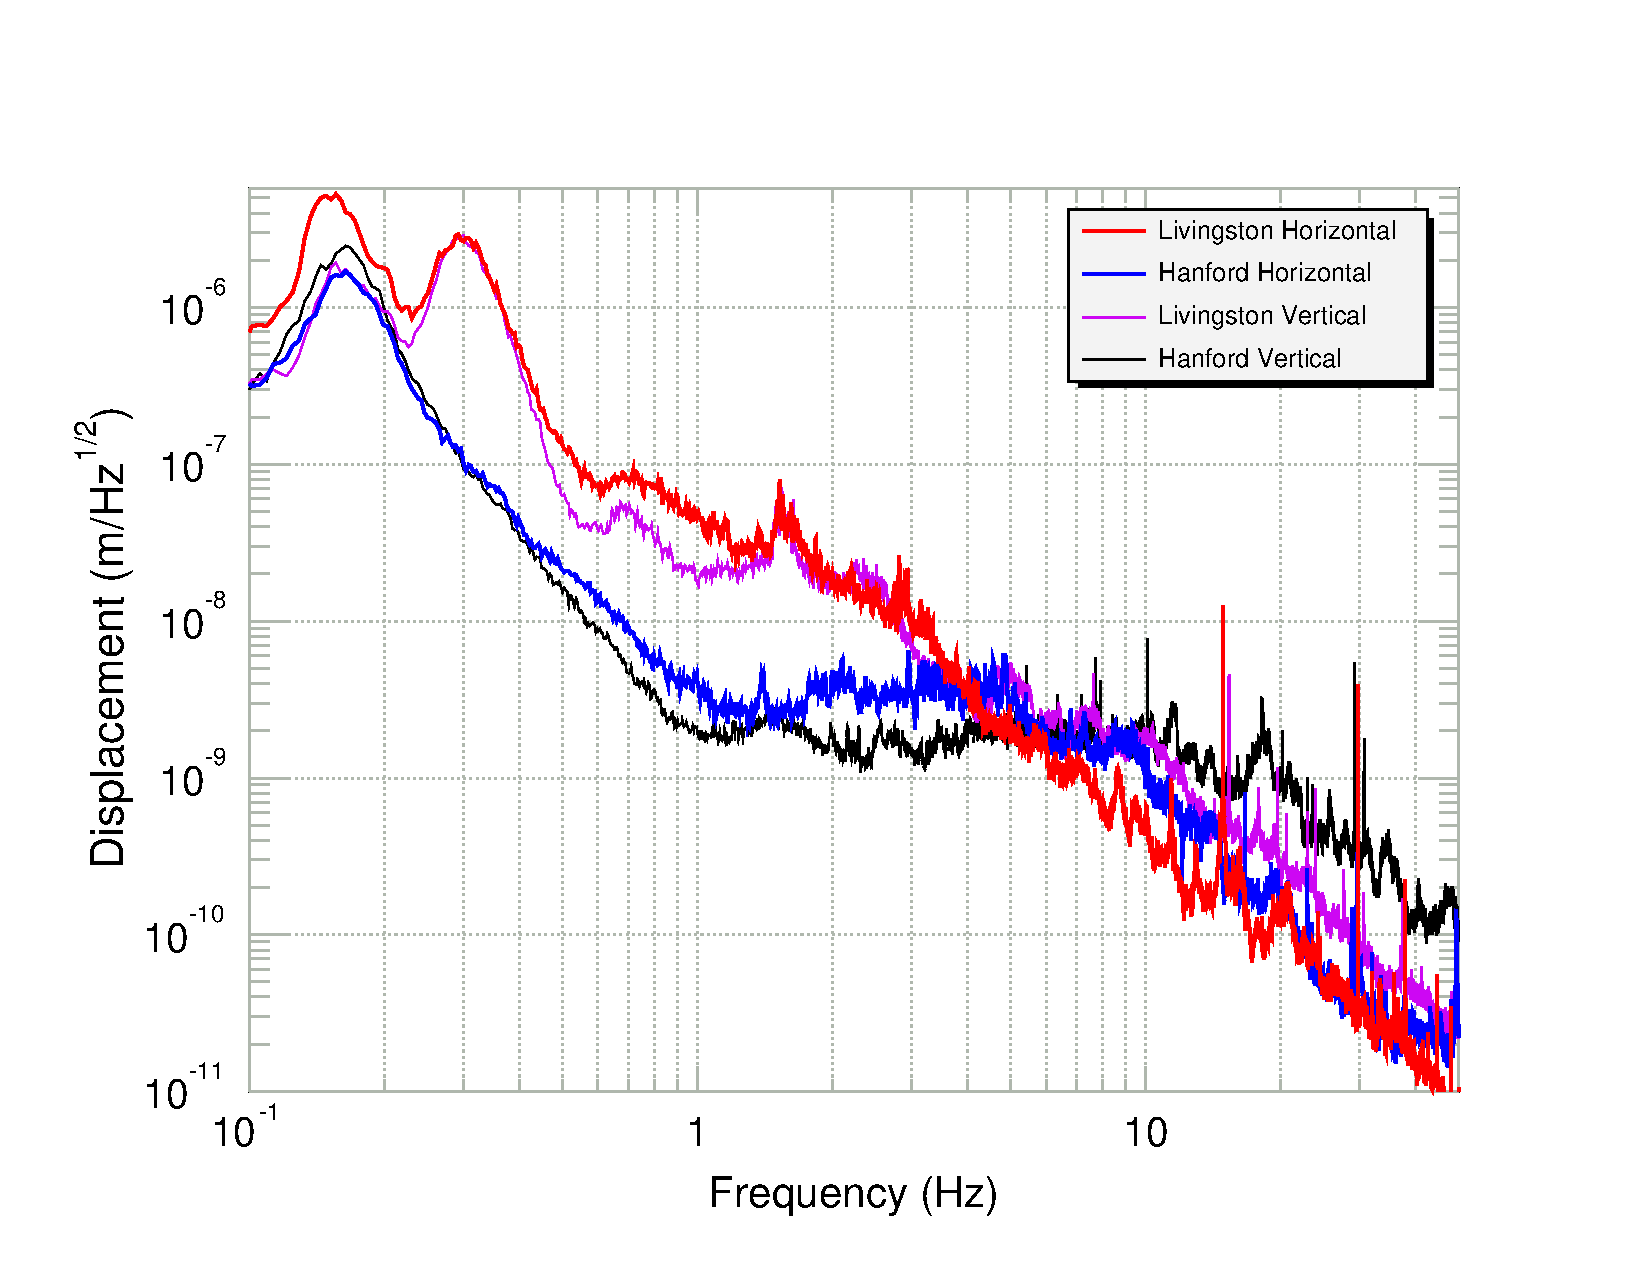
\includegraphics[angle=0,width=6.5in]{Figures/Chap4/LLOLHO-seis2.pdf}}
\caption[Seismic Spectra]{Amplitude spectral density of the daytime displacement 
                          noise of the ground at both LIGO sites.}
\label{fig:SeismicNoise}
\end{figure}

\subsubsection{Noise Characteristics}
\label{sec:SeismicCharacter}

\begin{itemize}
\item Excepting dramatic events such as earthquakes and subway cars, the largest
      ground motions seen everywhere are from the $\approx$6 second period 
      `microseism' \cite{useism}.
      The primary microseism is generated by ocean waves having a $\approx$12-15 second
      period. The secondary microseism, which is much larger, is produced
      by standing waves on land from a large number of sources.

\item The power in the 0.5-10 Hz band is largely due to man made noise. 
      The operation of the Livingston interferometer has been
      seriously impaired by this noise. The noise is so large that the
      interferometer only operates reliably from the end of the workday
      (6-8 PM on weekdays) until the beginning of the workday (5-6 AM).

\item Above 10 Hz, most of the noise is self inflicted. The acoustic and 
      vibrational environment at the observatories has been compromised 
      by the HVAC systems. 
      Efforts are underway to remediate this by balancing fans, installing 
      acoustic isolation and damping material, and isolating the noisiest components 
      with springs.
\end{itemize}


\subsubsection{Seismic Isolation}
To attenuate this noise, the core interferometer optics are each suspended
as pendula (see Section~\cite{sec:SUS}) by a single loop of steel wire. 
The pendulum length is set to put the resonant frequency 
to $f_{p} \simeq 0.75$ Hz. 
This reduces the coupling between ground noise and optic motion by 
$\sim(\frac{f_{p}}{f})^{2}$ above $f_p$.
\begin{figure}[!h]
\centerline{
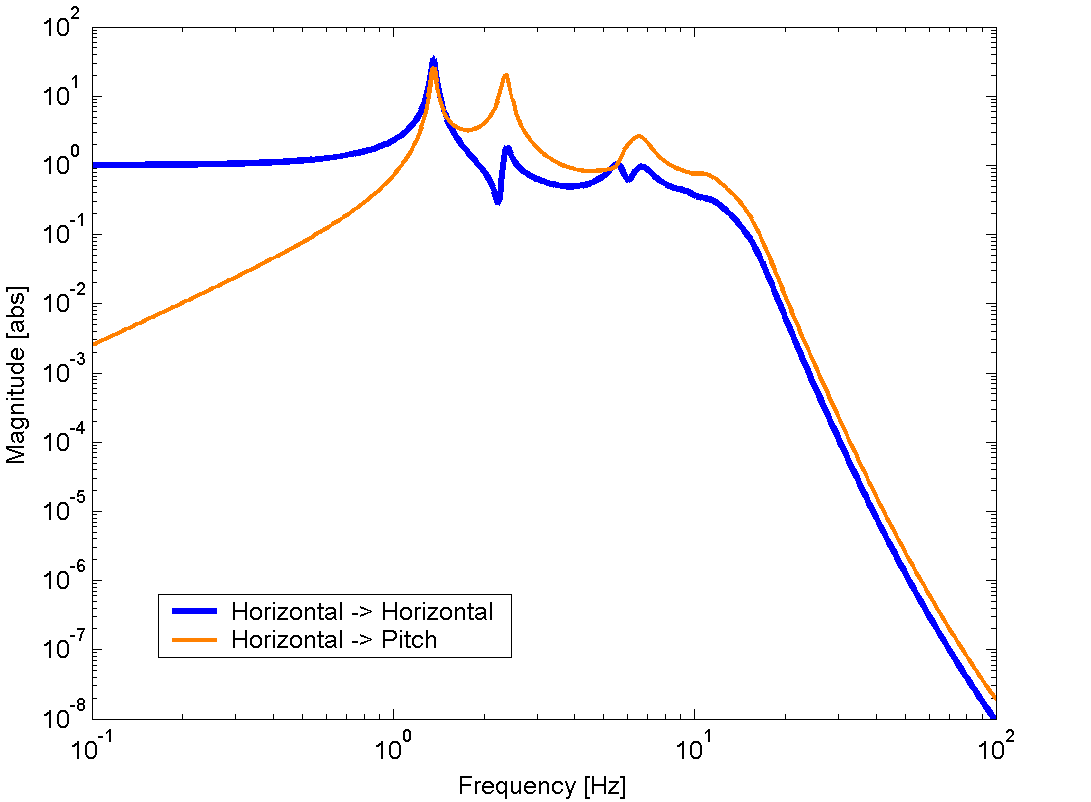
\includegraphics[angle=0,width=6.5in]{Figures/Chap4/BSCtf2.png}}
\caption[BSC Stack Transfer Function]{Modeled Isolation Stack Transfer Functions.}
\label{fig:StackTF}
\end{figure}
To get the rest of the required attenuation, the pendulum structure is placed upon
a stack of four alternating mass-spring layers (see Figure~\ref{fig:BSC}). Each of 
these layers gives another attenuation
factor proportional to $f^{-2}$, giving $\approx$100 dB of attenuation at 40 Hz and 
$>$140 dB at 100 Hz\cite{Giaime:ShitStack}.


%-------------------------------------------------------
\subsection{Thermal Noise}

At frequencies where seismic motion has been sufficiently filtered, the
interferometer's strain sensitivity will be limited by thermal noise.

The suspended mirror is in a radiative thermal equilibrium with the vacuum
chambers which are at room temperature. The thermal motions of the individual
particles of the glass, the mirror coating, and the mirror's suspension system
can cause fluctuations in the measured cavity length.

The reason that the thermal energy of the whole mirror / suspension system 
comes into play is that there is a coupling between all of the internal modes 
of the system and the motion of the mirror's surface. This coupling ensures 
that there is a continuous flow of energy between the degree of freedom we 
are trying to measure and all of the other internal degrees of freedom. 

The energy flow works both ways; the energy in one of the mirrors modes will
slowly dissipate as it couples into all the other modes. A general theme in
the thermal noise reduction game is reducing, as much as possible, all sources
of dissipation which damp motions \emph{in the degree of freedom we are
measuring}.

The relation between the amount of fluctuation of the mirror surface
and the dissipation in the system is described by the 
Fluctuation-Dissipation theorem\cite{Callen:FD}:

\begin{equation}
S_{x}(f) = \frac{k_{B} T}{\pi^{2} f^{2}} Re[Y(f)]
\end{equation}
where $S_{x}(f)$ is the power spectral density of fluctuations in a degree of
freedom $x$, $k_B$ is Boltzmann's constant, $T$ is the temperature of the system,
$f$ is the frequency of the motion and $Y(f)$ is the complex mechanical admittance 
(inverse of the impedance) of the system. One expression for admittance which 
is particularly useful is\cite{Saulson:Book}:

\begin{equation}
Y(f) = \frac{v(f)}{F_{therm}} = i \frac{2 \pi f \, x(f)}{F_{therm}}
\end{equation}
where $F_{therm}$ is the thermal driving force, $x$ is the readout variable,
and $v$ is the time-derivative of the readout variable.

In the case of a Fabry-Perot cavity, we are principally interested in one
degree of freedom: the one that makes a signal in our strain readout
channel. It takes a very special type of test mass motion to make it to
this signal port. Thermal fluctuations excite all of the internal degrees
of freedom of the mirror (pitch, yaw, roll, pringle), but most of these mirror 
surface motions only scatter light out of the cavity's fundamental mode 
into higher order modes which do not resonate in the cavity. The strain noise
that we measure comes from piston motions of the mirror along the cavity axis
(there are some small couplings between the degrees of freedom so in principle
we have to also ensure that the noise in the non-critical degrees of freedom is
not too large).

In the LIGO interferometers, we can separate the thermal noise sources into two
convenient categories: the fused silica mirrors which form the arm 
cavities and the steel suspension wire which supports the optics.

%-------------------------------------------------------
\subsubsection{Test Mass Thermal Noise}

The original estimates of test mass thermal noise made in the 20th century were
based on a normal mode decomposition of the optic's internal modes 
\cite{Fred:Thermal}. However, this method requires one to measure the
Q of every mechanical resonance up to $\sim$100 kHz in order to 
estimate the thermal noise accurately. A more direct approach described
by Gonz\'alez and Saulson\cite{Gaby:Acoustic}, applied to mirrors by 
Levin\cite{Levin:Thermal}, is to calculate the admittance for our 
readout variable, assuming a homogeneous loss in the bulk.

In addition to loss in the glass substrate of the mirror, loss in the dielectric 
coatings on the face of the optic\cite{Andri:Coatings} has been identified
as a significant source of thermal noise. Approximately 30 
alternating, 1/4 wavelength, layers of Ta$_{\mbox 2}$O$_{\mbox 5}$ 
and SiO$_{\mbox 2}$ are used to make the coatings. Although the amount of coating
material is small compared to the size of the mirror, its mechanical losses
are $\sim$1000 times greater than the fused silica substrate. 

The power spectral density of displacement noise for 
a single mass is \cite{Andri:Coatings}:

\begin{equation}
\label{eq:InternalThermal}
S_x(f) \simeq  \frac{2 \, k_B T}{\pi^{3/2} \, w \, Y_S \, f} \left[ \phi_S +
                   \frac{2 \, d_{\mbox{\tiny C}}}{\sqrt{\pi} \, w} \phi_C \right]
\end{equation}
The nominal values for these parameters are listed in Table~\ref{t:LOS}. Using the best
guess estimates at the time of this writing, the thermal noise from the substrate
is approximately the same as that from the coatings. The total substrate thermal noise
contribution from all four mirrors is:
\begin{equation}
\delta L_{-}(f) \simeq 5 \times 10^{-20} 
                  \left(\frac{100 \, \mbox{Hz}}{f}\right)^{1/2}
                  \left(\frac{\phi_S}{1 \times 10^{-7}}\right)^{1/2}
                  \frac{\mbox{m}}{\sqrt{\mbox{Hz}}}
\end{equation} 
The coating thermal noise contribution is:
\begin{equation}
\delta L_{-}(f) \simeq 2.5 \times 10^{-20} 
                  \left(\frac{100 \, \mbox{Hz}}{f}\right)^{1/2}
                  \left(\frac{\phi_C}{2 \times 10^{-4}}\right)^{1/2}
                  \frac{\mbox{m}}{\sqrt{\mbox{Hz}}}
\end{equation}
taking into account that the ETM coatings have almost twice as many layers as the
ITM. There are some indications~\cite{Gregg:Pie} that the intrinsic loss in fused
silica can be as low as 10$^{-8}$. If this turns out to be the case for the LIGO optics
then the total mirror thermal noise contribution to the interferometer strain noise
would be reduced by a factor of $\approx2$.

%-------------------------------------------------------
\subsubsection{Suspension Thermal Noise}
\label{sec:SUSthermal}
The core optics in the interferometer are each suspended by a single loop
of steel music wire, $\approx$0.3 mm in diameter. The thermal noise for the LIGO 
suspensions has been previously analyzed~\cite{Gaby:Thermal} using a full 6 
degree of freedom model of a mirror supported by an anelastic steel beam. 
The often used model for the loss is that of a frequency independent internal
friction. The following section compares the model predictions with the data 
from the interferometers.

As in the above case of test mess thermal noise, there are 2 pieces of
information needed to estimate the noise contribution: The transfer function
between force and test mass motion (the admittance) is one. The other is the
source term: in our case random thermal forces distributed over the suspension
structure.

The admittance is known and can easily be calculated numerically. The thermal
force distribution, however, depends on the loss distribution in the system.

One of the dirt effects in suspension thermal noise is excess loss introduced
at the suspension point \cite{Kovalik:Clamps}. This can 
come from rubbing due to improper clamping of the suspension 
wire~\cite{Kovalik:ClampSpeech}. This excess source of loss is difficult to
determine ahead of time and can best be established by in-situ measurements.
This was done by measuring the quality factors of the 'violin' modes of the
suspension wire in two ways:

First (the easiest way, after the fact) the power spectrum of the strain
channel was examined. Vibrations of the 
mass from the thermal fluctuations in the wire dominate the signal in the
340-360 Hz band. Due to slight asymmetries in the suspensions (such as wire
thickness, length and cross-sectional ellipticity), each side of
the wire loop has a slightly different frequency.

\begin{figure}[!h]
\centerline{
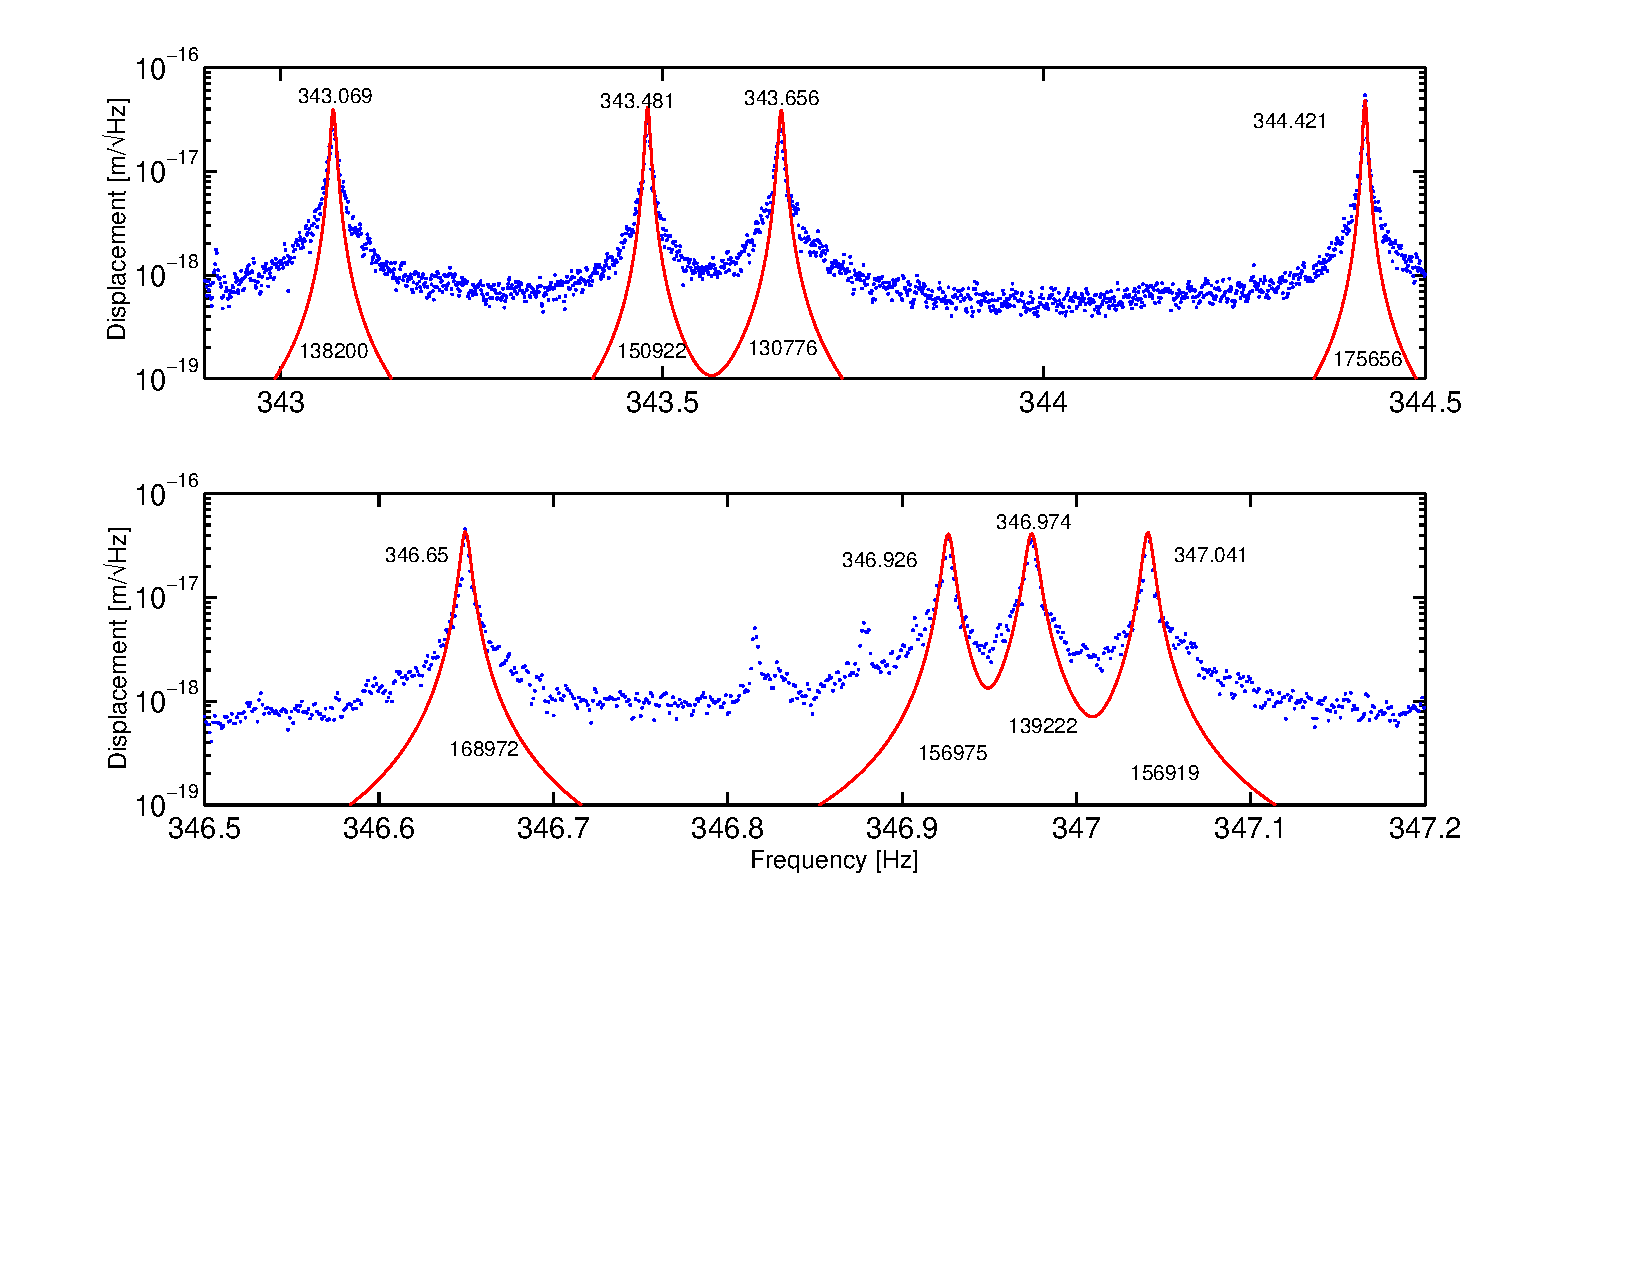
\includegraphics[angle=0,width=6.5in]{Figures/Chap4/violins.pdf}}
\caption[Violin Modes]{Displacement noise from the suspensions' violin
         modes. Plotted also is the fit to the data and the fitted
         frequencies and Q's.}
\label{fig:ViolinModes}
\end{figure}
A non-linear least squares fit to a Lorentzian curve was performed on each
peak. The frequency and Q from each fit is shown in Figure~\ref{fig:ViolinModes}.
Using the model from \cite{Gaby:Thermal}, we can place an upper limit on the average
loss angle for the violin modes of $\phi \lesssim 0.001$. From the fit we can see
that there is excess power in the wings of each peak; there is more than one
expects from a simple Lorenzian model for the peak. One possible source of this
excess noise is drift in the interferometer's optical gain on several minute
time scales. The next iteration of this measurement will have to use a gain corrected
displacement readout.


% Loss angle in steel:
% --------------------
% Virgo - C85 steel  1e-4
%
% Gaby - Paper       1e-3


Another weakness of this method is that it relies on several hours of
data in which the interferometer is assumed to be static. In reality,
a 1 degree C change in the temperature of the wire would result in a 10X
larger drift ($\approx$30 mHz) than what we are trying to measure.

To avoid the drift issues one would like to make a quick measurement.
One way is to measure the decay time for violin mode excitations
which only takes $\tau = Q/(\pi f_{vio}) \simeq 100$ seconds. This has the
drawback of interrupting science data taking but in principle has a much better
chance of success and should be pursued in the future to better estimate
the suspension thermal noise.


%-------------------------------------------------------
\subsection{Radiation Pressure}
\label{sec:radpress}

Technical radiation pressure noise comes from power fluctuations
of the input beam coupling to differential displacement noise through slight
asymmetries in the arms. Characterization of the LIGO optics (see \cite{COCwebsite}
and Appendix~\ref{app:optics}) allows us to estimate these couplings. 
Three sources of asymmetry are:

\begin{itemize}
\item Imbalance in the masses of the mirrors. ($\sim 0.3 \%$)
\item Imbalance in the arm cavity buildups. ($\sim 2 \%$)
\item The beamsplitter splitting ratio is not exactly 50/50. ($\sim 0.5 \%$)
\end{itemize}
For this noise to pose a problem, the power fluctuations on the input beam
must be rather high. Since the double cavity resonance attenuates all carrier
power fluctuations above 1 Hz, we find that in our signal band the contribution
is a few orders of magnitude below the sensitivity goal.


\subsubsection{Quantum Radiation Pressure}
Quantum radiation pressure, however, is not attenuated in this way. Quantum
mechanical radiation pressure noise in the interferometer comes from the
zero point fluctuations of the vacuum field which enters through the dark
port of the Michelson~\cite{Caves:RadPress}. A field which enters through the
dark port affects the two arms differentially. These fluctuations give rise to
a fluctuating force. The resulting displacement is:

\begin{equation}
x(f) = 2 \times \frac{2 \, \delta P}{m c (2 \pi f)^2}
                = \frac{1}{2 \pi^2 m c f^2} \sqrt{\frac{2 h c P}{\lambda}}
\end{equation}
The differential displacement for a nominal set of parameters is:

\begin{equation}
\Delta L_{-}(f) \thickapprox 10^{-22} \left(\frac{10.5 \mbox{kg}}{m}\right) 
                                      \left(\frac{100 \mbox{Hz}}{f}\right)^2
                           \left(\frac{P_{in}}{1 \mbox{W}}\right)^{1/2}
                            \frac{\mbox{m}}{\sqrt{\mbox{Hz}}}
\end{equation}
which is far below any reasonable estimate for the interferometer noise floor.


%-------------------------------------------------------
\subsection{Actuator Electronics Noise}

Usually when interferometer noise is described, things like
seismic, thermal, and shot noise are considered. As of this writing, the
noise source which has gotten the most work has been electronics noise in
the test mass actuator.

\begin{figure}[!h]
\centerline{
\includegraphics[angle=0,width=6.5in]{Figures/Chap4/actuation.jpg}}
\caption[Actuation Electronics]{The chain of digital and analog filters
         beginning with the pre-DAC whitening and ending with the box
         driving the current into the actuator coils}
\label{fig:OutputElectronics}
\end{figure}

The electronics which drive the test masses span the largest dynamic
range of any piece of electronics in the system. At the low frequencies it must correct
for the large ground fluctuations caused by storms and humans, whereas at
$\sim$100 Hz it must be quiet enough to not mask the gravitational wave
signals.

\subsubsection{Coil Driver}
\label{sec:CoilDriver}
The final electronics unit which drives the coils for the suspended optic
(described in Section~\ref{sec:OSEMdesc}) is called the coil driver.
There are 2 competing requirements on the coil drivers. They must have
a low enough spectral density of current fluctuations that this electronics
noise fall below other more fundamental noises (seismic, thermal). They
must also be able to provide enough force to acquire lock and maintain the
cavity resonance in the presence of large seismic disturbances.

The following figure shows how the low noise ({RUN} mode) and large range
{(ACQUIRE} mode) are accommodated.

\begin{figure}[!h]
\centerline{
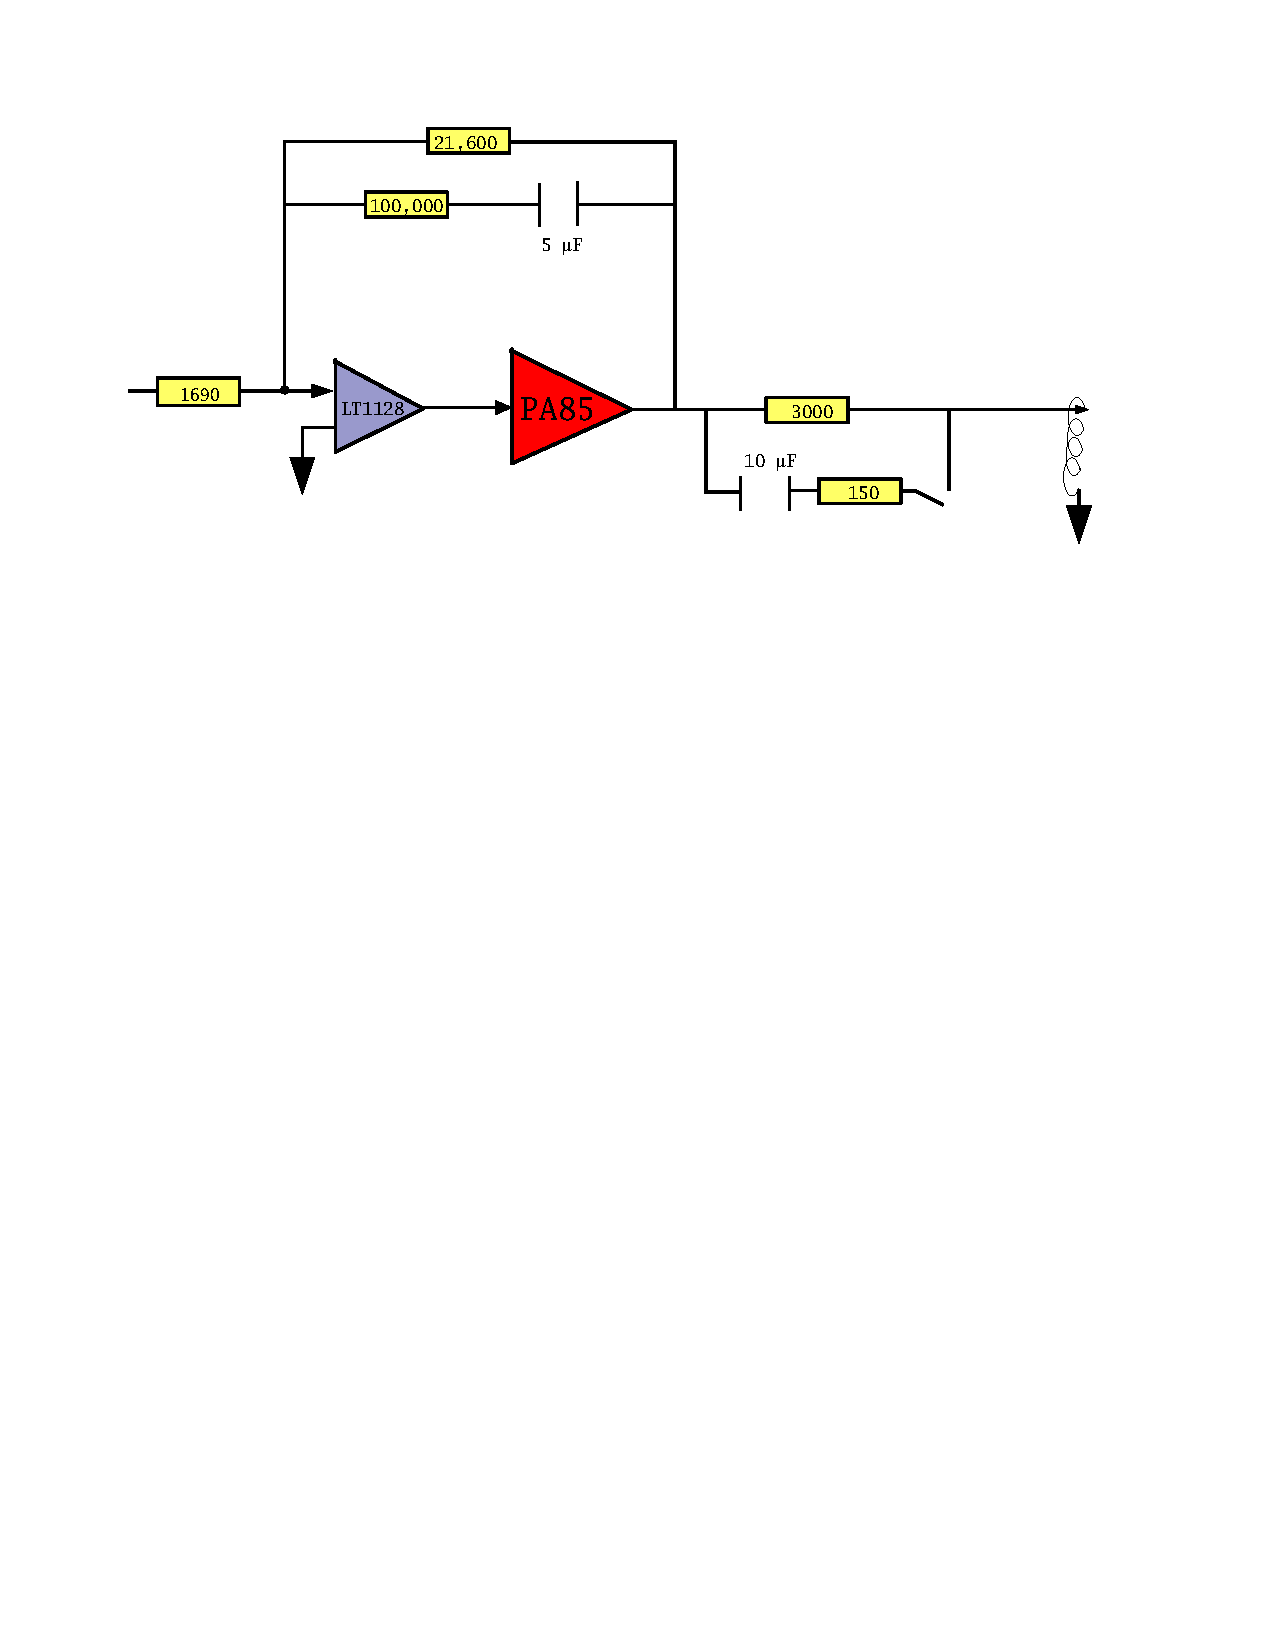
\includegraphics[angle=0,width=6.5in]{Figures/Chap4/coildriver.pdf}}
\caption[Coil Driver]{Simplified block diagram of the coil driver
         circuit for one face coil on one of the large optics. Closing
         the relay transitions from {RUN} to {ACQUIRE} mode. The yellow
         rectangles are resistors and the two spaced lines are capacitors.}
\end{figure}
A high voltage power amplifier (+/- 150 V, PA85) supplies current to the actuator coil
through a series resistor. In order to have a large dynamic range for lock
acquisition, a remotely controlled relay can engage a low impedance bypass
around the large series resistor. This gives a factor of $\sim$20 more force.

Since the servo system must hold the cavity within its narrow linewidth
during the switch a digital filter is employed to compensate the different
analog transfer functions. After acquiring lock the relay is switched
open and the digital compensation filter is turned off, leaving the
overall transfer function unchanged.

%The switching transient from this was large enough to move the 
%optic by $\sim$5 nm, breaking the lock. So a delay was


%-------------------------------------------------------
\subsubsection{DAC Noise}

Since the servo which controls the differential arm length is digital, the
drive signal to the coil driver must pass through a digital-to-analog
converter (DAC).

%The theoretical dynamic range for a DAC is:
%\begin{equation}
%V_{noise}(f)/\sqrt{Hz} = \frac{V_{p-p}/N_{bits}}{\sqrt{12 F_{s}}}
%\end{equation}

The LIGO DACs are 16-bit and have a 16384 Hz sampling rate. The dynamic
range (V$_{pp}$/V$_{noise}$(f)) is $\approx10^6$ in a 1 Hz bandwidth.

By contrast, the coil current spectrum must be able to supply 10 mA$_{\mbox{pk}}$ at
very low frequencies to accommodate the microseism and have a noise of less
than $10 \mbox{pA}/\sqrt{\mbox{Hz}}$ from 40-150 Hz. This gives a $\sim$1000X mismatch
in the dynamic range between the DAC and the optic's coil currents.

To satisfy both high and low frequency needs, an analog filter
is inserted between the DAC and the coil driver (the 'dewhitening' filter
of Figure~\ref{fig:OutputElectronics}). The filter has a unity gain
at low frequencies but then an attenuation of 4000 from 40-150 Hz. The
magnitude response of the filter is shown in Figure~\ref{fig:DWF}. Since
the current noise to displacement noise transfer function goes down
like $1/f^2$, the requirement on the coil current noise is much relaxed
above the target displacement noise minimum at 150 Hz.  
\begin{figure}[!h]
\centerline{
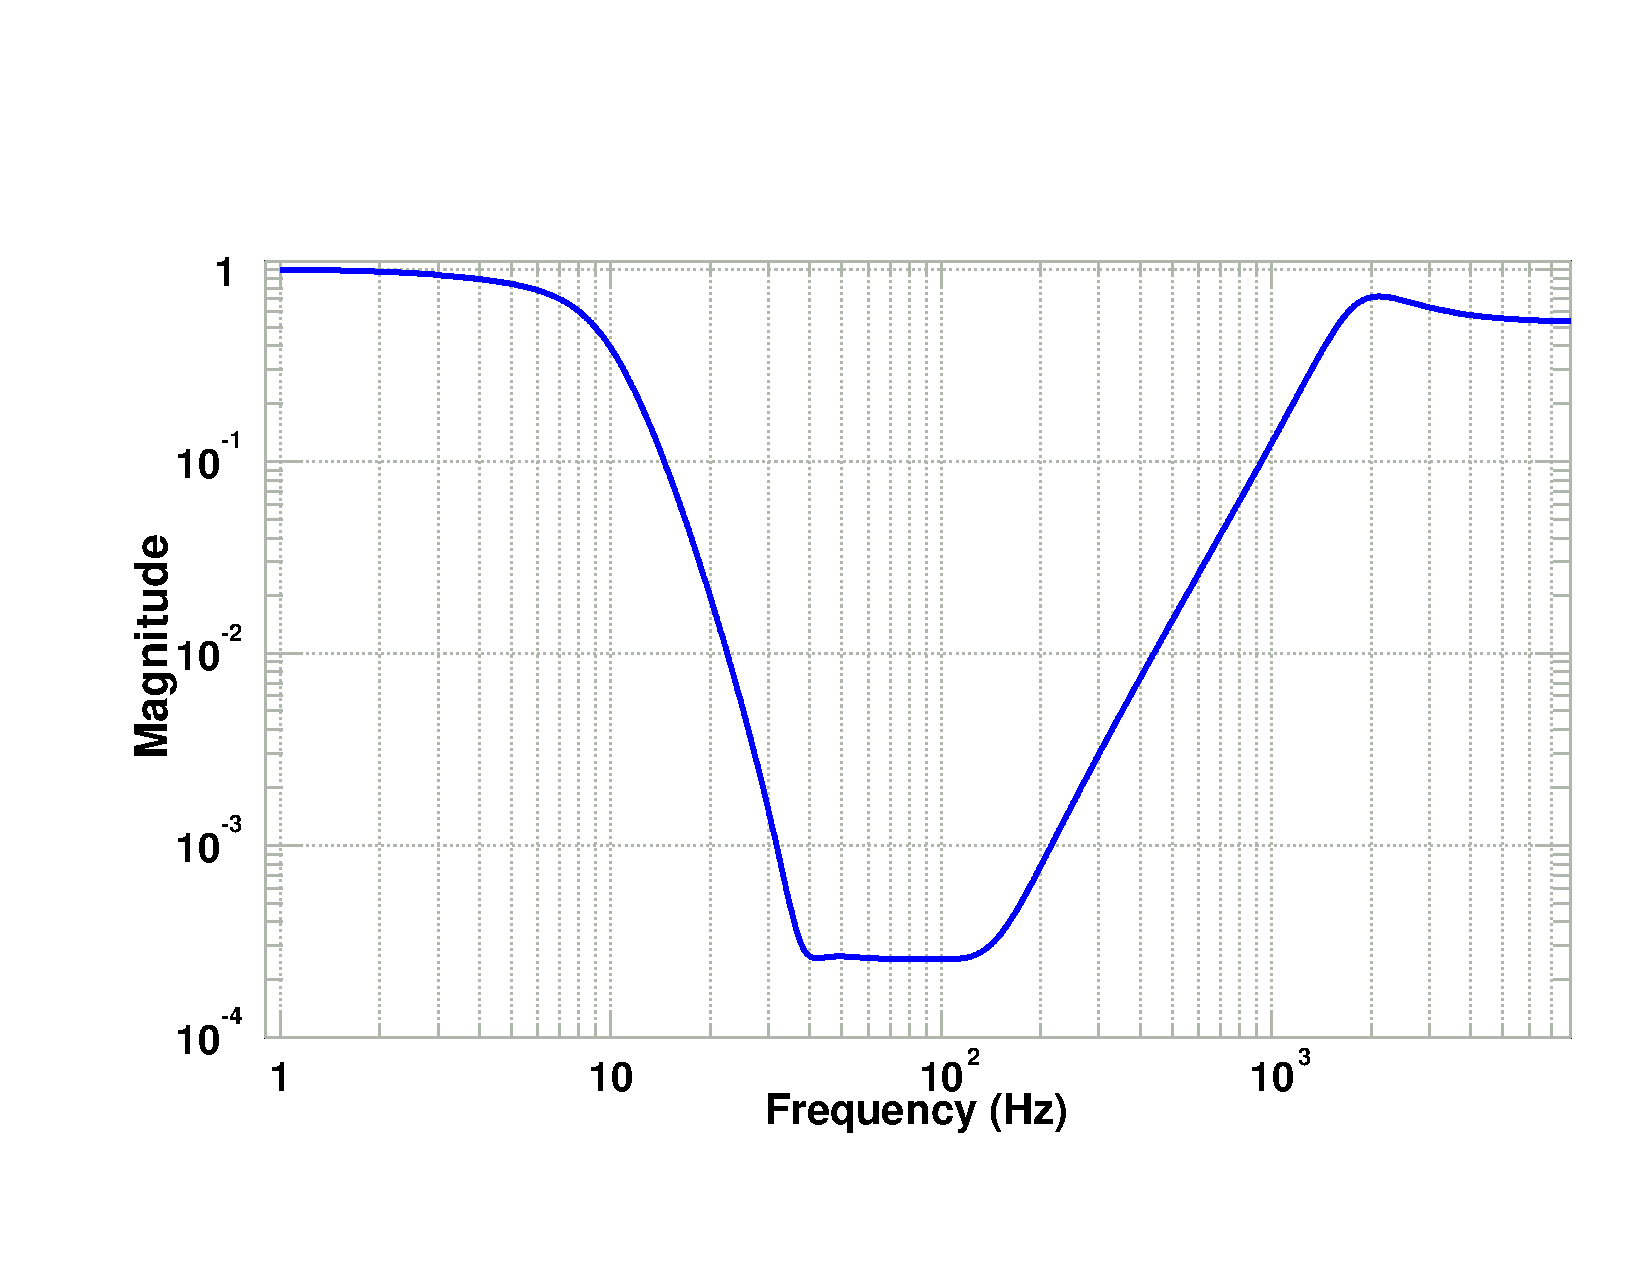
\includegraphics[angle=0,width=6.5in]{Figures/Chap4/dwf2.pdf}}
\caption[Dewhitening Filter]{Magnitude transfer function of the 
                             post-DAC dewhitening filter}
\label{fig:DWF}
\end{figure}
To keep the servo transfer function constant a digital inverse of
the analog filter is used to condition the signal before the DAC. There
is a potential for saturation in the DAC, due to the amplification in this
inverse filter. To reduce the dynamic range of the signal sent to the DAC,
the dewhitening filter is designed to only attenuate in the 40-150 Hz band
where the noise requirements are most critical.

\begin{figure}[!h]
\centerline{
\includegraphics[angle=0,width=6.5in]{Figures/Chap4/CoilNoise.pdf}}
\caption[DAC Noise]{A comparison of coil current noise from the electronics
         with the signal levels during S2. Also shown are the Johnson noise
         from a 3 k$\Omega$ resistor in series with the coil and the
         level of current noise required to meet the LIGO Science Requirement.}
\label{fig:OutputElectronics}
\end{figure}



%-------------------------------------------------------
\subsection{Angle to Length}

This section describes the mechanism for angular fluctuations of the optic to
affect the optical cavity length. The sources of angular fluctuations below
15~Hz are chiefly seismic. Above 15~Hz most of the angular noise comes from
the angular control servos (see Section~\ref{sec:ASC}).

The primary mechanism which couples angular noise into apparent length fluctuations
is the lever arm effect. If the beam is displaced from
the mirror's axes of rotation, a tilt will shift the phase of the entire beam
mimicking a length shift: $\delta x = d \, \tan{\theta}$, where $x$ is the translation
of the optic along the cavity axis, $d$ is the de-centering of the beam, and $\theta$
is the optic's rotation angle.

A second effect is cross-coupling of angular torque into piston motions of the optic
through imbalances in the magnets' dipole moments and the actuation electronics. 
The gravitational wave frequency band is far enough above the pendulum eigenfrequencies that 
we may treat the optic like a free mass. The torque applied by the control system is
$\mathfrak{T} = 4 F_c R/\sqrt{2}$, where $\mathfrak{T}$ is the torque, 
$F_c$ is the force per coil 
and $R$ is the radius of the optic. The displacement inducing force is 
$F_x = \alpha 4 F_c$, where $\alpha$ is the imbalance in the coils. The angle 
to length coupling may then be written as:

\begin{equation}
 \begin{aligned}
  \delta x &= \delta \theta \, \left [ \frac{F_x / m}{\mathfrak{T} / J} + d \right ]      \\
           &= \delta \theta \, \left [ \frac{\sqrt{2}}{4} \alpha 
               \left( R + \frac{H^2}{3 R} \right) + d \right ]
 \end{aligned}
\end{equation}
using the moment of inertia $J = \frac{1}{4} M R^2 + \frac{1}{12} M H^2$ for
a cylinder (see Figure~\ref{fig:SUS}).

In order to minimize the total noise, we adjust the coil gains individually to
minimize the overall angle $\rightsquigarrow$ length coupling for both pitch
and yaw rotations without regard to the actual mechanism. This method minimizes 
the noise at just one position on the mass, but can be done for whatever
position the beam is at. The alignment control system prevents long term
beam drift and so once optimized the noise should remain minimized.

The procedure to balance is to inject a sine wave into the 
pitch / yaw feedback path and then adjust the digital coil gains while reading 
back the response in the strain channel at the same frequency. We were able to 
automate this procedure and 
got an angle $\rightsquigarrow$ length coupling of 
$2 \times 10^{-4} \mbox{meters}/\mbox{radian}$; 
equivalent to a beam decentering of 0.2 mm or $\sim$0.3\% of a beam diameter. 
This level of balancing requires adjusting the coil gains at the 0.5\% level.

The obvious drawback to this method is that it does not actually center the
beam on the optic. Decentering can increase the sensitivity to thermal noise
in the suspensions angular eigenmodes (more on centering in Section \ref{sec:sweetspot}).

This method was not in place for the S2 run and so there the coupling was significantly
worse, $\approx0.1 \, \mbox{meters}/\mbox{radian}$.




%- - - - - - - - - -  -  -  - - - - - - -  -  -  -   -   -    -    -     -      -
%- - -  SENSING  NOISES- - - - - - -  -  -  -   -   -    -    -     -      -
%- - - - - - - - - -  -  -  - - - - - - -  -  -  -   -   -    -    -     -      -
\section{Sensing Noises}

Sensing noise includes noise which comes in on the laser, noise generated in the
interferometer (scattering), noise in the readout electronics, and shot noise from
the quantum statistics of the photons at the AS port. 


%-------------------------------------------------------
\subsection{Laser Amplitude Noise}
\label{sec:IntensityNoise}

Laser amplitude noise has three coupling mechanisms:

\begin{itemize}
\item Power fluctuations in the arms can produce differential lengths changes
      in the arm cavities if there is an imbalance in the stored power or
      the masses of the mirrors. As discussed above in 
      Section~\ref{sec:radpress}, this effect is negligible.

\item Power fluctuations in the mode cleaner can produce laser frequency
      noise through radiation pressure induced displacements of the low mass
      ($\sim$0.25 kg) MC mirrors. This is described in more detail in
      Appendix~\ref{app:ModeCleaner}.

\item Power fluctuations at the anti-symmetric port modulate the gain of
      the strain readout channel. Low frequency arm length fluctuations
      are upconverted into the gravitational wave band through this 
      amplitude modulation.
\end{itemize}
An input beam with low frequency amplitude modulation can be written as:

\begin{equation}
E_{in} = E_{0} \left(1 + \frac{\Delta A}{A} \right) \cos{\omega t} 
\end{equation}
where $A$ is the amplitude of the unmodulated laser light. The noise signal
in AS\_Q will by the multiple of two time series: $\delta G(t) \delta L_{-}(t)$. $G(t)$
is the optical gain at the AS port and $\delta L_{-}(t)$ is the $L_{-}$ servo's error point.

The coupling to the anti-symmetric port signal can be written as \cite{Sigg:FreqResp}:

% Intensity Noise Coupling
\begin{equation}
S_{\mbox{\tiny AS\_Q}} =
\aleph \, g_{cr} t_{sb} r_{c}' 
\left\{k \Delta L_{-} * 
\left[\frac{\Delta A}{A} 
\left(1 + \frac{1}{(1 + i f/f_{cc})(1 + i f/f_{c})}
\right) 
\right] 
\right\}
\label{eq:Intensity}
\end{equation}
where $*$ is the convolution of Fourier transforms of the two time series.
Above the double cavity pole, $f_{cc}$, the carrier fluctuations are filtered out
and so the optical gain modulation  comes from the amplitude noise on the RF sidebands which
travel unfiltered to the AS port.

Since laser amplitude noise is usually characterized by measurements of the power,
it is convenient to note that $2 \Delta A/A = \Delta P/P$. Another commonly
used expression for the power fluctuations is the Relative Intensity Noise (RIN)
which is equal to $\delta P_{rms}(f)/ P$.

Combining Equations \ref{eq:Intensity} and \ref{eq:darm2asq} we get
the apparent differential arm signal due to laser power fluctuations:

\begin{equation}
\delta L_{-}(f) = 5 \times 10^{-21} 
               \left[\left(\frac{\mbox{RIN}(f)}{1 \times 10^{-7}}\right) *
               \left(\frac{\Delta L_{-}(f)}{1 \times 10^{-13} \mbox{m}}\right)\right]
               \left(1 + \frac{f}{f_c}\right) \frac{\mbox{m}}{\sqrt{\mbox{Hz}}}
\end{equation}
Measurements of the intensity noise coupling have revealed that this bilinear
coupling term is dominated by a (currently) unexplained linear coupling which
is the equivalent of having a static $\Delta L_- \simeq 3 \times 10^{-13} \mbox{m}$.


%-------------------------------------------------------
\subsection{Laser Frequency Noise}
\label{sec:FreqNoise}

Fluctuations in the frequency of the laser can couple into
the interferometer's differential strain readout through imperfections in
the optics. The frequency noise of the laser is intrinsically limited by
spontaneous emission from the upper state into the laser mode. The spectral
density of the frequency fluctuations is given by
% Schawlow-Townes formula for laser frequency noise
\begin{equation}
\nu(f) = \frac{1}{2 \pi \, \tau_{st}} \sqrt{\frac{h\nu}{P_{laser}}} 
\end{equation}
which is a form of the Schawlow-Townes limit\cite{Yariv,Peter:YAG}.
Substituting parameters for the LIGO master oscillator give 
$\nu(f) \approx 30 \, \mbox{mHz}/\sqrt{\mbox{Hz}}$. In reality, the frequency noise
is dominated by technical noise (thermal, acoustic, electronics) below 100 kHz.

To achieved the necessary frequency stability the laser frequency fluctuations are 
suppressed by several stages
of active stabilization. This frequency stabilization scheme is detailed in
Section~\ref{sec:CMservo}. The following paragraphs mainly detail how the
unsuppressed frequency noise can couple into the strain readout.

Although there are multiple mechanisms for frequency noise to show up 
at the AS port, they have a common theme: an imbalance between the 
two arms of the interferometer spoils the otherwise perfect 
subtraction of laser noise.

To calculate the signal due to frequency noise, we write the 
laser frequency, $f$, as $f = f_{0} + \delta\! f_N cos(\omega t)$. 
Then the signal at the anti-symmetric port due to frequency noise is

% Frequency Noise Coupling Equation
\begin{equation}
 \begin{split}
S_{\mbox{\tiny AS\_Q}} = 
\aleph \, g_{cr} t_{sb} \frac{\delta\! f_N}{2 f} [
& 8 \pi \, r_{c} \frac{f_{c}l_{m}}{c} \frac{f}{f_{c}}
\frac{1 + i f / f_{c}}{1 + i f / f_{cc}} \\
+ &\frac{\delta f_{c}}{f_{c}} (1-r_{c}) 
\frac{f / f_{c}}{(1 + i f / f_{cc})(1 + i f / f_{c})} \\
+ &\delta r_{c} \frac{f / f_{cc}}{1+if /f_{cc}} ]
 \end{split}
\end{equation}
The first term in the above equation comes from the Schnupp asymmetry, 
$l_{-} \approx$ 175 mm. The audio-frequency, frequency noise sidebands on the
carrier light get different phase shifts in the two Michelson arms and so they 
do not perfectly cancel out at the AS port. This residual field beats with the
static sideband fields to produce a signal.

The second term is proportional to $\delta f_{c}/f_{c}$, the fractional
difference in the two arm cavity poles. For the 4 km arm cavities, 
$f_{c} \approx $ 85 Hz and the fractional difference has been
measured by cavity ringdown to be $\sim$2\% (see Appendix \ref{app:optics}). 
A mismatch in the arm cavity poles
comes about through a difference in the round-trip loss (including mirror
transmissions). The loss in the arms
is dominated by the $\sim$3\% transmission of the input test masses. Note that since
the end mirrors have a reflectivity of $\sim$1, an arm cavity with no internal
scatter loss or absorption will still have an overall reflectivity of $\sim$1. So
the carrier fields reflected from the two arms have the same amplitude, but
different phase. At frequencies above the arm cavity pole the carrier audio
sidebands do not resonate in the arms and so do not experience a differential
phase shift from the cavity pole imbalance. Therefore the frequency noise
coupling due to the arm cavity pole imbalance gets smaller above the arm cavity pole.

The third term in the equation is somewhat different and is, in practice,
the dominant effect. At frequencies
above the coupled cavity pole, the carrier's audio sidebands are filtered off
but the audio sidebands of the RF sidebands couple directly to the AS port.
In a perfect interferometer this would have no effect, but an imbalance in
the reflectivity of the arm cavities will produce a static, TEM$_{00}$ carrier
field at the AS port. Since the differential arm servo loop only suppresses
differential phase shifts, this static field is not nulled. The audio sidebands
of the RF sidebands then beat against this static carrier to produce a signal
in AS\_Q.

As shown in Figure~\ref{fig:FreqNoise}, the term from the reflectivity
imbalance is dominant. For typical parameters at frequencies above the arm
cavity pole the apparent displacement noise from frequency noise is:

\begin{equation}
\delta L_{-}(f) \simeq 3.5 \times 10^{-20} 
                  \left(\frac{\delta r_c}{5 \times 10^{-3}}\right)  
             \left(\frac{\delta f_N}{1 \times 10^{-6} \, \mbox{Hz}/\sqrt{\mbox{Hz}}}\right)
                  \frac{\mbox{m}}{\sqrt{\mbox{Hz}}}
\end{equation}

\begin{figure}[!h]
\centerline{
\includegraphics[angle=0,width=6.5in]{Figures/Chap4/FreqNoiseCoupling.pdf}}
\caption[Frequency Noise Couplings]{Shown are the three frequency noise
         coupling mechanisms. Asymmetries: $l_-$ = 175 mm,
         $\delta f_{c} = 2 \, \mbox{Hz}$, $\delta r_{c}$ = 0.5 \%}
\label{fig:FreqNoise}
\end{figure}
A reflectivity imbalance comes about through
a difference in the losses of the two arms. A full description of the 
optics' characterization is in Appendix~\ref{app:optics},
but stated simply, we know from the power buildup in the interferometer that
the scatter loss ($\approx$70 ppm/mirror) is more important than the ETM transmission
($\sim$10 ppm). 



%-------------------------------------------------------
\subsection{Oscillator Amplitude Noise}

A commercial signal generator (IFR 2023A) is used to generate the modulation
waveform for the resonant RF sidebands. The output of the oscillator is
multiply split; several outputs are used to power the local oscillator
input of the various mixers used to demodulate the RF signals from the
detection ports.

One output of the splitter is actively amplitude stabilized and then used
to drive a phase modulator (see Section~\ref{app:IOO}).
Residual fluctuations in the modulation amplitude lead to sideband
amplitude fluctuations. Noise on the amplitude of the sidebands
modulates the optical gain at all of the readout ports. The RF mixers 
which demodulate the RF signal from the photodiodes are driven to
saturation on the Local Oscillator (LO) port and so there is no sensitivity 
to amplitude fluctuations of the LO drives. 
Oscillator amplitude noise shows up as \cite{Sigg:FreqResp}

\begin{equation}
S_{\mbox{\tiny AS\_Q}} =
\aleph g_{cr} t_{sb} r_{c}' \frac{\Delta \Gamma}{\Gamma} \, k \Delta L_{-}
\end{equation}
where $\Gamma$ is the modulation depth in radians. At frequencies
above the arm cavity pole, for typical parameters we get:

\begin{equation}
\delta L_- \simeq 1 \times 10^{-19}
           \left(\frac{\Delta \Gamma(f) / \Gamma}{1 \times 10^{-7} /\sqrt{\mbox{Hz}}} \right)
           \left(\frac{f}{1 \, \mbox{kHz}} \right)
           \left(\frac{\Delta L_-}{1 \times 10^{-13} \mbox{m}_{\mbox{\tiny RMS}}} \right)
           \frac{\mbox{m}}{\sqrt{\mbox{Hz}}}
\end{equation}
The amplitude noise of the oscillator has been measured to be just below
10$^{-7}$ from 100-1000 Hz and falling rapidly above 1 kHz.



%-------------------------------------------------------
\subsection{Oscillator Phase Noise}

Another noise source is phase jitter on the oscillator. So far the exact
coupling mechanism of oscillator phase noise has not been determined
but measurements have been made which show that it is currently a limiting
noise source and so it pays to speculate about the coupling mechanism in
order to have some theory to test.

In principle, there is no first order coupling of oscillator phase noise
to the dark port since any noise is common to both the signal and the local
oscillator and is therefore canceled
in the demodulated signal. Relative phase lags in the two paths between
the oscillator and the mixer break this symmetry and can produce a sensitivity
to phase noise.

There are 3 main sources of phase lag:
\begin{itemize}
\item Relative path length differences lead to an overall time delay. The
      difference is $\sim30$ m. Although this gives a substantial
      phase shift at the modulation frequency, once this is compensated
      for (by e.g. a length of cable) the remaining phase shift at audio
      frequencies around the carrier are negligible: $\sim10^{-4}$ radians
      at 1 kHz.

\item The power recycling cavity has a pole frequency of 
      $\approx170 \mbox{kHz}$. This filters the phase noise on the
      optical RF sidebands, but does not affect the local oscillator
      and so makes a small differential phase shift proportional to
      $f$/(170 kHz) below the recycling cavity pole.

\item The dominant phase shift for the optical RF sidebands comes from the 
      mode cleaner which acts as a $\approx4$ kHz low pass filter on the
      phase noise.
\end{itemize}

Oscillator phase noise can be represented by modifying the expression
for the input field:

\begin{equation}
E_{in} =
E_{0} e^{i \Gamma cos(\omega_{m}t + \phi_{N} cos \omega_{a} t)}
\end{equation}
In principle, even with this asymmetry there would be no coupling. In
both the symmetric and anti-symmetric ports, however, there is a large
unsuppressed signal in the demodulation phase quadrature which is not
used in the interferometer length control (REFL\_Q \& AS\_I, respectively).
These large low frequency signals get mixed into the signal phase by the
fractional phase angle difference between the LO and RF paths.

The signal at the anti-symmetric port due to this signal can be written as:

\begin{equation}
S_{\mbox{\tiny AS\_Q}} =
S_{\mbox{\tiny AS\_I}} \frac{i f /f_{\mbox{\tiny MC}}}{1 + i f /f_{\mbox{\tiny MC}}} 
                       \phi_N(f) 
\end{equation}
The particular model of signal generator (IFR 2023A w/ option 14)
used to generate the modulation waveform was chosen because of its
low phase noise spectrum (-130 dBc/$\sqrt{\mbox Hz}$). Custom built 
quartz oscillators having phase noise as low as -160 dBc/$\sqrt{\mbox Hz}$ 
can be purchased, although the commercial signal generator allowed the kind
of frequency tuning flexibility which is outside the range of the
quartz oscillators. 

If it is true that the coupling mechanism depends on the amplitude of the
AS\_I signal, future reductions of the signal in this quadrature would also 
reduce the oscillator phase noise contribution to the strain sensitivity.



%-------------------------------------------------------
%\subsection{Scattering}
%
%Scattered light in the interferometer which returns to the anti-symmetric
%port photodetector can cause spurious signals. Some things which scatter:
%
%\begin{itemize}
%\item Rayleigh scattering off of the residual gas particles in the
%      long beamtubes. 
%
%\item Light which scatters unintentionally somewhere within the interferometer
%      and then returns to the main beam path can modulate the field at the
%      detection ports. Great care has been taken in the in-vacuum optical
%      layout to control all extra reflections of a significant level.
%      Backscattering of this type limits the sensitivity at the symmetric
%      port (see Section~\ref{sec:CMscatter}).
%\end{itemize}
%
%\subsubsection{Residual Gas}
%
%The scattering due to residual gas particles has the form \cite{Mike:Gas,Rai:Scattering}:
%
%\begin{equation}
%\delta L_{-}(f) = 4 \pi \alpha 
%      \sqrt{\frac{\rho}{v_{0}}\int\nolimits_{0}^{L_{0}}
%      \frac{exp[-2 \pi f w(z)/v_{0}]}{w(z)} \, dz}
%\end{equation}
%where $v_{0}$ is the mean particle speed, $w(z)$ is the beam radius,
%$\rho$ is the number density, and $\alpha$ is the polarizability.
%(need to get parameters for H2, H20, hydrocarbons)
%
%The noise from residual gas scattering is expected to be insignificant at
%our designed strain sensitivity level, due to very low pressure (column
%density) of the gas in the beam tubes.


\subsection{Beam Clipping on the Optical Tables}

As the sensitivity in the interferometers improved, it became clear that there
is a great deal of sensitivity to the acoustic noise on \emph{every} optical table.

This acoustic sensitivity comes about through clipping of the beam on the
optical table through apertures and dusty optics. A hypothesis is that
the large diameter junk fields, from the contrast defect for the carrier or
the instability of the recycling cavity for the sidebands, produce
a signal when clipped. The aperturing of the higher order fields produces
some light which overlaps with the TEM$_{00}$ mode to produce a signal. 

This is largely reduced by enforcing the standard practices
of cleanliness, careful alignment, and dumping of secondary beams (into beam
dumps which are dark at 1 micron). This type of noise is what was
mainly responsible for the 100-1000 Hz structure in the H1 and H2 curves in
Figure~\ref{fig:S2noiseComp}. It has been greatly reduced by the installation
of an acoustic isolation enclosure around the AS port tables
of each interferometer and by the use of larger optics on the table.



%-------------------------------------------------------
\subsection{Auxilliary Length Controls}
\label{sec:POBnoise}

Fluctuations of lengths other than the differential arm cavity
degree of freedom can produce signals at the Anti-Symmetric port. The average
length of the arm cavities is not controlled at most frequencies
but is tracked by the laser as described in Section~\ref{sec:CMservo}.

The other two lengths, $l_{-}$, the differential mode of the recycling
cavity and $l_{+}$, the common mode of the recycling cavity, produce
AS port signals in very different ways.

\begin{equation}
 \begin{split}
  \delta L_{-}(f) &= \frac{r_{c}}{r_{c}'} \delta l_- \\
                  &\simeq \frac{1}{140} \delta l_-
 \end{split}
 \label{eq:mich2darm}
\end{equation}
The $l_{-}$ coupling is straightforward; it is described by
Equation~\ref{eq:mich2asq}. The mechanism is similar to the way 
the differential arm signal is generated, the difference being that 
the $l_{-}$ signal does not get amplified by the arm cavity finesse.

\begin{equation}
 \begin{split}
  \delta L_{-}(f) &= 2 \delta r_{c} \frac{1}{r_{c}'} 
                     \frac{g_{sb} r_{M}}{t_{RM} t_{M}}
                     \delta l_{+} (1 + i f / f_c) \\
           &\simeq \frac{1}{1400} \delta l_{+} (1 + i f / f_c)
 \end{split}
 \label{eq:prc2darm}
\end{equation}
The $l_{+}$ coupling turned up unexpectedly in the course of 
commissioning. It is produced in a similar way to laser 
frequency noise coupling: audio sidebands on the RF sidebands beat with a 
static carrier at the AS port to produce an audio frequency signal. 
In this case, the audio sidebands are created by modulation of 
the $l_{+}$ length. The static carrier is produced by a reflectivity
imbalance between the two arms, same as frequency noise coupling.

\begin{figure}[!h]
\centerline{
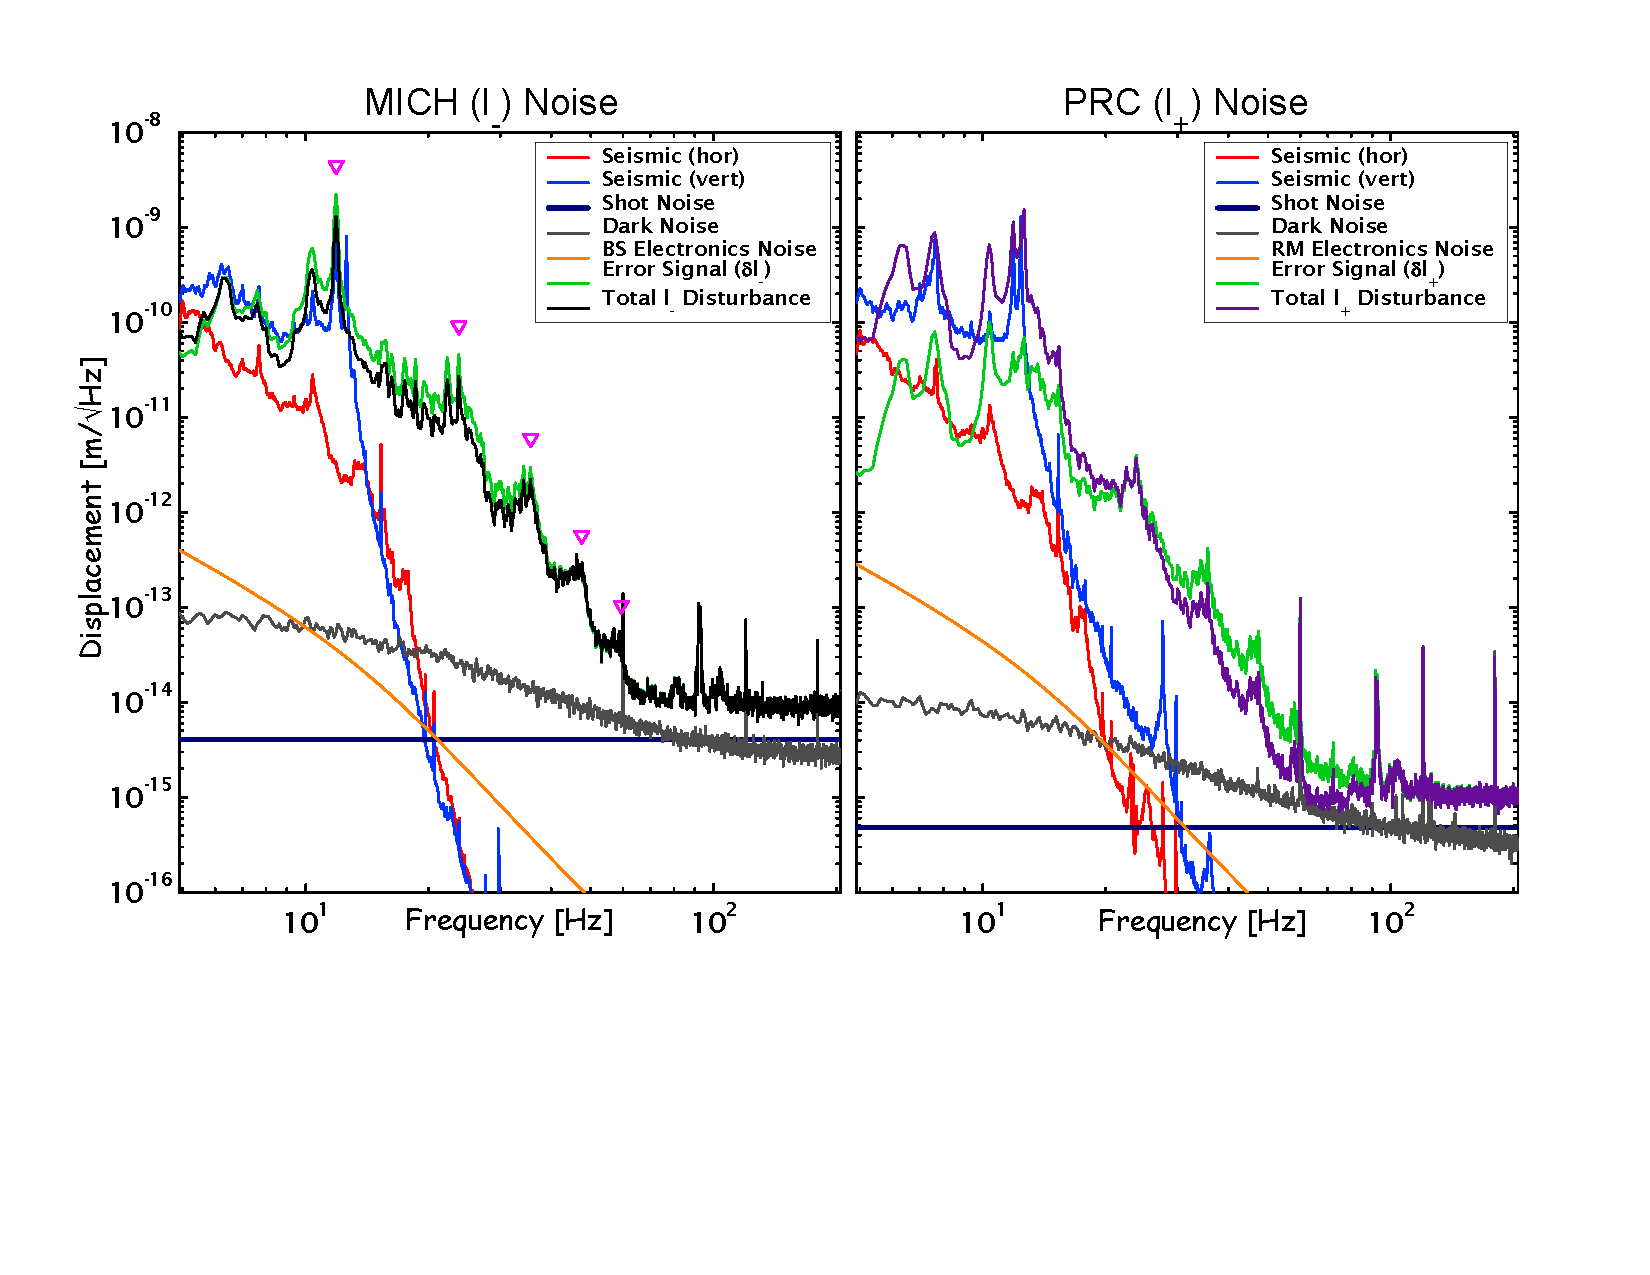
\includegraphics[angle=0,width=6.5in]{Figures/Chap4/POBnoise.pdf}}
\caption[POB Noises]{The two plots show the displacement
         spectra for both of the recycled Michelson DOFs; MICH ($l_-$) 
         \& PRC ($l_+$) and their known contributing noise sources.
         The triangles on the MICH plot indicate the harmonics of
         suspended optic's vertical bounce mode.}
\label{fig:POBnoise}
\end{figure}

Both of these lengths must be controlled in order to keep the interferometer
resonating. The length controls servos' gain must also be high enough
that the residual fluctuations of these lengths do not compromise the
strain sensitivity (more on this in \ref{sec:LSC}).

The largest disturbance to these lengths comes from seismic noise. As
shown in the plots, the dominant contribution is from vertical noise.
The 'vertical noise' traces actually refer to the apparent cavity
length fluctuations which arise from vertical motion of the optic.

The coupling is much larger for the recycling cavity than for the
arm cavities. In this case, the $\sim$1 degree vertical wedge angles
are the main coupling source. The exact positions and angles
of each optic surface are documented \cite{Dennis:WedgeAngles}. The
'vertical noise' trace is estimated by first measuring the vertical
motion with an accelerometer mounted external to the vacuum chamber.
This trace is converted into displacement units, multiplied by
the modeled vertical $\Rightarrow$ vertical transfer function of the 
stack, and then multiplied by the vertical $\Rightarrow$ vertical transfer function 
of the pendulum suspension which takes into account the compliance 
of the steel suspension wire.

This is done separately for each of the four recycling cavity masses and
then summed with the appropriate geometrical factors to make the displacement
noise.

In principle, the only other noise limit to these lengths should be
in the sensing chain. The dark noise curve in Figure~\ref{fig:POBnoise}
is the result of ADC noise below 100 Hz and the noise of the photodetector
above 100 Hz. The shot noise limited displacement sensitivity of these
degrees of freedom is rather high compared to the Anti-Symmetric or
Reflected ports; only a small fraction
of the circulating field  in the recycling cavity is picked-off for the 
signal detection.

It is clear from these plots, that the normal linear coupling mechanisms
are not good enough to predict the noise that we actually see. The 
indicators in the MICH plot of Figure~\ref{fig:POBnoise} show what appears
to be significant upconversion of the large amplitude low frequency 
motions, implying that the bilinear noise mechanism has, as one of its
terms, the vertical bounce mode.



%-------------------------------------------------------
\subsection{Shot Noise}
\label{sec:ShotNoise}

Vacuum field fluctuations entering the interferometer through the
anti-symmetric port affect the interferometer's phase sensitivity
by beating with the RF sidebands~\cite{Caves:RadPress,Caves:Squeezing}. 
This is often described
as 'shot noise': Poisson arrival time statistics of the light
on the photodetector.

In addition to this more fundamental noise source, there is also extra
shot noise introduced by the presence of junk light on the photodiode.
The differential arm signal is in principle only dependent on
the amount of light in the TEM$_{00}$ mode but the shot noise level
depends on the total light level since the light power level is not
dominated by the beat between the carrier and sideband fields.

The expression for the shot noise signal at the AS port is\cite{Sigg:FreqResp}:

\begin{equation}
S_{\mbox{\tiny AS\_Q}} =
2 \sqrt{[J_0(\Gamma)^2 g_{cr}^2 c_d 
       + \frac{3}{2} 2 J_1(\Gamma)^2 t_{sb}^2] P_{in} h \nu}
\label{eq:ShotNoise}
\end{equation}
where $c_d \equiv P_{AS}/P_{BS}$ is the carrier contrast defect. 
The two terms in the bracket are essentially 
just the carrier power 
($\propto J_0(\Gamma)^2$) and the sidebands' power ($\propto J_1(\Gamma)^2$). The
factor of 3/2 in the term for the sidebands' power derives from the non-stationary
nature of the shot noise produced by the 
sidebands~\cite{Niebauer:ShotNoise} and the fact that we are using
effectively a sine wave demodulation~\cite{Meers:modulation}.
Combining Equations \ref{eq:darm2asq} and \ref{eq:ShotNoise} gives us an 
expression for the equivalent differential arm length noise:

\begin{equation}
\delta L_- \simeq 3.6 \times 10^{-17} \sqrt{\frac{1}{P_{in}}}
            \frac{\sqrt{J_0(\Gamma)^2 g_{cr}^2 c_d 
                     + \frac{3}{2} 2 J_1(\Gamma)^2 t_{sb}^2}}
                 {J_0(\Gamma) J_1(\Gamma) g_{cr} t_{sb} r_{c}'}
             \left(1 + i \frac{f}{f_c}\right)
            \frac{\mbox{m}}{\sqrt{\mbox{Hz}}}
\end{equation}
We can then optimize the SNR, by adjusting the modulation depth, $\Gamma$,
to minimize this function.


\subsubsection{Mode Overlap and Optical Gain}

The above formula and all of the formulae in Chapter~\ref{chap:signals}
are valid in the limit that all of the light is in the same spatial
mode. This is not exactly true at any port; the situation at the
Anti-Symmetric port is of the most concern.

The differential arm strain signal is encoded on the carrier light
returning to the beamsplitter as a differential phase shift. After
interfering at the beamsplitter a small field proportional to this
phase difference comes out of the AS port. The spatial
profile of this signal field is set by the \emph{average} of the
resonant modes in the two arm cavities. If the arms
are well matched spatially, this is not a significant distinction
to make.

What is significant is the spatial mode of the RF sidebands at the
AS port. Due to the spatial mismatch between the
recycling cavity 'mode' and that of the arm cavities
(see Section~\ref{sec:ThermalComp} for details), some fraction
of the sideband field at the AS port contributes to making
shot noise but not to the signal gain.

Nominally, the length signal, AS\_Q, is not sensitive to the higher
order spatial modes except as it relates to the generation of shot noise.
This is because a higher order TEM$_{mn}$ mode is orthogonal to the
nominally TEM$_{00}$ local oscillator field of the RF sidebands.
However, the presence of higher order modes in both the sidebands and
carrier will contribute directly to the signal (some in AS\_I
and some in AS\_Q). This signal is nulled in the I-phase quadrature
with the AS\_I servo (see Section~\ref{sec:Gorilla}), but in the
Q-phase this signal has to be nulled by introducing a differential
arm length offset.



%-------------------------------------------------------
\subsection{Readout Electronics}

Another technical source of noise is the electronics chain which reads
out the strain signal. The following block diagram shows the signal flow:

\begin{figure}[!h]
\centerline{
\includegraphics[angle=0,width=6.5in]{Figures/Chap4/SensingChain.jpg}}
\caption[Sensing Electronics]{Shows the signal flow from the RF photodiode to
         the analog-to-digital (ADC) converter.}
\end{figure}

Since the goal is to achieve the minimum strain noise possible we design
the electronics noise to be less than 1/10 of the noise coming from the more
fundamental shot noise.

To accomplish this, the signal-to-noise ratio achieved at the front end
electronics is not degraded throughout the chain into the ADC. The 
dark noise of the photodetector at the anti-symmetric port (described in 
more detail in Appendix~\ref{app:RFPD}) is in principle, \emph{dominated by the 
thermal noise of the LC resonant circuit formed by the photodiode and the inductor}.
So the requirement on the whitening electronics is only to increase the
signal from shot noise (or other 'fundamental' sources like thermal or seismic)
to at least 10X the ADC noise level. This is balanced by the desire to maintain 
a factor of 30 or more in headroom between the RMS signal level and the ADC input range.



%- - - NOISE NOISE NOISE NOISE - - - - - - -  -  -  -   -   -    -    -     -      -
\section{Some Notes about the Noise}

The interferometer noise is usually unexplained in several frequency bands and 
it is always changing (sometimes for the better). Therefore,
I have attempted here to give a good accounting of the noise as it was in
2002-2003, which were the years in which LIGO held its first three science runs
(creatively named S1, S2 \& S3).

\subsection{The Status of the Noise}

\begin{figure}[!h]
\centerline{
\includegraphics[angle=-90,width=6.5in]{Figures/Chap4/S3noise.pdf}}
\caption[S3 Noise]{Full Noise Budget for L1 during S3 (data from Dec. 23, 2003)}
\label{fig:S3noise}
\end{figure}
Figure~\ref{fig:S3noise} is a good summary of this entire chapter. The point of
doing all of the noise analysis and budgeting is to always know what noise
sources limit the interferometer sensitivity and how this noise can be reduced.
The traces in the plot are not all made in the same way. Some of the traces
(e.g. oscillator phase noise) are made by measuring the source of the noise
(oscillator phase noise) and then the transfer function to AS\_Q and then 
multiplying them. Other traces
(e.g. internal thermal noise) are almost entirely based on a model for the
noise with few measurements for support.

The noise will often fluctuate upwards by factors of a few due to short time
transients or instabilities in the control servos. These plots of the amplitude
spectral density do not capture this character.


\subsection{A Brief History of the Noise}

These interferometers actually 'awoke' with noise levels at least 5 orders
of magnitude higher. These next paragraphs attempt to give a short synopsis 
on the major developments between each noise epoch shown 
in Figure~\ref{fig:NoiseHist}.

\begin{figure}[!h]
\centerline{
\includegraphics[angle=-90,width=6.5in]{Figures/Chap4/NoiseHist.pdf}}
\caption[LLO Noise History]{Noise history of the Livingston Interferometer from
                            2001-2003.}
\label{fig:NoiseHist}
\end{figure}


\subsubsection{May 18$^{th}$, 2001}

Pre power-recycling. The RM is misaligned intentionally to allow locking of
the Fabry-Perot Michelson in an optically recombined but not recycled mode. 
In this configuration there is very little
light at the anti-symmetric port available for locking and so the noise above
1 kHz is dominated by the dark noise of the sensing electronics. The vast array
of line spikes at multiples of 60 Hz are from the switching power supplies which were
in use at this time. In addition, there is no feedback from the interferometer 
to suppress laser frequency noise which therefore dominates the noise from 80-500 Hz.


\subsubsection{December 12$^{th}$, 2001}

The vacuum system was vented over the summer of 2001 to allow a number of repairs:
several of the suspensions' local sensors had broken photodiodes, wires, etc. 
In addition this version of local sensor had a photodiode which was sensitive to 
the 1064 nm laser light. New sensor / actuator heads were installed on all optics 
which are more than 100X less sensitive at 1064 nm.


\subsubsection{December 21$^{th}$, 2001}

Lower DAC Noise: First successful attempts to run the interferometer with the 
post-DAC dewhitening filters.


\subsubsection{May 27$^{th}$, 2002}

Power recycling and frequency stabilization. The first part of this year
was spent increasing the robustness of the the power-recycled configuration. 
The common mode servo was installed in a preliminary configuration and gave some
suppression of the frequency noise.


\subsubsection{August 24$^{th}$, 2002  (S1 Science Run)}

Common mode servo was revamped: $L_+$ feedback to the arms was removed
and the CM feedback to the mode cleaner length was changed to use a digital
servo. At this point it was discovered that through some non-linear
mechanism the noise is AS\_Q around 100 Hz could be reduced by increasing
the differential arm loop gain at 10-20 Hz. This later turned out to be
large bilinear upconversion around the power line harmonics. The source
was never identified, but the noise went away in the next major 
electronics upgrade.


\subsubsection{March 6$^{th}$, 2003  (S2 Science Run)}

All the electronics for the suspension controls are replaced with a mostly digital 
system allowing for greater flexibility. The introduction of the AS\_I servo
made it possible to detect nearly all of the light at the anti-symmetric port.
The large shelf of noise at 35 Hz from the optical lever servos is finally
reduced by whitening the optical lever sensor signals before the ADC.


\subsubsection{December 24$^{th}$, 2003  (S3 Science Run)}

Very little broadband improvement in sensitivity. An acoustic enclosure
was installed over the anti-symmetric port optics table, greatly reducing the
acoustic noise susceptibility. Efforts to commission the wavefront sensor
based angular control system were only partially successful and most of the run
had only 8 out of 16 degrees of freedom under control; 6 more than in S2, but not
enough to greatly improve stability.

The noise improvements at low
frequencies came from improved filtering of the optical lever servos
and the Michelson control loops. One notable improvement is the addition
of an off diagonal drive in the length control which feeds a small
fraction of the $l_-$ control signal to the $L_-$ length. This was
implemented mid-run and greatly improved the character of the noise
in the 30-70 Hz region.


\begin{figure}[!h]
\centerline{
\includegraphics[angle=0,width=6.5in]{Figures/Chap4/S1noiseComp.pdf}}
\caption[S1 Noise Curves]{Comparison of the interferometer noises during the
           first Science Run (S1).}
\label{fig:S1noiseComp}
\end{figure}


\begin{figure}[!h]
\centerline{
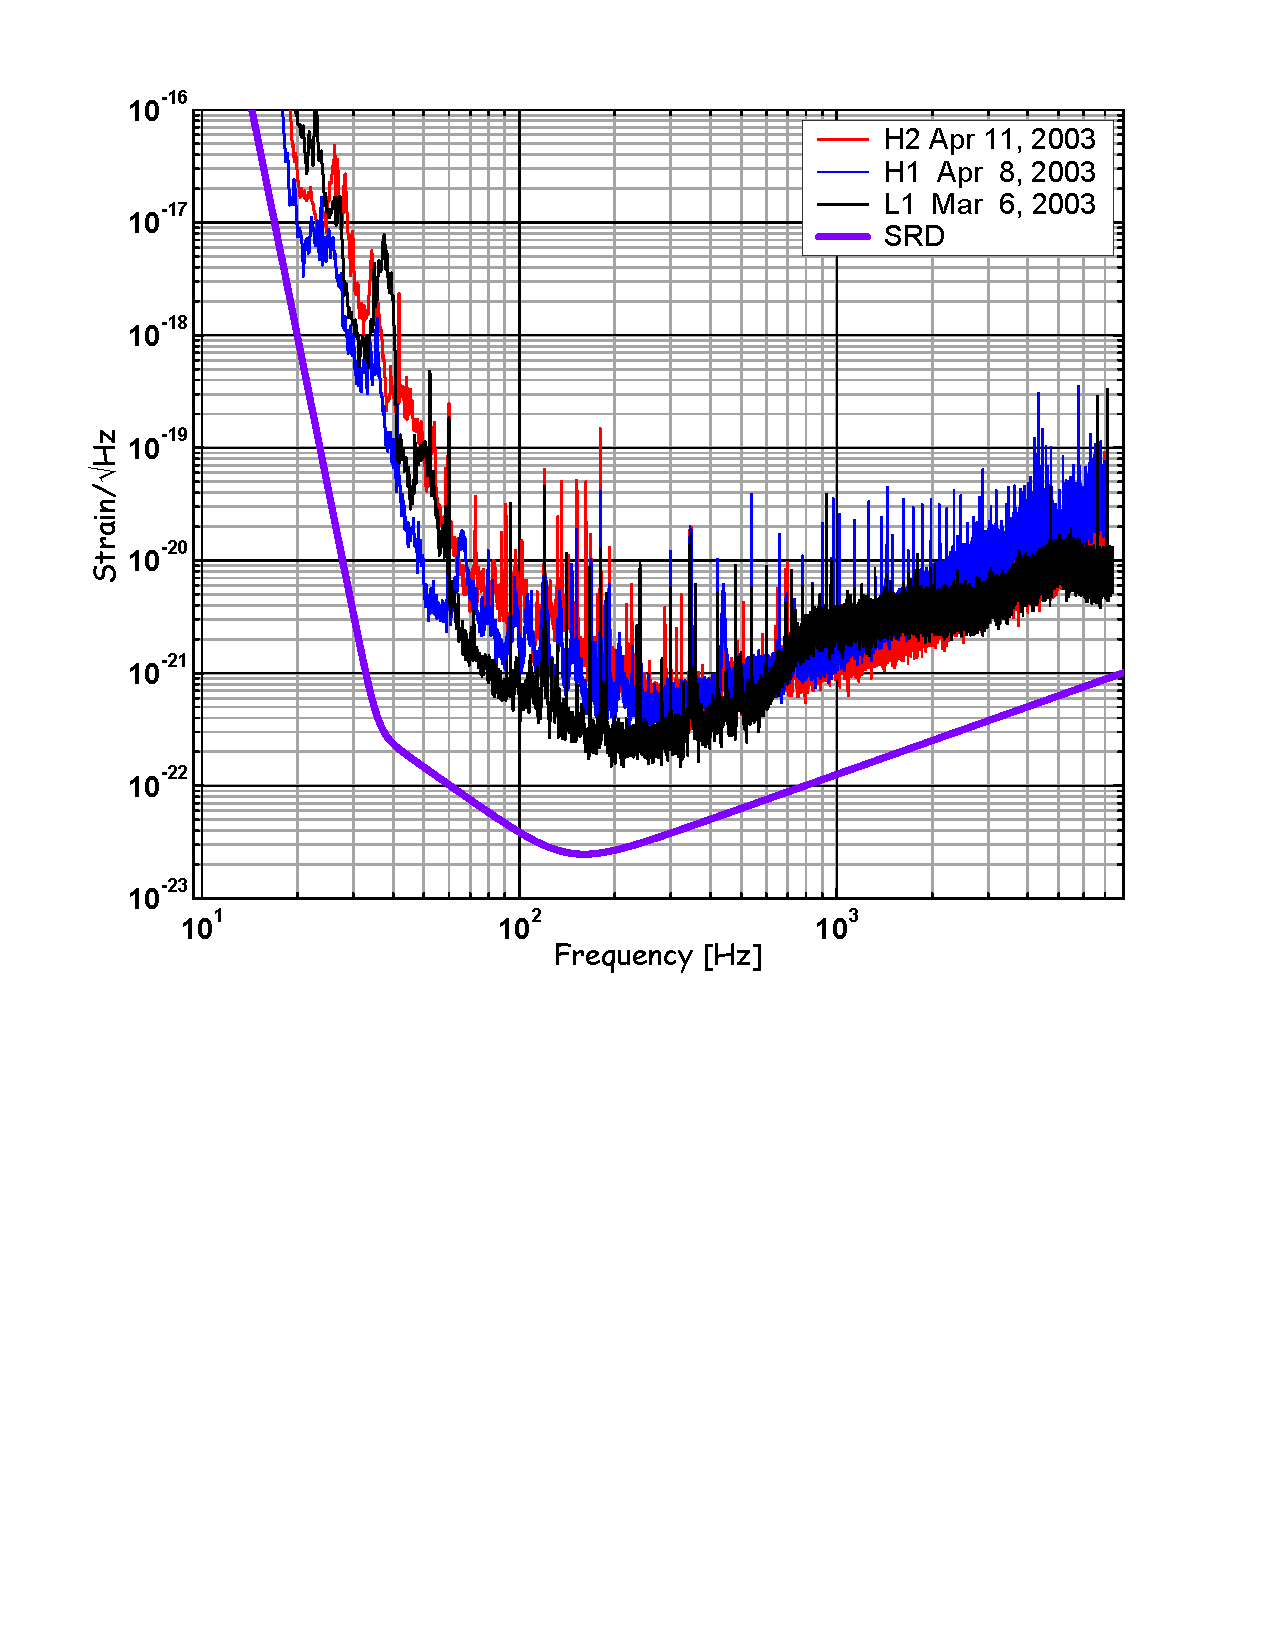
\includegraphics[angle=0,width=6.5in]{Figures/Chap4/S2noiseComp.pdf}}
\caption[S2 Noise Curves]{Comparison of the interferometer noises during the
           second Science Run (S2).}
\label{fig:S2noiseComp}
\end{figure}


\begin{figure}[!h]
\centerline{
\includegraphics[angle=0,width=6.5in]{Figures/Chap4/S3noiseComp.pdf}}
\caption[S3 Noise Curves]{Comparison of the interferometer noises during the
           third Science Run (S3).}
\label{fig:S3noiseComp}
\end{figure}


\subsection{Evolution of Phase Sensitivity}

The original Michelson interferometers were able to resolve
down to 1\% of an optical fringe. The LIGO sensitivity goal requires a phase
noise level of $3.5 \times 10^{-11}$ radians/$\sqrt{\mbox{Hz}}$. This very
small phase shift can be sensed due mainly to the increased power levels
in the Michelson part of the interferometer. Figure~\ref{fig:PhaseNoise}
shows the evolution of optical phase noise measurements in the last 40 years.

\begin{figure}[!h]
\centerline{
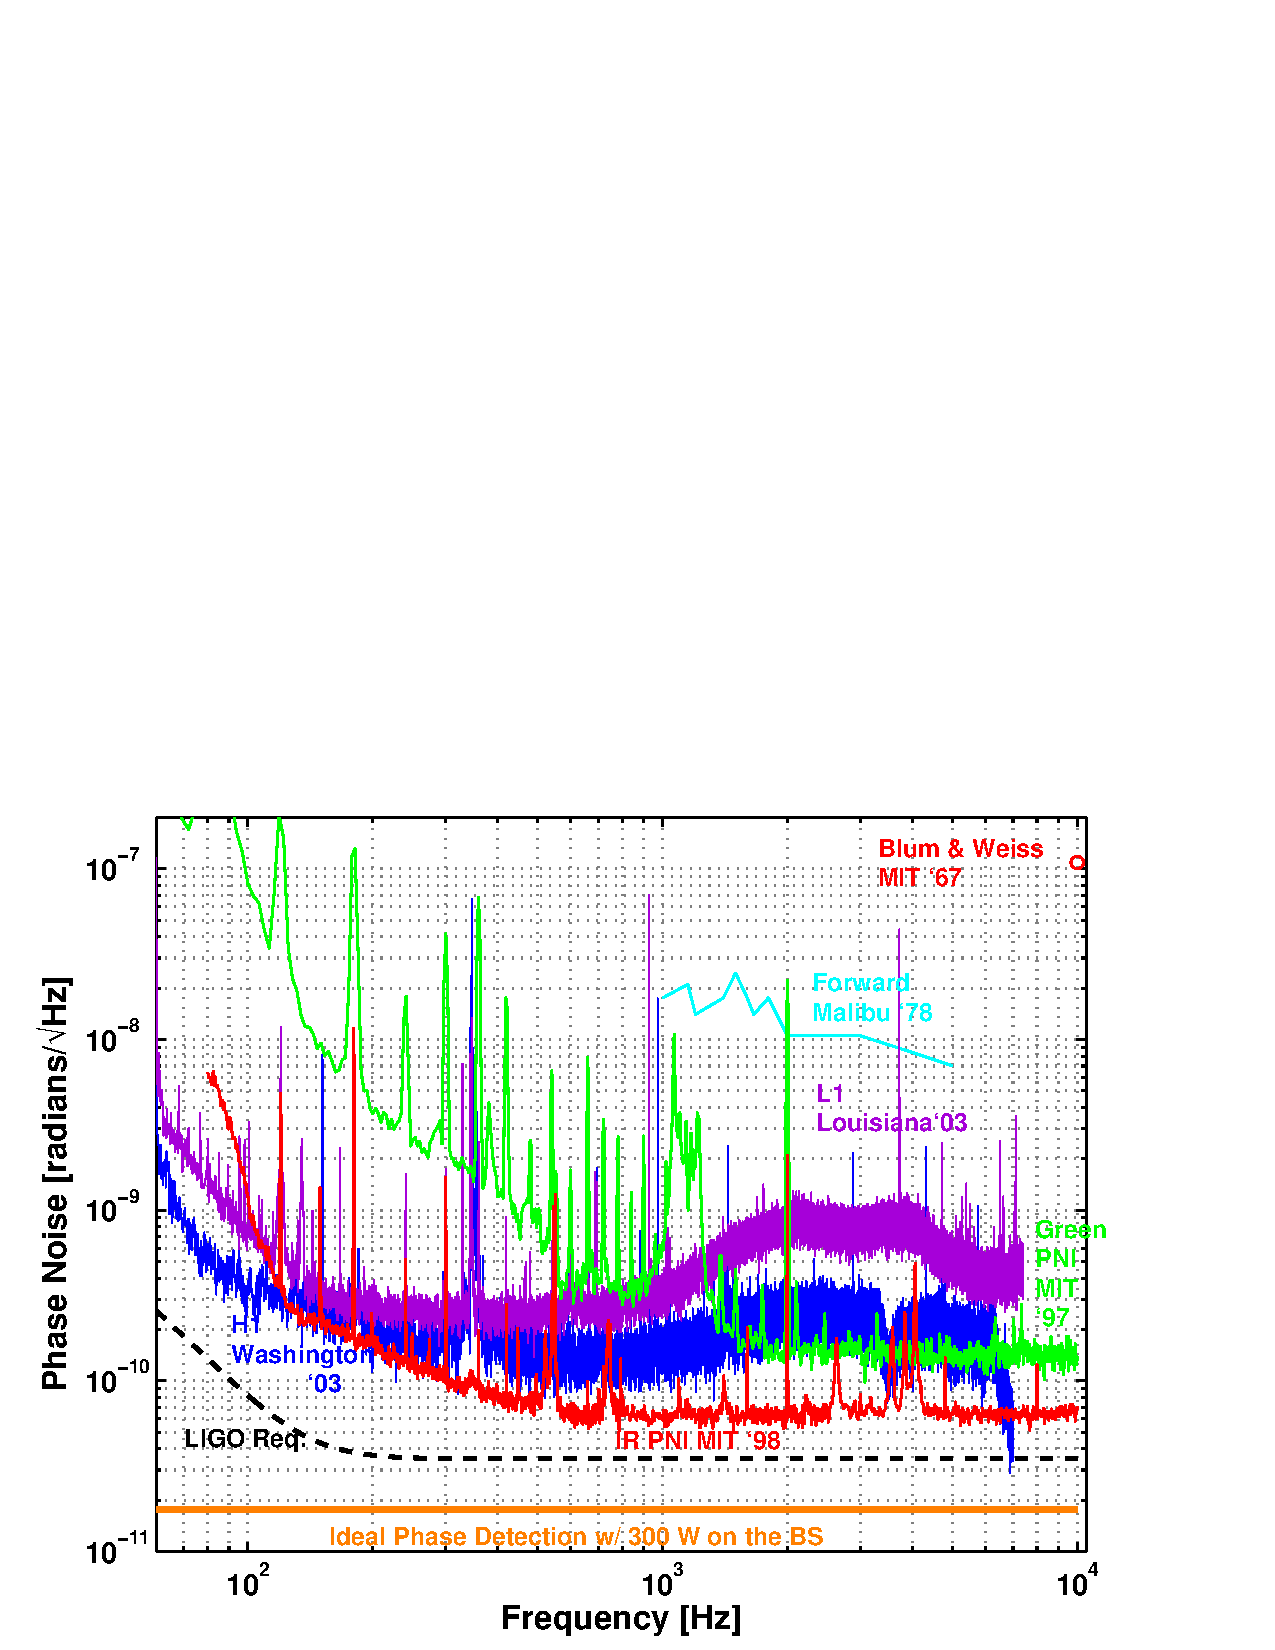
\includegraphics[angle=0,width=6.5in]{Figures/Chap4/PhaseNoises.pdf}}
\caption[Phase Noise]{Evolution of Phase Noise Measurements. The phase shift
         here is defined as the single trip difference between the two arms.
         This convention makes all of the curves a factor of 2 lower than
         in other phase noise comparisons~\cite{Brian:Thesis,Fritschel:PNI}}
\label{fig:PhaseNoise}
\end{figure}



%----------------- CHAPTER 5 -------------------------------------------
%--- SERVOS, SERVOS, SERVOS        -------------------------------------
%% Describes the major servo controls and why they are the way they are.
%% 
%% 
%% 
\chapter{The Control Systems}
\label{chap:controls}

\begin{figure}[!h]
\centerline{\includegraphics[angle=0,width=6.5in]{Figures/Chap5/L1LSC.pdf}}
\label{fig:LSCscreen}
\end{figure}
\clearpage

This chapter describes the major feedback control systems used to keep
the interferometer operating at a point of high sensitivity, and
motivations for the requirements on the control loops and their performance
as of 2003.

Most of the assertions made about the signal readout and the noise couplings
in Chapters~\ref{chap:signals}  and \ref{chap:noise}, respectively, are only 
valid at a very specific operating point: the point at which 
the light is resonant in all parts of the interferometer.

Firstly, resonance means that the round trip phase shift in a single cavity is 
an integer multiple of $2 \pi$. This is to ensure that there is constructive
interference and therefore resonant buildup of the field in the cavity.
In the one-dimensional picture where only the distance between the mirrors
may be adjusted, this is a clear definition.

Secondly, the beam must spatially overlap the same region on each pass. If
the cavity mirrors are overly misaligned the beam will simply miss the
mirrors and fall out of the cavity. Between this gross level and perfect
alignment, there will be some reduction in the power buildup. There will
also be some increased noise couplings~\cite{Yaron:Alignment}.

Finally, the beam's wavefront must remain unchanged on each round trip. This
sets some constraint on the shape of the cavity mirrors. In fact, all of
these criteria are just specific examples of a more general criterion which
states that if the electric field is represented in a basis of
orthogonal modes, the
case of perfect resonance is one in which there is no mode mixing on any
round trip of the cavity. This is further described in Appendix~\ref{app:modes}.

The job of the control systems is to keep the light resonating in the
interferometer. Secondarily, the control systems keep the interferometer's
lengths and angles as close as possible to the perfect resonance condition
in order to prevent degradation of the strain sensitivity.

At last count, there were 107 custom tailored, control loops running the 
interferometer; this does not include any of the systems associated with the 
building HVAC controls, the vacuum system, or the several PID type servos
running inside of some of the commercial instruments. At the time of this
writing there are no servos in operation to actively control the mirrors'
curvature. 

This chapter will focus on the active control of the length 
degrees of freedom of the interferometer, with only a brief description of
the angular controls.


\section{The Length Control Loops}
\label{sec:LSC}

The most recent descriptions of the interferometer's length controls are given
in \cite{Sigg:Readout} and \cite{S1:Inst}. The following paragraph gives a
brief description of the generalities. The rest of the chapter goes into more
detail by first motivating the need for control loops and setting requirements
for them. Then constraints are placed on the loops in the gravitational wave band to reduce
noise pollution from the auxiliary loops.

The average arm length is used in the overall frequency stabilization
scheme and is discussed separately in Section~\ref{sec:CMservo}.

There are several common elements among the 4 control loops:

\begin{itemize}
\item An RF photodetector is used to detect the AM modulated light
      exiting from one of the 3 detection ports. The RF signal is
      demodulated at the resonant sideband frequency ($f_{m}$).
      Both the in-phase and the quadrature-phase components of the
      demodulation are acquired by a 16 kHz ADC after a few stages
      of signal conditioning.

\item The signals are all sent to a VME or rackmount CPU, running custom
      written digital signal processing (DSP) code. The code performs
      many functions including: digital filtering, signal summation,
      triggering, and also provides the signals to the  data 
      acquisition system.

\item After some filtering, the digital signals are passed on to
      a separate set of processors which are set up to handle
      all functions of a specific suspended optic. There are
      typically 1 or 2 optics controlled per CPU.

\item These suspension processors then send the final output signals
      for each optic to a digital-to-analog converter (DAC). The
      DAC signals then go through a set of signal conditioning
      circuits. Finally, there is a power amplifier stage for each
      coil of every suspended optic.

\item The coil currents induce forces on the optic through the magnets
      glued onto them. The interferometer lengths and angles are 
      adjusted by moving the suspended optics.
      
\end{itemize}

\begin{figure}[!h]
\centerline{\includegraphics[angle=0,width=6.5in]{Figures/Chap5/LSC.png}}
\caption[LSC Block Diagram]{Block diagram of the Length Sensing and Control
                            system.}
\label{fig:LSCblock}
\end{figure}


\subsection{Allowed Residual Deviations}
\label{sec:residual_req}

The interferometer is said to be 'locked' when the light is resonating
and the error signals of the control loops are still within their linear
region. To determine how tightly the servos must hold the lock one must
look at the stricter constraint of the apparent strain noise
induced by the deviation from perfect resonance.

So for the length degrees of freedoms a requirement is set on either
$\delta L(f)$, the residual error point spectrum or on 
$\delta L_{\mbox {\tiny RMS}}$,
the total RMS deviation.

\subsubsection{Differential Arm Length ($\delta L_-$)}

As shown in Chapter~\ref{chap:noise}, there are a few noise terms which 
scale linearly with $\delta L_-$. Both the laser amplitude noise and the 
oscillator amplitude noise are really the same physical noise mechanism; 
they modulate the gain of the gravity wave readout channel. 
Seen in that light, the requirement is really on the allowed dynamic 
range of the readout signal. Given that the displacement noise goal is 
$1 \times 10^{-19} \, \mbox{m}/\sqrt{\mbox{Hz}}$
at 150 Hz, the requirement must be that the product of the low frequency
error signal and the gain modulation not exceed this level.

Since the noise term is linearly dependent on two variables, the noise
can be decreased by lowering either component. In practice, attempts
were made to suppress both terms. Further iteration was determined by the
success (or lack of it) in these attempts at suppression.

As a rough estimate, we set the requirement for the residual differential
arm length fluctuations to be that 
{\mathversion{bold} $\delta L_- < 1 \times 10^{-13} \, \mbox{m}_{\mbox {\tiny RMS}}$}.
This sets the requirement on the absolute gain modulation to be such that
$\delta G < 10^{-7}$ for $f = 10-10000  \mbox{Hz}$. 
This ensures that the bilinear noise introduced by laser amplitude noise does 
not exceed 1/10 the displacement sensitivity goal. 


\subsubsection{Differential Recycling Cavity Length ($\delta l_-$)}
Excess noise in the sensing of this degree of freedom couples into the
AS port through the $l_{-}$ control loop. The coupling is determined by
Equation~\ref{eq:mich2darm} . Amplitude noise shows up in this loop the same as
for the $L_{-}$ loop. We would like the amplitude noise term
to not exceed the shot limited sensitivity at this port.

From the shot noise formula for MICH in Appendix I, we have that the
shot noise limited sensitivity is 
$1 \times 10^{-16} \, \mbox{m}/\sqrt{\mbox{Hz}}$.
Using the requirement for the gain modulation, we have a requirement
on the residual differential recycling cavity length that
{\mathversion{bold} $\delta l_{-} < 1 \times 10^{-9} \, \mbox{m}_{\mbox {\tiny RMS}}$}.


\subsubsection{Common Arm Length ($\delta L_+$)}

In order to retain the high power buildup in the interferometer, the
coupled cavity formed by the recycling mirror and the arms must stay
quite close to resonance. The field in the recycling cavity, just
past the recycling mirror is
\begin{equation}
E_{RC} = \frac{t_{RM}}{1 + r_{RM} r_{c}} E_{in}
\end{equation}
A small change in the average arm length changes $r_{c}$, the arm
reflectivity, mostly in phase. This moves the carrier off resonance
in the recycling cavity, reducing the overall buildup.

In the limit of perfect contrast, the shot noise at the AS
port is entirely dominated by the sideband power. Then the reduction
in signal-to-noise is proportional to $\sqrt{P_{\mbox{\tiny BS}}}$, the
power on the Beamsplitter, and for
a 1\% reduction in signal-to-noise we can allow a 2\% power reduction.

This sets a limit of 
{\mathversion{bold} $\delta L_{+} < 2 \times 10^{-12} \, \mbox{m}_{\mbox {\tiny RMS}}$}.


\subsubsection{Common Recycling Cavity Length ($\delta l_+$)}

Using the same reasoning as above, the answer for the recycling cavity
common mode length is that 
{\mathversion{bold} $\delta l_{+} < 2.5 \times 10^{-10} \, \mbox{m}_{\mbox {\tiny RMS}}$}.
Here the main difference is that a change in the recycling cavity
length affects the phase of the carrier field in the recycling cavity
directly and does not get the phase gain associated with the arm. In
fact, the ratio between the requirements for the 2 lengths is just the
phase gain factor for the arm, $r_c'$ ($\approx$ 140).

The recycling cavity Finesse for the sidebands is much less than that
for the carrier and as such, the reduction in recycled sideband power
does not drive this requirement.


\subsubsection{External Disturbances}

Ideally one would like to have an accurate model of the interferometer
which could take as inputs all of the available environmental inputs
and deliver all of the interferometer output signals by including
all of the mechanical, electronic, and optical dynamics from one
end of the interferometer to the other. There is currently a time domain
model under development \cite{e2e:Moriond} with exactly this goal.

Even better, however, is to measure the true length fluctuations
interferometrically. So the design of the length control loops is
bootstrapped. The interferometer was first locked with the simplest
loops that would keep it operating in the linear regime. Then the
loop shapes were iterated until the residual fluctuation requirement
was met.

The disturbance, $\Delta(f)$, to a loop can be expressed in terms 
of a few standard servo parameters:

%\begin{align}
%\delta(f) &= \frac{\Delta(f)}{1+G(f)} & C(f) &= \frac{\Delta(f) G(f)}{1+G(f)}
%\end{align}

\begin{equation}
\delta(f) = \frac{\Delta(f)}{1+G(f)}
\end{equation}

\begin{equation}
C(f) = \frac{\Delta(f) G(f)}{1+G(f)}
\end{equation}

From the above equations, one can see that at frequencies where the
open loop gain, $G(f)$, is high, the control signal, $C(f)$, is nearly
equal to the disturbance. At frequencies where the gain is low, the
error signal, $\delta (f)$, is a more accurate estimator. In practice,
to get the most accurate estimate of the disturbance, either the
control signal or the error signal can be used, but both must be corrected
for the transfer function of the servo loop.

Figure~\ref{fig:dist} shows the disturbance signal for the $L_-$, $l_-$, and $l_+$ loops.

\begin{figure}[!h] 
\centerline{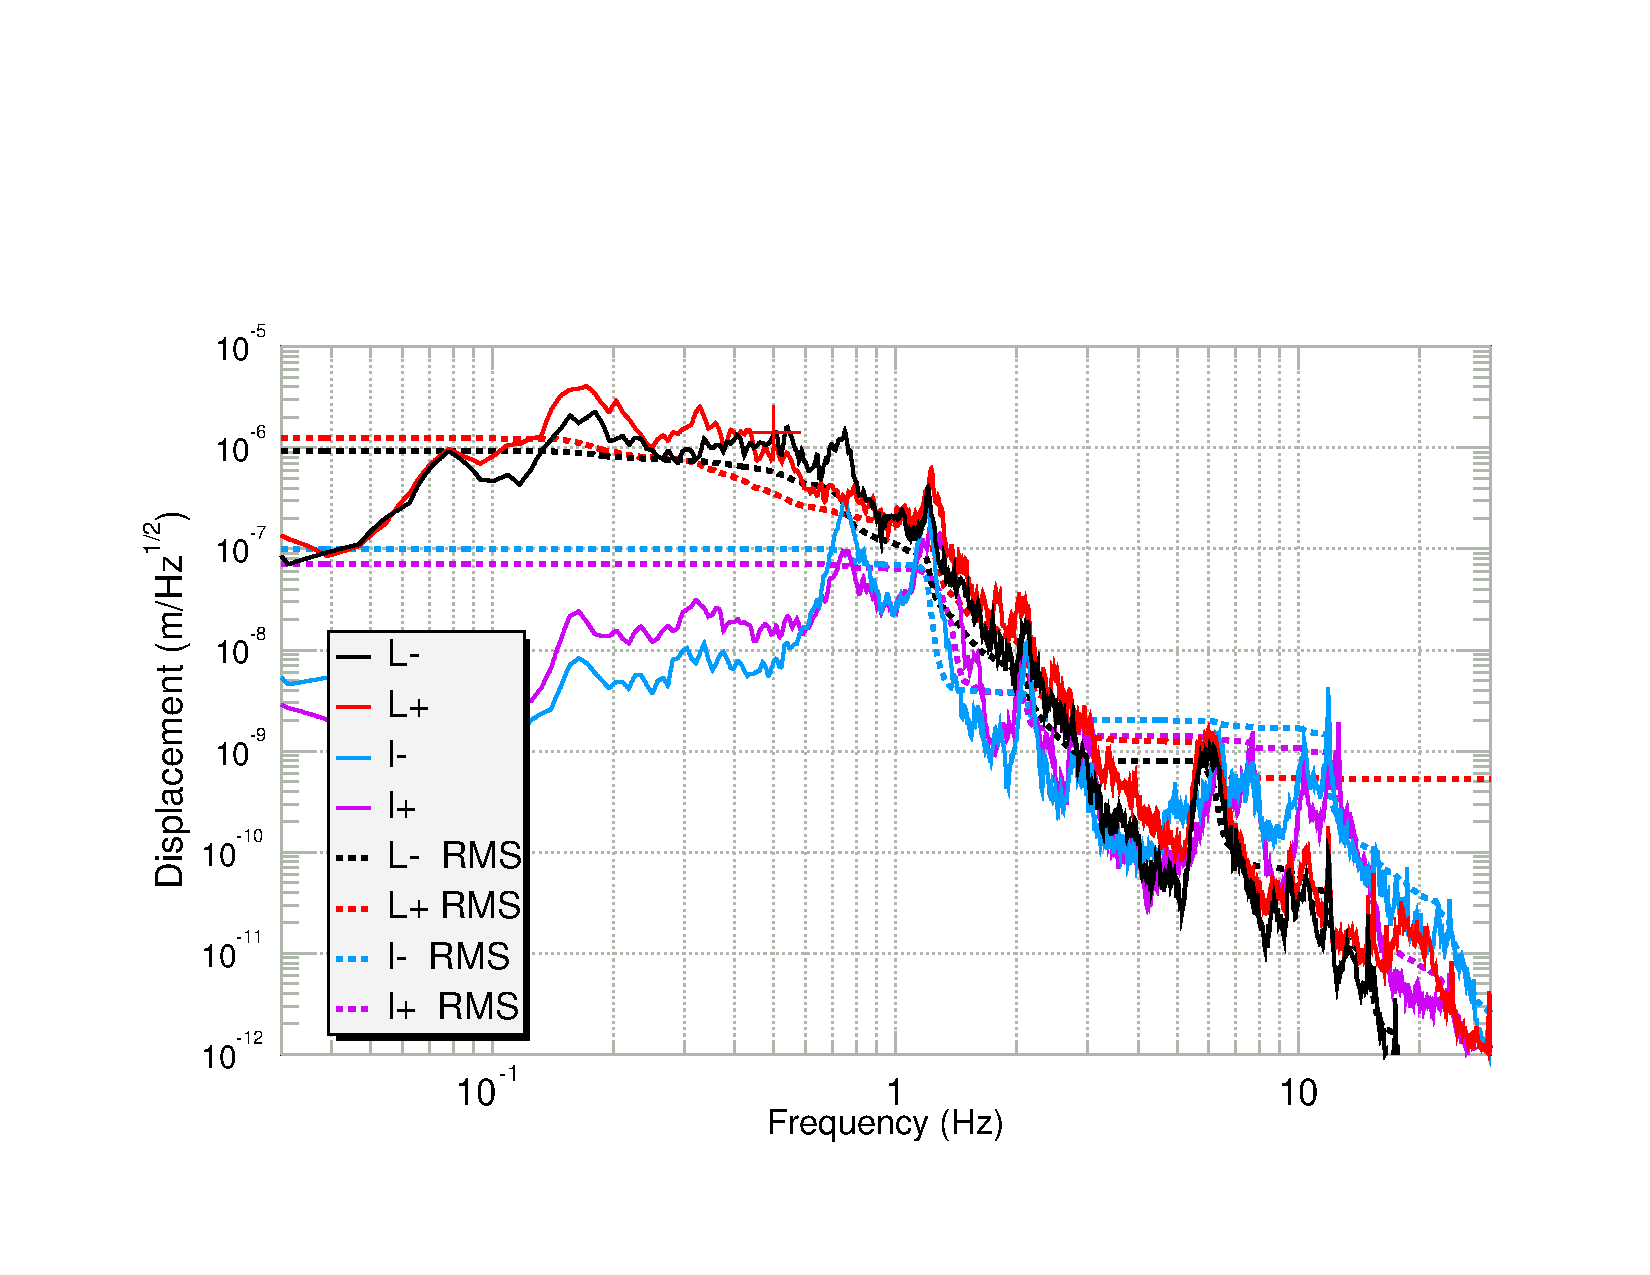
\includegraphics[angle=0,width=6.5in]{Figures/Chap5/disturbances.pdf}}
\caption[Length Disturbances]{Apparent input length disturbance as inferred
         from the servo control signals. The traces labeled 'RMS' show the total
         RMS displacement in the signal in the band,  $f$ - 50 Hz.}
\label{fig:dist}
\end{figure}


\subsubsection{Gain Requirements}

Having the external disturbance spectra and a goal for the residual 
fluctuations allows us to make a first iteration on the control loops. The
fact that the loops are digitally implemented allows one to quickly iterate
on the loop transfer functions and achieve the desired performance.

The Bode plots in Figure~\ref{fig:Loops} show the open loop gain of 
three of the four main length control loops.

\begin{figure}[!h] 
\centerline{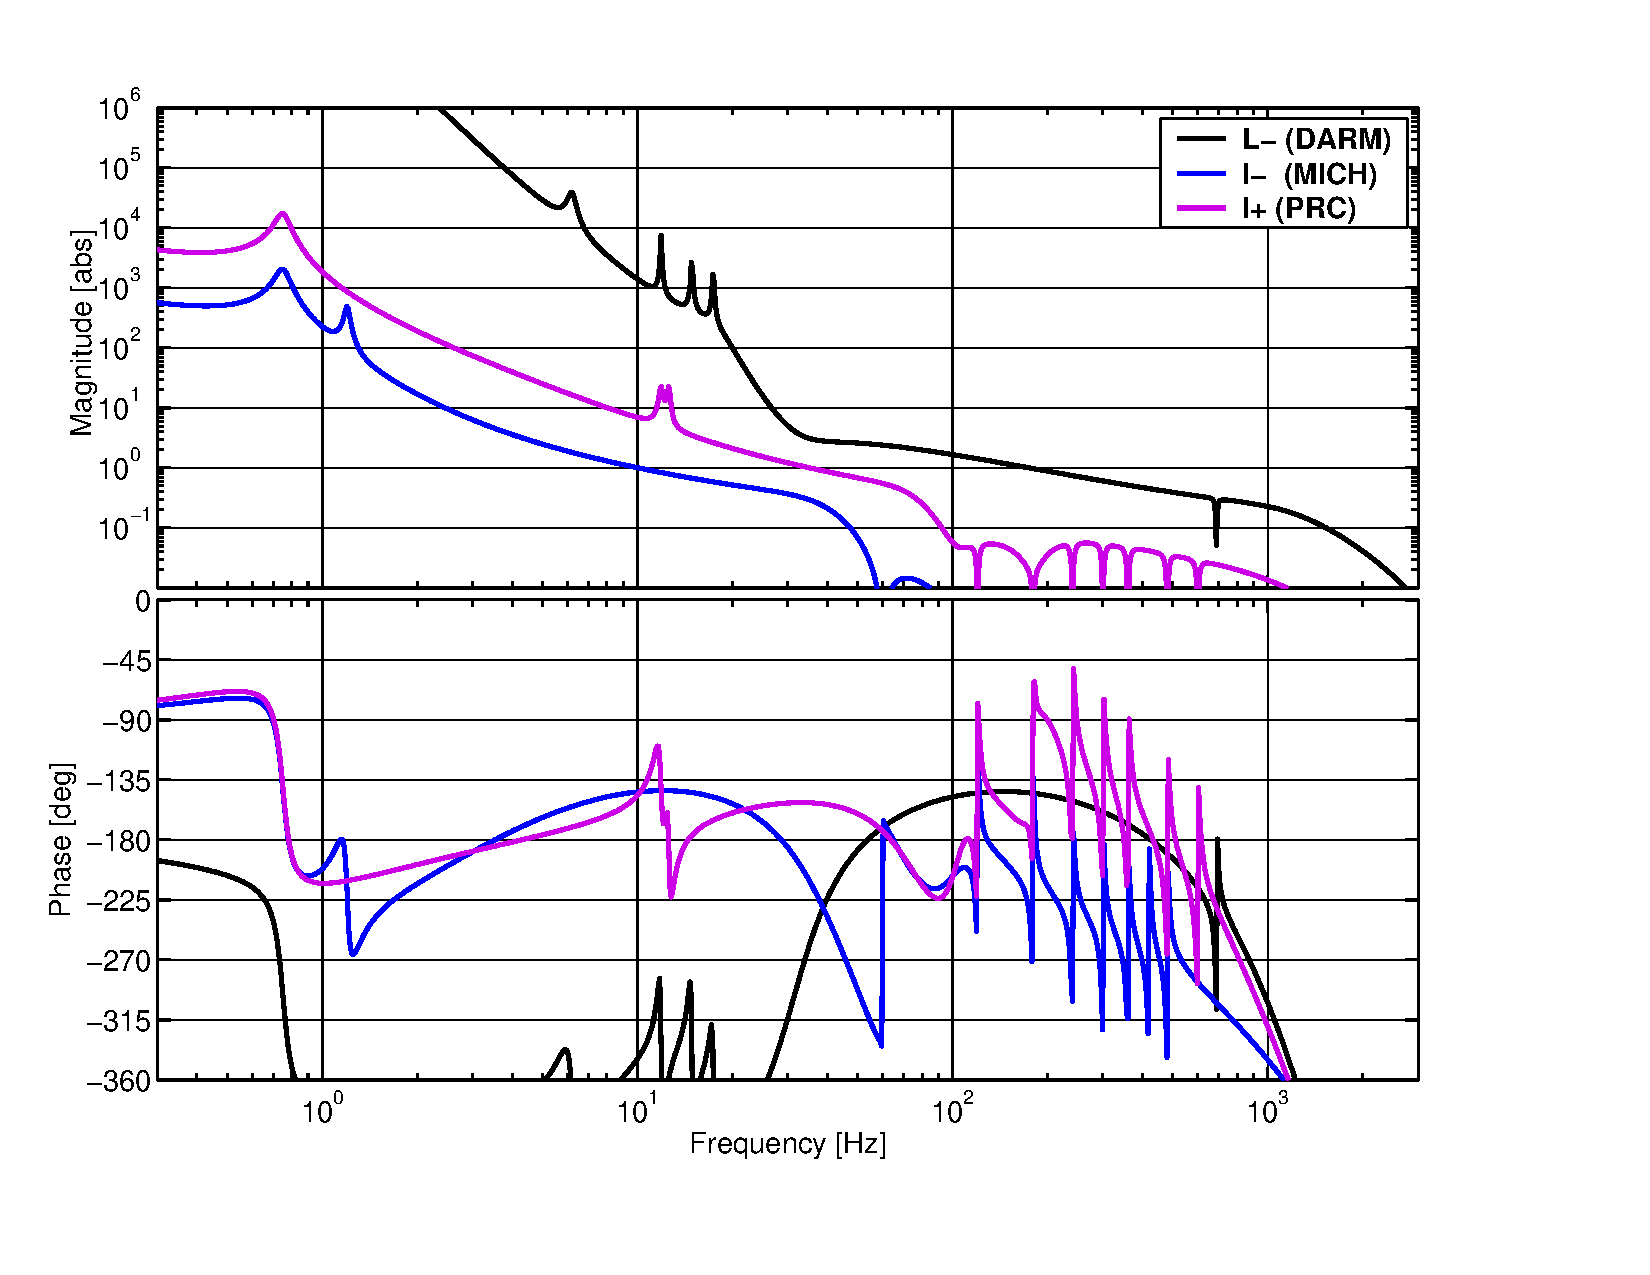
\includegraphics[angle=0,width=6.5in]{Figures/Chap5/LSC-Loops.pdf}}
\caption[Length Loops]{Open loop gain of three length control servos.}
\label{fig:Loops}
\end{figure}
With these loops the measured loop residuals meet the requirement. 
Figure~\ref{fig:residuals} shows the in loop error signals.

\begin{figure}[!h] 
\centerline{\includegraphics[angle=0,width=6.5in]{Figures/Chap5/residuals.png}}
\caption[Residual Fringe Offsets]{Spectra of the servo error points calibrated
         in meters. These are the true length offsets, assuming no significant
         offsets are added in at the error point.}
\label{fig:residuals}
\end{figure}


\subsection{Noise Pollution}

In the gravitational wave band the motion in the auxiliary loops must be controlled to a level
such that induced strain noise spectral density is at the SRD/10 level. The
introduced noise is a function of three parameters of the auxiliary loop:
the sensing noise, the loop gain, and the coupling to AS\_Q. So attempts
were made to reduce all three terms.

\subsubsection{Auxiliary Sensing Noises}

In Figure~\ref{fig:POBnoise}, the noise in the $l_-$ and $l_+$ loops is shown. 
All of the noise above 20 Hz can be seen as some sort of sensing noise in 
that it is not a direct representation of length fluctuations. 

\subsubsection{Gravitational wave band filtering}

Since the $l_{-}$ \& $l_{+}$ signals are full of only sensing noise in
the gravitational wave band one would like to reduce, as much as possible, the contribution
of the control signals to AS\_Q. To do this, aggressive digital stopband
filters were designed to lower the loop gain in the sensitive 60-200 Hz
band.


\subsection{The real loops}

Each of the three main length control loops were individually tailored and
have intricate transfer functions (as shown in Figure~\ref{fig:Loops}).
These following sections list a few of the driving considerations involved
in designing the loops. In all cases, the gain at low frequencies must be
high enough to suppress the noise shown in Figure~\ref{fig:dist} to the
levels specified in Section~\ref{sec:residual_req}. In addition, the servos
must have sufficient gain and phase margin to remain stable in the face
of fluctuating optical gain.


\subsubsection{L$_-$ (a.k.a. DARM)}

The DARM loop controls the differential arm length. The gravitational wave
signal is reconstructed from the error point signal (AS\_Q) of this loop.

This is the highest bandwidth digital servo loop in the interferometer. It
is limited at high frequencies by the phase shifts associated with the
anti-aliasing filters before the ADC and after the DAC (see 
Figure~\ref{fig:DARMmodel}). 

There is also the issue of the high Q ($\sim 10^5$) mechanical
resonance of the suspension wire at the ($\approx$345 Hz) 'violin' frequency;
there is a poorly understood interaction with this resonance which sometimes
requires attenuation through the use of very narrow digital notch filters.
The coupling seems to come and go; the interferometers often run for months
without notches and without any instability.

At even higher frequencies (e.g. 6.6 kHz, 9.3 kHz, and 13 kHz), the servo must have a low 
enough gain to not excite the even higher Q ($10^5 - 10^7$) internal mode 
resonances of the mirrors themselves. These typically have stopbands of 
80-100 dB, widths of a few Hz (to accommodate the temperature dependent 
frequency drift of the modes), and are very near the Nyquist frequency (8192 Hz) 
of the digital system. The modes
with frequencies greater than 8192 Hz are excited through a double aliasing
effect. They are finitely attenuated by the ADC's anti-aliasing filter, but
then still show up in band at 
$f_{aliased} \simeq f_{Nyquist} - (f_{mode} - f_{Nyquist})$. If not filtered
out, this then propagates out through the DAC and is again aliased up to high
frequencies. This completes a loop involving the internal mode which can then
get excited and cause saturation in the sensing electronics. Once a stopband
filter has been tuned for every mode on every driven optic, the modes are
no longer a problem.


\subsubsection{l$_-$ (a.k.a. MICH)}

The MICH loop has a low ($\sim$10 Hz) unity gain frequency. There are two
reasons for this: 

The gain at high frequencies must be kept low to reduce the
the coupling from $l_-$ sensing noise to $L_-$ strain noise. The unity gain
frequency is constrained by the phase lag due to the $\sim$ 50 Hz bandstop filter.

The other constraint is that this loop has a peculiar intermittent coupling to the 
\emph{roll} mode of the recycling mirror. This mode is at $\approx$18 Hz and will
occasionally get excited and grow exponentially if the MICH unity gain
frequency is set to within a few Hz of 18 Hz. It is not understood why this
coupling is unstable.


\subsubsection{l$_+$ (a.k.a. PRC)}

The PRC loop could be run with as high a bandwidth as the DARM loop and has the
same considerations with respect to higher frequency mechanical resonances. The
main constraint on the bandwidth is the noise coupling. So the gain has been
lowered to add aggressive filtering in the 60-200 Hz band. In the long term
the sensing noise in both the $l_+$ and $l_-$ loops will have to be reduced and
the coupling to the anti-symmetric port reduced through the use of off
diagonal length actuation: driving the $L_-$ length by the just the amount
necessary to cancel the measured coupling factor. This technique was
implemented successfully on the Livingston interferometer for the $l_-$ 
servo during the latest Science Run (S3).



\subsection{The Common Mode Servo}
\label{sec:CMservo}
Gravitational radiation can produce both differential and common mode strains
of the arm cavities. We choose to only use the differential mode read out
for gravitational waves because the common mode signal is polluted with a
large level of laser frequency noise.

There is a choice to be made in what to pick as the reference in all of these
length measurements. For the common arm length this amounts to whether the laser
wavelength should be locked to the arms or the arms locked to the laser. Since
we have made such effort to isolate the test masses from external disturbances
the average arm length proves to be a much better reference at audio frequencies
(above 20 Hz).

\begin{figure}[!h]
\centerline{\includegraphics[angle=0,width=6.5in]{Figures/Chap5/FreqNoiseReq.pdf}}
\caption[Laser Frequency Noise]{The spectral density of the free running 
         frequency noise of the MOPA is compared to the SRD/10 requirement 
         based upon an arm cavity reflectivity difference of 0.5\%.}
\label{fig:FreqNoiseReq}
\end{figure}
From Chapter~\ref{chap:noise}, we have the coupling of frequency noise 
into the strain output.
Figure~\ref{fig:FreqNoiseReq} shows that the laser frequency noise must be 
suppressed by a factor of 10$^8$ to bring it to 1/10th of the strain 
sensitivity goal. There is more to
the problem than just gain, however. As the laser is further quieted, each
following reference to which the frequency is servoed must be more quiet than
the last.

To achieve the required suppression, multiple, hierarchical servos are used.
Before the light is injected into the vacuum, the large, raw laser fluctuations 
are actively and passively suppressed (see Section~\ref{sec:PSL}). 
Laser noise above 1 MHz
is filtered out by passing through a medium finesse ring cavity called
the pre-mode cleaner. By locking the laser frequency to a short ($\approx 20 cm$), 
rigid reference cavity with a $\sim$100 kHz servo loop the laser frequency noise
is stabilized by a factor of $\sim$1000.
 
This pre-stabilized light is then locked to a much quieter, suspended,
12 m cavity called the Mode Cleaner, described in Appendix~\ref{app:ModeCleaner}. 
Finally, the light transmitted through the Mode Cleaner is locked to the 
average length of the 4 km arm cavities.

\begin{figure}[!h]
\centerline{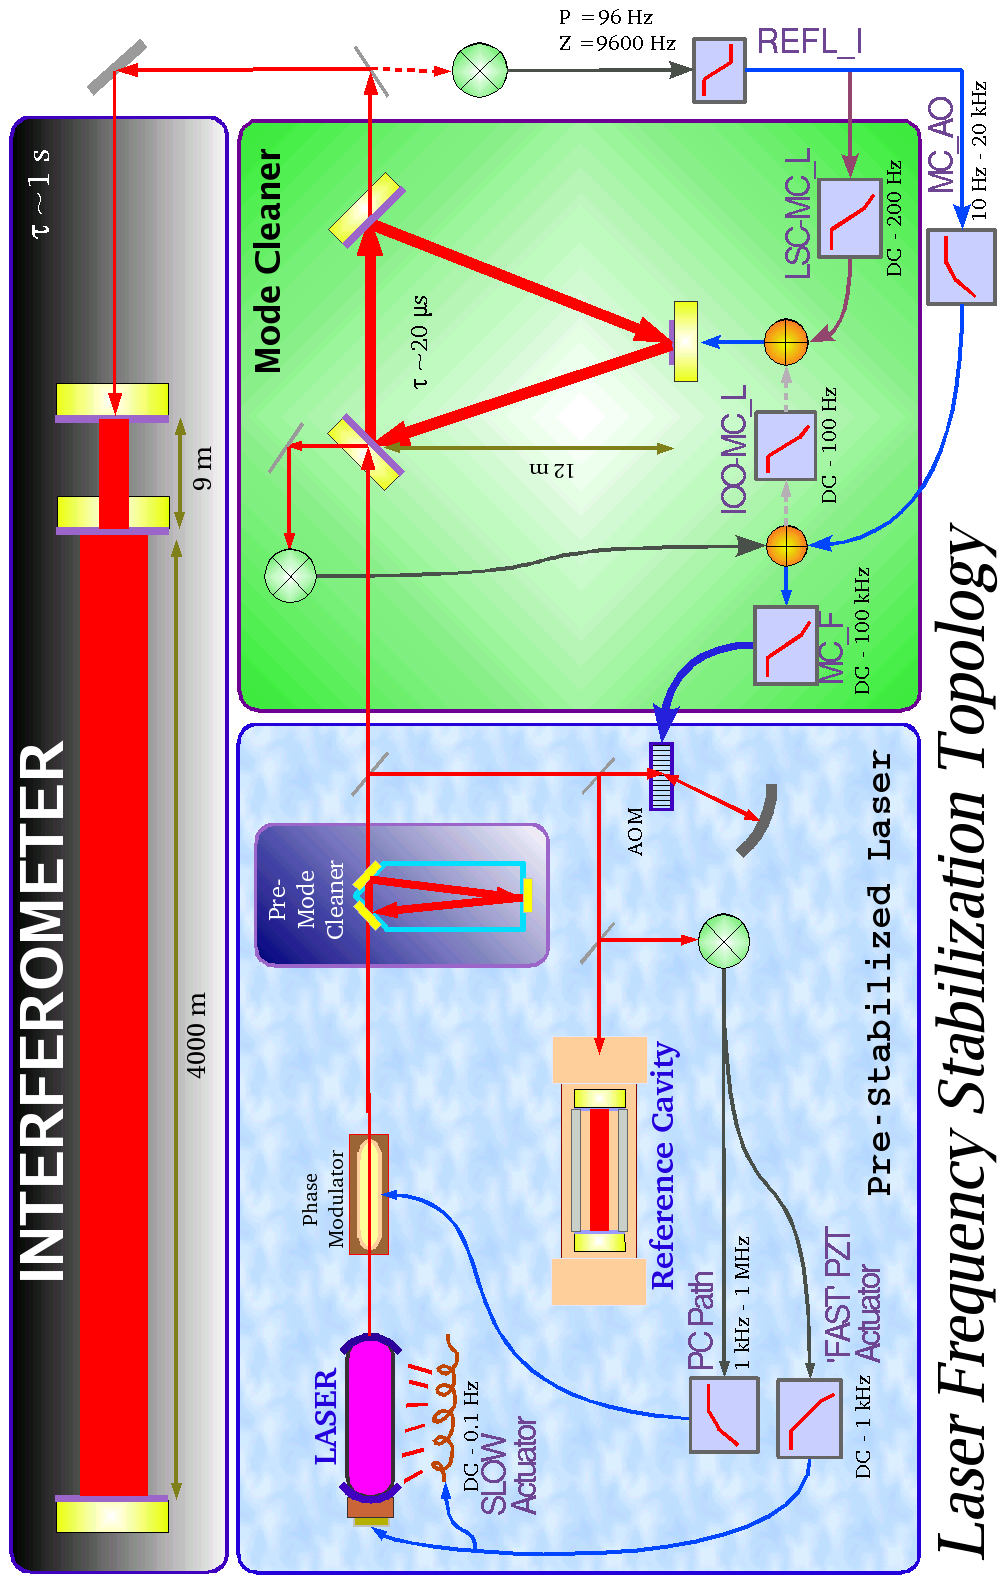
\includegraphics[angle=0,height=7.5in]{Figures/Chap5/CMs90.png}}
\caption[CM Servo Block Diagram]
        {Block diagram of the Global Frequency Stabilization Topology.}
\label{fig:CMblock}
\end{figure}
Ignoring for the moment the internal workings of the mode cleaner and the laser
we can focus on the mechanics of the common mode servo. The difficulty is that
although the laser wavelength is already tightly locked to the mode cleaner
length, it is necessary to adjust the wavelength to match the common mode arm
length and yet keep the light resonating in all the cavities simultaneously.

To see how this is done, it is useful to look at what the MC servo really does.
It derives an error signal which is nominally proportional to the difference
between the round trip length of the cavity and the wavelength of the light
incident on the cavity, modulo an integer number of wavelengths. The common
mode servo works by adjusting the reference to which the laser wavelength
is compared.

At low frequencies, the common mode servo drives the mode cleaner length. This
adjusts the laser frequency since the laser frequency is already locked to the
MC length. Above a few hundred Hz, the length feedback is limited by the
wire resonances of the MC suspension.

A fast, low dynamic-range path, called the additive offset (AO), is used up to 20 kHz.
The AO path works by adding electronic offsets into the MC error
point. The MC servo shifts the laser frequency in order to cancel this offset,
but the resulting laser frequency offset serves the purpose of the AO. 
This might pose a problem, since by introducing an offset in the MC
error point, the laser is being pulled off of resonance in the MC. However,
the actual AO control signal is quite small; only a few Hz peak-peak, as 
compared to the $\sim$8 kHz linewidth of the MC resonance.


\begin{figure}[!h]
\centerline{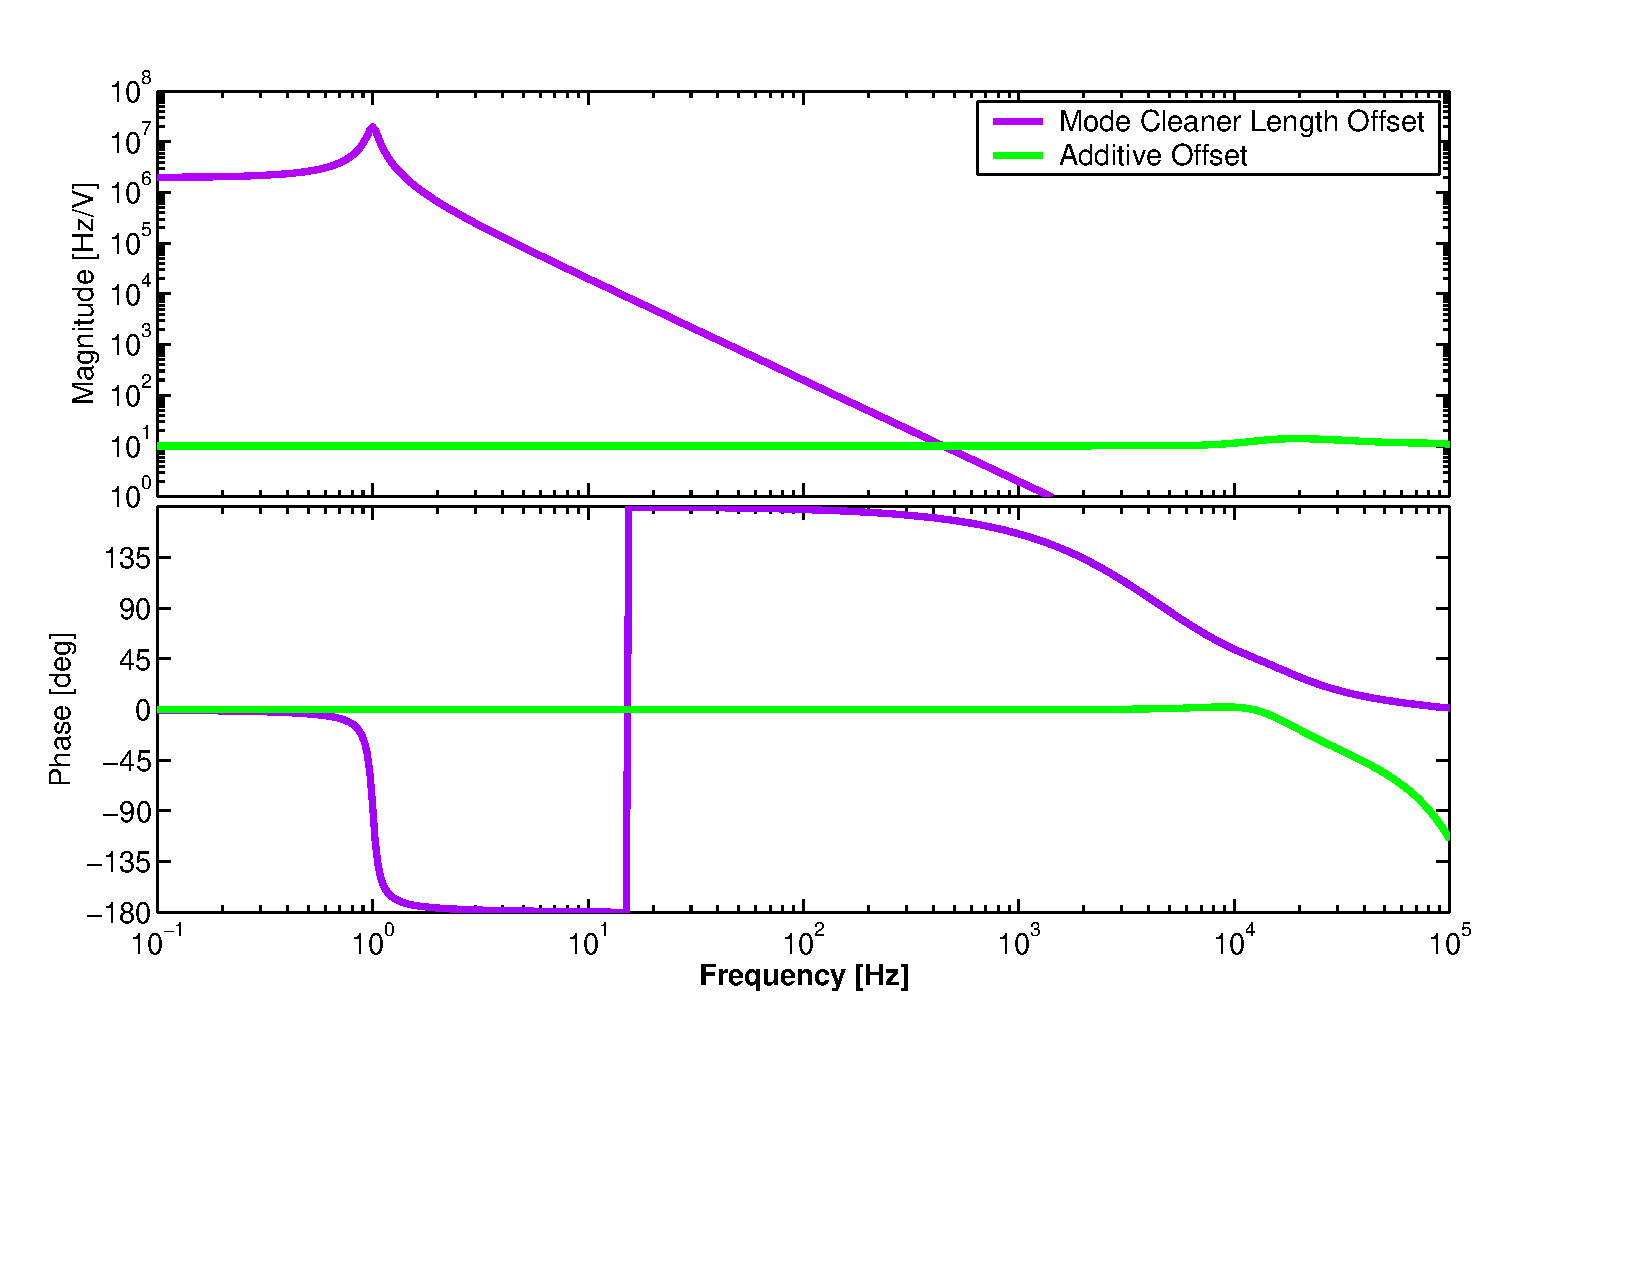
\includegraphics[angle=0,width=6.5in]{Figures/Chap5/cm_acts.pdf}}
\caption[CM Actuators]{Shown are the frequency responses of the two actuators
                       used in the common mode servo. The response is to voltage
                       applied at the coil driver (MCL) and the MC servo mixer
                       (AO).}
\label{fig:CMactuators}
\end{figure}


Figure~\ref{fig:CMactuators} shows the frequency response of the two CM servo
paths. At high frequencies, very large voltages would be required to get
sufficient actuation authority in the MC length path and so the two paths
are crossed over as shown in Figure~\ref{fig:CMbode}. The AO bandwidth is
limited at high frequencies by the finite bandwidth of the MC servo.


\begin{figure}[!h]
\centerline{\includegraphics[angle=0,width=6.5in]{Figures/Chap5/CM-Loops.png}}
\caption[CM Loops]{Open Loop Gain of the total Common Mode Servo and of the
                   individual MCL and AO paths.}
\label{fig:CMbode}
\end{figure}


Figure~\ref{fig:CMcontrols} shows the control signals of the CM servo. In the
regime where the loop gain is high the control signal can be used to estimate
the input disturbance - the frequency noise on the light transmitted by the
MC.


\begin{figure}[!h]
\centerline{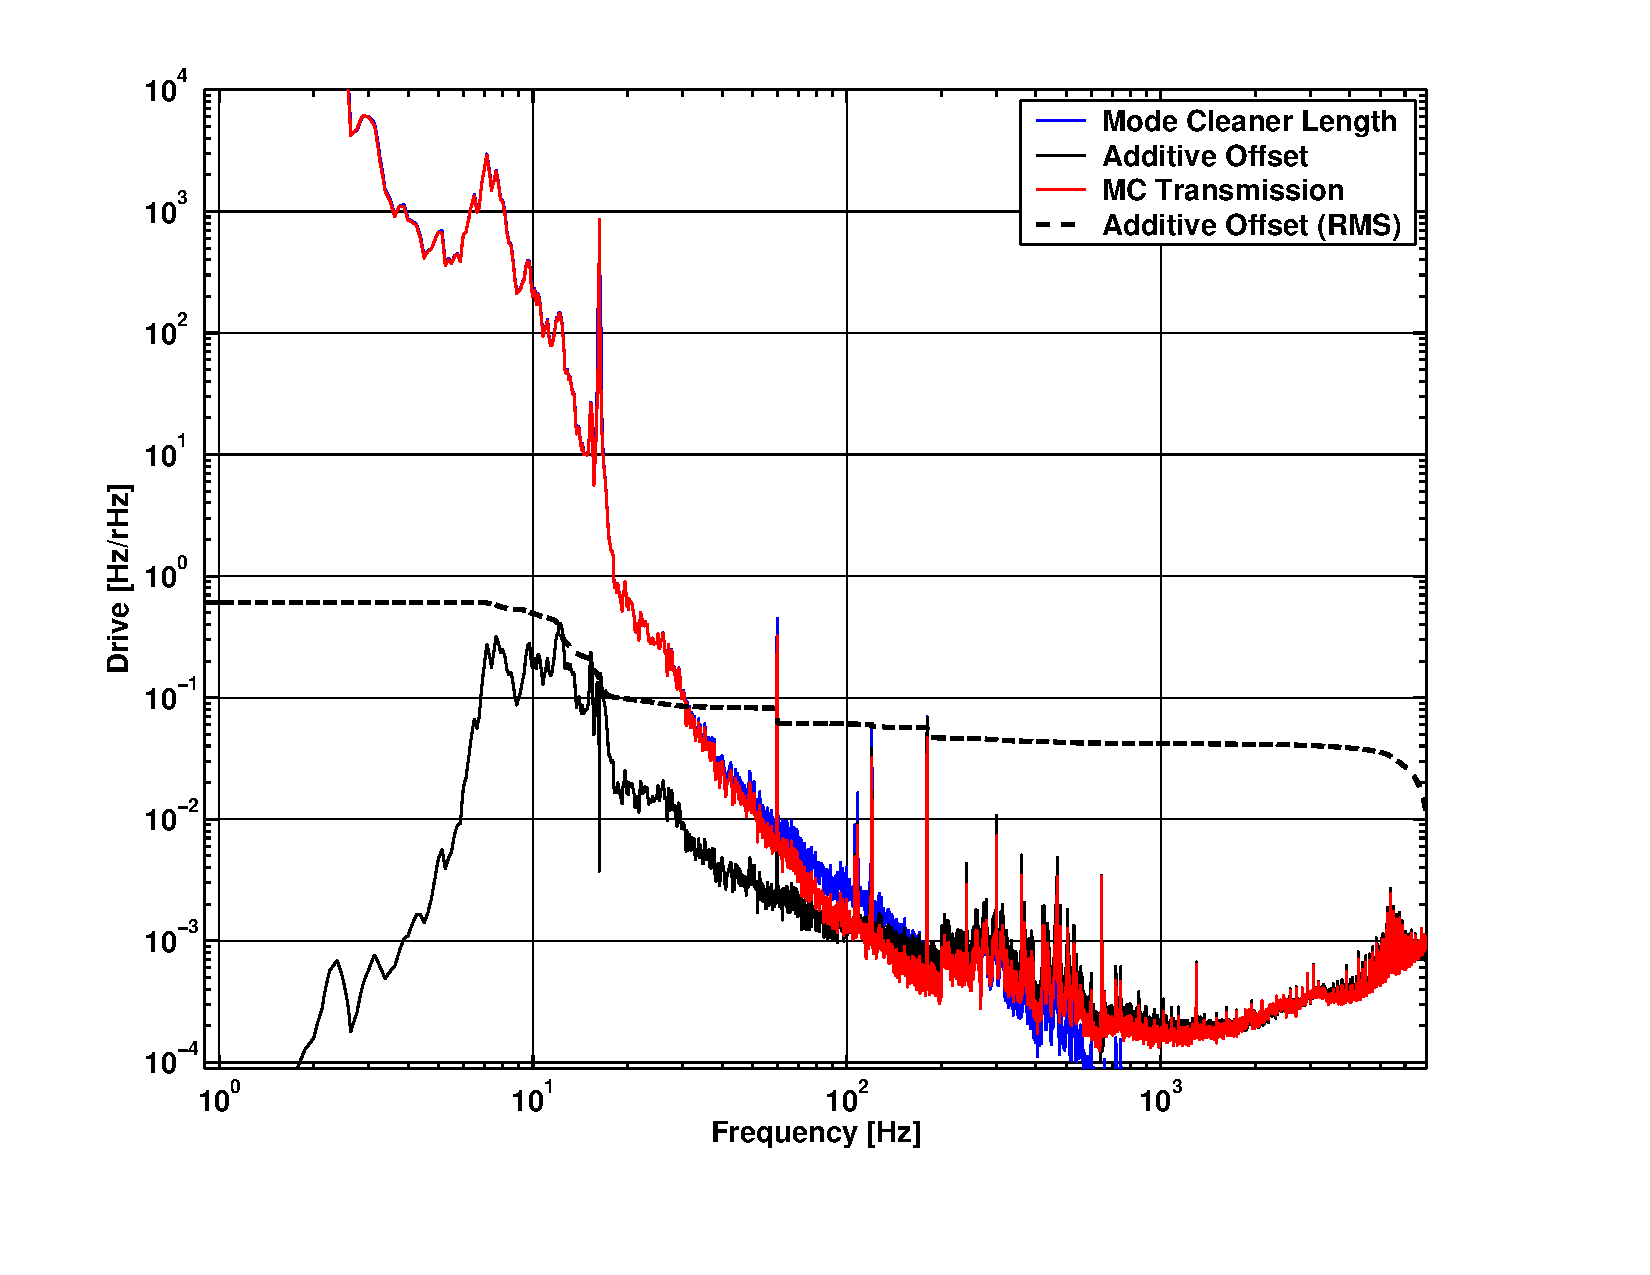
\includegraphics[angle=0,width=6.5in]{Figures/Chap5/cmnoise3.pdf}}
\caption[CM Noise]{The MCL and AO control signals are shown. Also shown is the
         total frequency noise transmitted by the MC, calculated from the CM
         control signals. Also shows is the integrated RMS of the AO control.}
\label{fig:CMcontrols}
\end{figure}


Finally, the ultimate performance of the entire frequency stabilization scheme
can be summed up by Figure~\ref{fig:CMnoise}. The plotted requirement is the
level of frequency noise which will equal 1/10 of the strain sensitivity goal.

This curve is calculated using the frequency domain interferometer model which
uses as inputs the measured frequency noise to differential strain coupling. This
curve along with the measured CM servo loop gain establishes a requirement on the
frequency fluctuations on the light leaving the mode cleaner. This requirement is
compared to the measured performance of the mode cleaner in 
Appendix~\ref{app:ModeCleaner}.

\begin{figure}[!h]
\centerline{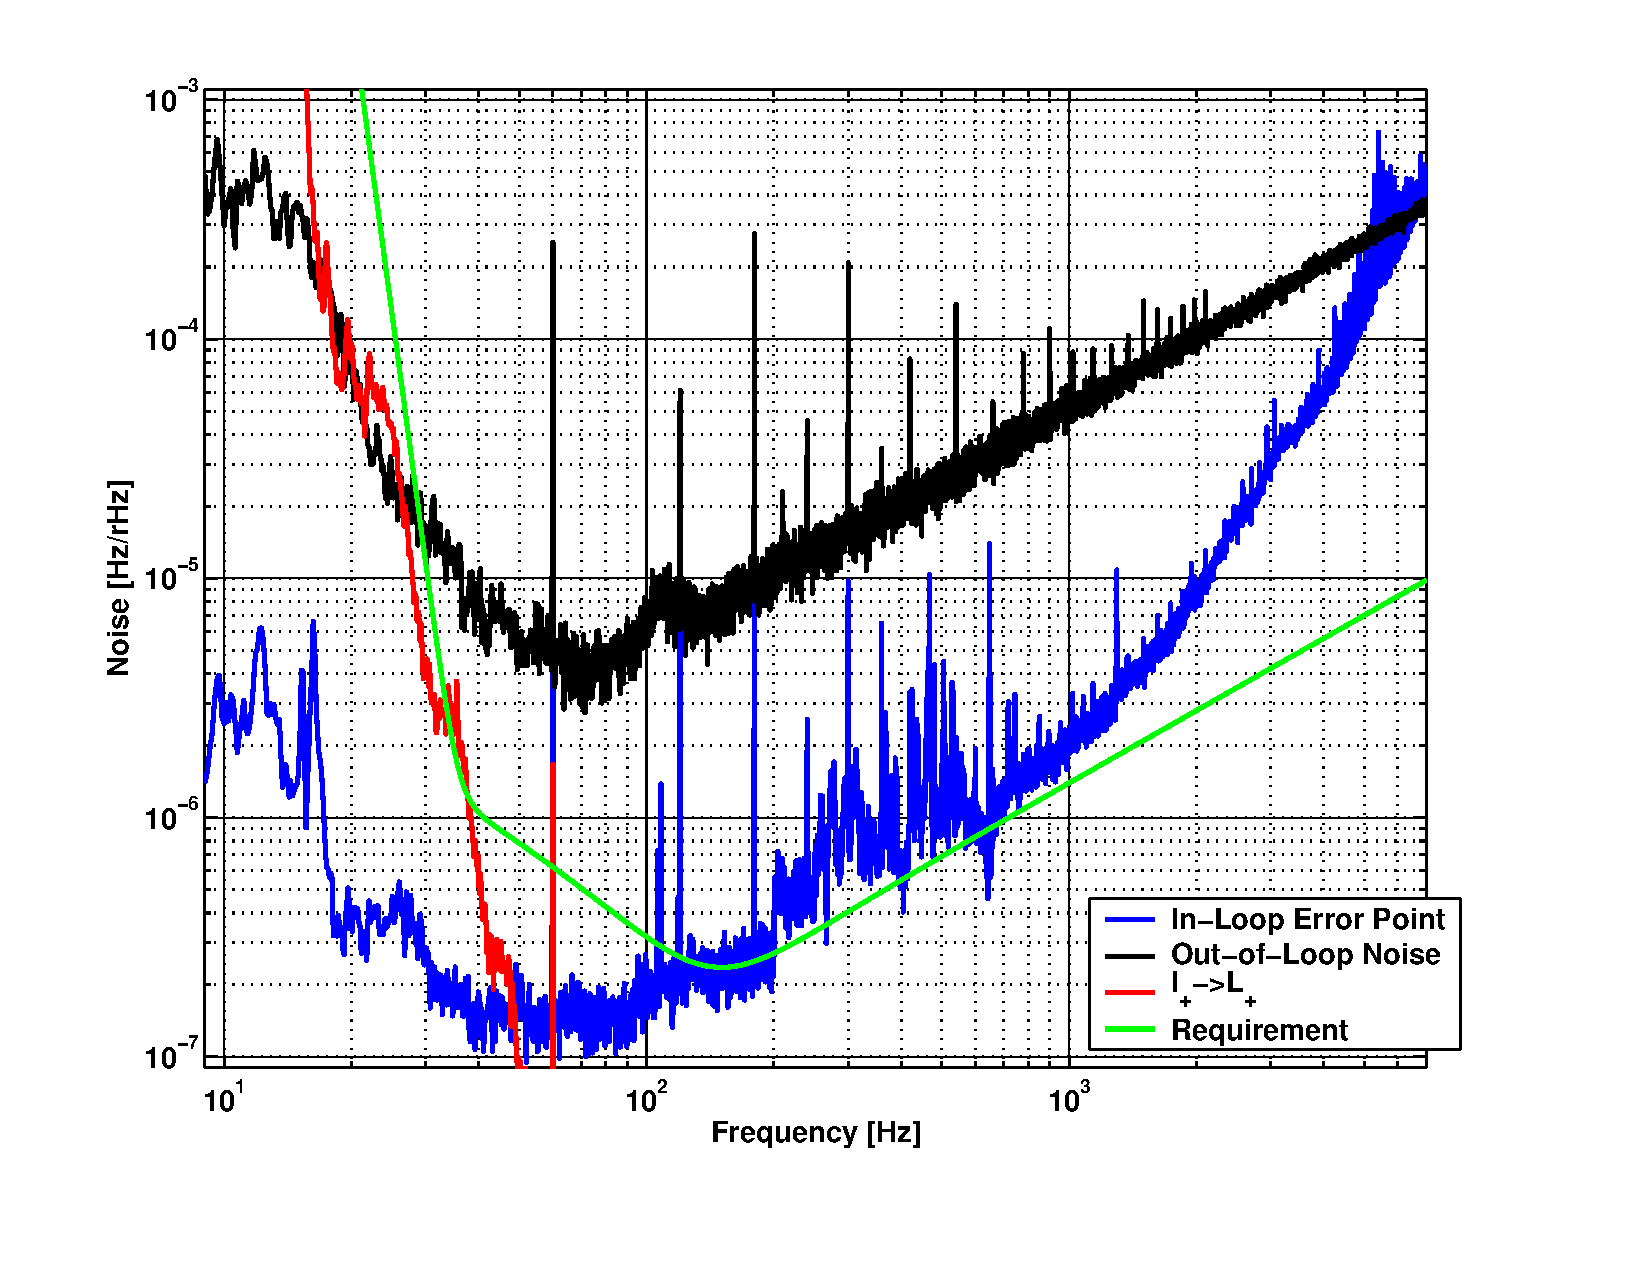
\includegraphics[angle=0,width=6.5in]{Figures/Chap5/cmnoise3b.pdf}}
\caption[Residual Frequency Noise]{The in-loop error point is compared to the
           sensing noise floor to show that the in-loop error point 
           underestimates the true noise. The plotted requirement is SRD/10.}
\label{fig:CMnoise}
\end{figure}

\subsubsection{Parasitic Interferometers}
\label{sec:CMscatter}

On the laser table, vibrations of the optical mounts put phase noise on the light
which then is measured in the mode cleaner control signal. This frequency noise
has been reduced somewhat through the use of stiffer mounts and acoustic isolation
of the table. The mode cleaner servo gain is sufficient to make acoustics from the
laser table an insignificant contributor to the interferometer noise.

Acoustic coupling on the mode cleaner's output optical table dominates the
frequency noise on the light incident on the interferometer in the 100-1000 Hz
band. This still needs to be reduced by $\sim$10.

The acoustic noise on the mode cleaner table is injected at the error point
of the servo as sensing noise. It is only characterized because we then measure the
mode cleaner noise performance with an even quieter reference in the common mode
servo. For the common mode servo, there is no further check and so the acoustic
noise coupling there is sent unsuppressed into the interferometer and is
probably more severe.

The steep rise below 100 Hz in the 'out-of-loop' trace of Figure~\ref{fig:CMnoise} is due
to a parasitic scattering path somewhere in the path between the recycling
mirror and the readout PD for the interferometer's reflected port.


\section{Angular Controls}
\label{sec:ASC}

The Angular Sensing and Control system is still being commissioned and
refined. This section briefly mentions the different angular sensing
schemes which are used. 


There are three chief feedback paths for the angular degrees of freedom
of the interferometer:

\begin{itemize}

\item The first, primitive stabilization is done by damping the pitch
      and yaw eigenmodes of the suspended optics using the local 
      sensors~\ref{sec:OSEMs}. These provide some stability at the
      pendulum frequencies, but is limited by the large motions of the
      isolation stack to which the suspension cage is mounted. The high
      frequency angular sensing noise of the local sensors is
      $\approx10^{-10} \, \mbox{radians}/\sqrt{\mbox{Hz}}$. This requires
      a very low bandwidth servo ($\approx 2$ Hz) with aggressive low
      pass filtering.

\item The second level of angular stabilization comes from optical levers.
      Each optical lever is a fiber coupled diode laser and a
      quadrant photodetector, each mounted to a steel pier outside
      of the vacuum. From $\approx$0.3-5 Hz, these are better angular
      references than the local sensors. Their chief benefit is in simplicity:
      these servos work independent of the locked state of the interferometer.
      The noise in this sensor is somewhat better than the local sensors,
      $\approx10^{-11} \, \mbox{radians}/\sqrt{\mbox{Hz}}$, in a broadband
      sense but is dominated by acoustic/mechanical resonances which
      are 10-50X larger.

\item The ultimate solution to angular sensing is the Wavefront Sensor (WFS)
      system~\cite{Yaron:Alignment,Alignment:Applied,Nergis:Thesis}. These are 
      RF quadrant detectors working
      on a heterodyne readout system similar to that used in the length
      sensing. The WFSs sense relative tilts and translations between the carrier
      and RF sideband fields by taking differences between the demodulated outputs
      of the quadrants. The shot noise limited sensing noise of these sensors
      is, in principle, far superior to the other sensors. The broadband
      noise floor varies from $10^{-13} - 10^{-14} \, \mbox{radians}/\sqrt{\mbox{Hz}}$,
      depending on which sensor.

\item A non-RF part of the WFS scheme is the DC quadrant photodetectors 
      monitoring the weak beams transmitted through the arm cavity end 
      mirrors. These fix the beam position onto the center of the end mirrors.
      The angular sensitivity of these sensors is comparable to the WFS, but
      they have the disadvantage of being fixed to the local reference frame
      of the ground at the end stations.

\end{itemize}


\begin{figure}[!h]
\centerline{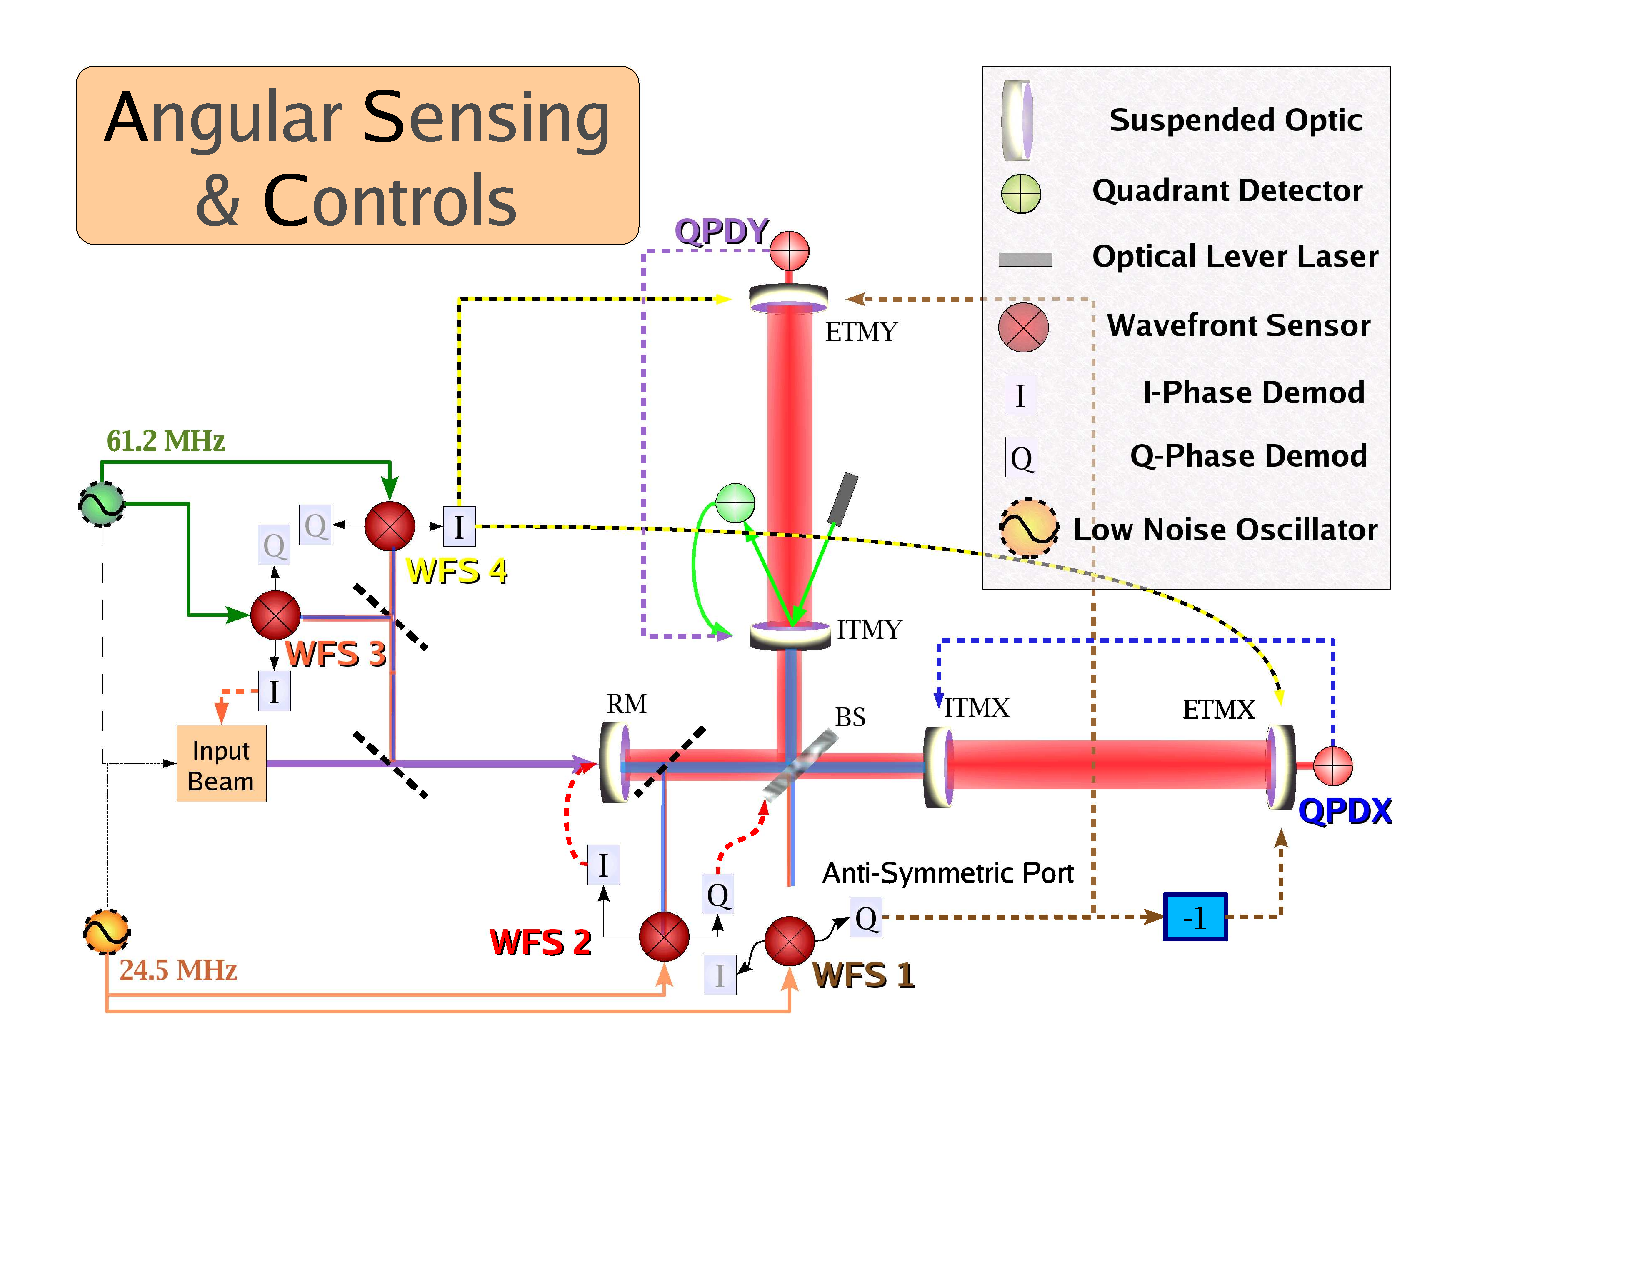
\includegraphics[angle=0,width=6.5in]{Figures/Chap5/ASC2.pdf}}
\caption[ASC Block Diagram]{Block diagram of the Angular Sensing and Control
                            system. Only one optical lever setup is shown for
                            simplicity, although there is one per optic.}
\label{fig:ASCblock}
\end{figure}

Figure~\ref{fig:ASCblock} shows a rough outline of the sensing and feedback
topology. Each of the suspended large optics has an optical lever servo. The
feedback diagram is a simplified version of the real feedback topology which
uses multiple mirrors in the feedback for each WFS. This arrows in this diagram
are only to indicate the principle degree of freedom of the feedback. 

During the S2 run, the Livingston interferometer had only WFS1 running,
with feedback set to drive the differential ETM angle. This is the most
critical angle in the interferometer; without control of this degree of
freedom, the power at the Anti-Symmetric port varies wildly, making many
servos unstable. The Hanford 4 km interferometer had nearly all of the 
WFS loops closed with a low bandwidth and for the S3 run managed to close all
WFS loops. 

\section{Local Damping}
\label{sec:OSEMs}

The wire suspension (see Section \ref{sec:SUS}) for the interferometer's central mirrors
is soft in 4 of 6 DOFs: The two vertical modes have
resonant frequencies from 10-20~Hz whereas, the horizontal eigenfrequencies are all from
0.5-1 Hz. To reduce the off-resonance thermal noise in the suspension wires,
the mechanical losses have been kept as low as possible. The result is that the
mechanical Q's are quite high; the intrinsic Q's of the suspended optic's free
body modes are estimated to be $\sim10^{5}$. Since the suspension structure
is actually perched on a lightly damped isolation stack, the Q's of the
full coupled resonant system are limited to $\sim10^{3}$.

This is still very large and so to prevent uncontrolled swinging of the optic,
it is locally damped by sensing its motion with respect to the suspension 
frame and feeding back with a force proportional to the velocity.

The sensors and actuators used for local control of the suspended optic
are described in Section~\ref{sec:OSEMdesc}.
The overview screen for the digital/analog
controls of one of the suspended test masses is shown in 
Figure~\ref{fig:SUSscreen} (this is also a good block diagram for how
the suspended optic is controlled).

\begin{figure}[!h]
\centerline{
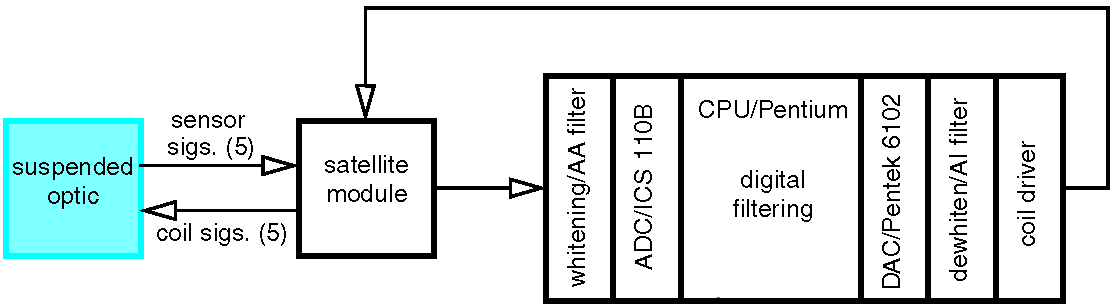
\includegraphics[angle=0,width=6.5in]{Figures/Chap5/LocalDamping.png}}
\caption[OSEM wiring]{Block diagram for the local damping electronics.}
\label{fig:SUSwiring}
\end{figure}

\begin{figure}[!h]
\centerline{
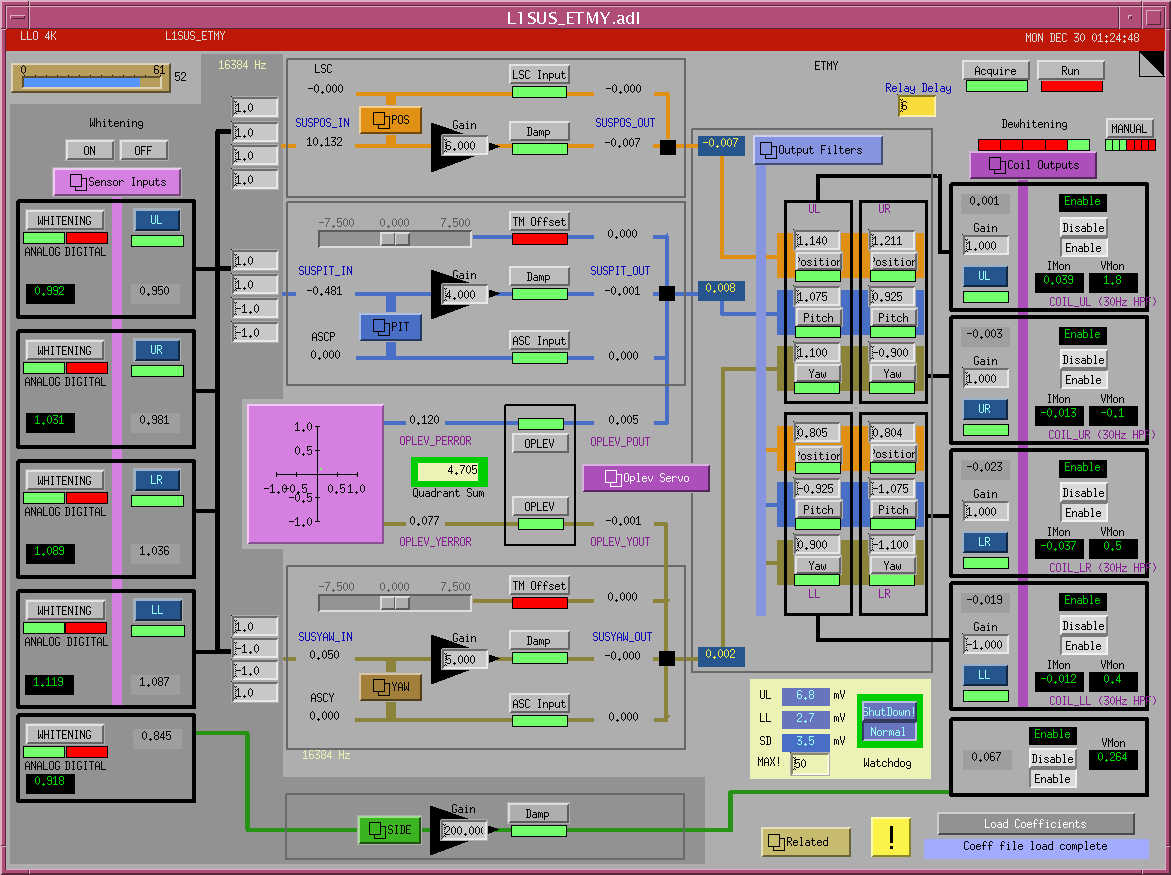
\includegraphics[angle=0,width=6.5in]{Figures/Chap5/L1SUS_ETMY.jpg}}
\caption[SUS Screen]{Overview screen for the ETMY digital suspension controls.}
\label{fig:SUSscreen}
\end{figure}

The signals from the 4 shadow sensors on the mirror face are conditioned,
acquired by an ADC, and then recombined in appropriate combinations to
reproduce signals corresponding to 3 of the free body modes of the optic.
Translation perpendicular to the optic face, pitch, and yaw are sensed
and then controlled. Vertical motion and rotation around the axis perpendicular
to the optic's face are not sensed or controlled. The sideways translation
of the optic is damped through the use of only one sensor/actuator pair.

The sensing noise of the shadow sensor 
is $\approx1 \times 10^{-10} \, \mbox{m}/\sqrt{\mbox{Hz}}$
above 20~Hz, limited mostly by shot noise in the detected light power. Since this
is 8 orders of magnitude above the displacement noise goal at 40 Hz, the filtering
must be aggressive enough to allow a gain of more than 1 for stable damping around 
1 Hz and also introduce less than 
$5 \times 10^{-19} \, \mbox{m}/\sqrt{\mbox{Hz}}$ of displacement noise at 40 Hz. 
Figure~\ref{fig:OSEMfilter} shows the open loop gain of the damping loop for
the piston degree of freedom.


\begin{figure}[!h]
\centerline{
\includegraphics[angle=0,width=6.5in]{Figures/Chap5/POSdamp.pdf}}
\caption[Pendulum Damping]{Magnitude of the open loop gain for the suspended
                           optic's piston degree of freedom.}
\label{fig:OSEMfilter}
\end{figure}




\section{Seismic Servos}
Seismic noise in the gravitational wave band affects the strain sensitivity directly by moving
the test masses. The largely unattenuated seismic disturbance below 20 Hz, 
however, is several orders of magnitude larger than the in-band noise. These 
low frequency motions impact the strain sensitivity non-linearly:

\begin{itemize}
 \item To keep the optical cavities resonant in the presence of large
   disturbances, the actuators must have a proportionally large dynamic
   range. Reducing the dynamic range with a fixed attenuator would proportionally
   reduce the noise contribution.

\item Due to the finite gain in the control servos the cavity lengths are pulled
   off of resonance, leading to bilinear up-conversion (see 
   Section~\ref{sec:residual_req} and Figures \ref{fig:POBnoise} 
   and \ref{fig:S1noiseComp} for examples).

\item There is a finite amount of light scattered at each optical surface. Some of
   this light is re-introduced into the signal readout path, producing a
   parasitic optical resonator around the main interferometer. In the regime
   where multiple wavelengths are traveled the scattered light noise can
   show up in the signal band.

\item Worst of all, often the ground noise is so large as to prevent any
   operation of the interferometer. At some point the velocities become so
   large that the lock acquisition system can no longer bring the optical
   cavities into resonance.
\end{itemize}


\subsubsection{Earth Tides}

The tidal gravitational forces from the moon and the sun distort the 
earth with a $\approx$12 hour period. These strains are
seasonally modulated, but on average create displacements of $\approx$400 
microns peak-peak over a 4 km baseline. This displacement exceeds 
the dynamic range of the test mass coil drivers ($\approx$ 10 microns).

To remove this large signal, the near DC component of the drive signals to the
end test masses' coil drivers are fed to higher dynamic range 
(180 microns peak-peak) actuators made of piezo-electric stacks. 
This system was designed to finely actuate the seismic isolation stack
at low frequencies. It is called the Fine Actuation System (FAS).

The strains from the earth tide can be divided into common and differential 
components. The common mode component can be accommodated by adjusting the 
laser wavelength as is done for the common mode servo. To accommodate 
a change, $\Delta L_{+}$, in the common mode arm length the laser 
frequency must shift by  
$\Delta \nu = \Delta L_{+} \frac{c/\lambda}{L_{arm}}$. 
This is $\simeq$7 MHz for a 100 micron length change. The slow, 
temperature actuator of the laser's master oscillator can easily give several 
hundred MHz of frequency shift.

Using an earth tide prediction program~\cite{Fred:Tides}, 
a large portion of the tidal strain was offloaded from the 
FAS in this manner on the Hanford interferometers. Figure~\ref{fig:TidalPred}
shows a comparison of the measured tidal strains with the predictions for the
Livingston interferometer during the S2 science run from February - April 2003.
From the small size of the residuals it looks like implementing the feed
forward to the laser wavelength would significantly reduce the size of the
feedback signals sent to the external seismic actuators and should be done
in the future.


\begin{figure}[!h]
\centerline{
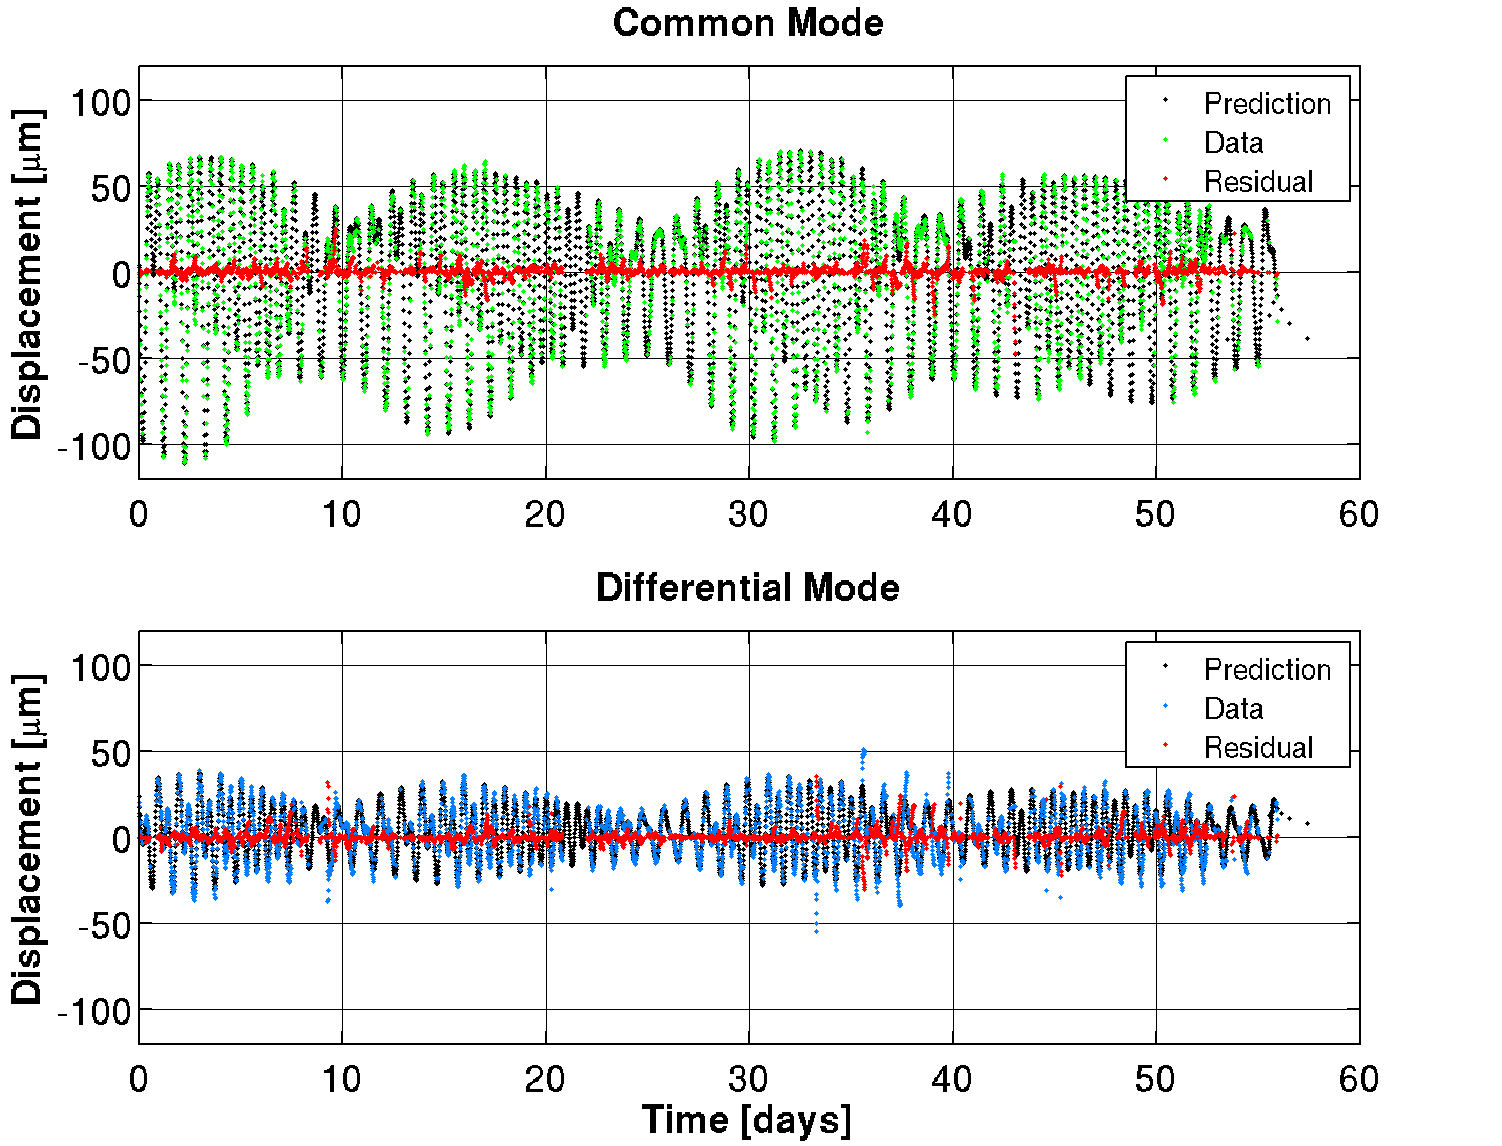
\includegraphics[angle=0,width=6.5in]{Figures/Chap5/Tides.png}}
\caption[Tidal Prediction]{The common and differential mode earth tide displacements
         are shown. Also plotted are the calibrated piezo control signals (the real
         displacements) and residual (data-prediction).}
\label{fig:TidalPred}
\end{figure}


\subsection{Microseismic Feed-Forward}

All over the earth, the largest ground motions (excepting earthquakes) are from the
$\sim$6 second period microseism discussed in Section~\ref{sec:SeismicCharacter}.

To reduce the arm length fluctuations from 0.1-0.5 Hz, a feed forward
scheme was implemented to measure the ground noise and apply this through
suitable filtering to the FAS~\cite{Giaime:MSFF}. An excellent, low frequency
seismometer (Streckheisen STS-2) was placed in each building to measure the
local microseismic motion. By measuring the displacement in each building
separately we were able to predict the microseismic arm length change and
send this signal into the second input of the FAS on the end test mass chambers 
to reduce the relative motions between the mirrors at the two ends of the arms.

Figure~\ref{fig:PEPI} shows an example of the effect of the feed forward on
the length fluctuations of a single arm cavity.

\subsection{Piezo-electric Pre-Isolator}

Out of necessity, the Livingston site was patched with 2 types of active
isolation to lower the influence of the ground motion.

As seen in Figure~\ref{fig:StackTF} the low frequency, high Q resonances of the
stack actually amplify the ground noise at some frequencies. This effect,
coupled with the large levels of anthropogenic noise, produce the large velocities
which impede interferometer operation. To reduce this effect, we installed a
local, Piezo-Electric Pre-Isolation (PEPI) system~\cite{Giaime:PEPI}.

PEPI works by sensing the sensing the horizontal velocities on the support
structure of the isolation stack and then using a stand alone computer with DSP
to feedback and reduce the seismic noise in the $\sim$0.5-3 Hz band. The
true power of PEPI comes from the digital nature of the feedback compensation.
The servo loop shape was tailored to exactly suppress the noise at the frequencies
where the isolation stack resonances would otherwise amplify. The PEPI feedback
goes into the third input of the FAS.

\begin{figure}[!h]
\centerline{
\includegraphics[angle=0,width=6.5in]{Figures/Chap5/PEPI-onoff.pdf}}
\caption[PEPI Performance]{Shows the differential arm length control signal
                   in units of velocity. The PEPI ON and PEPI OFF traces
                   show the reduction in the arm length velocities with
                   the PEPI servos on.}
\label{fig:PEPI}
\end{figure}




%-------    CHAPTER 6     -------------------------------------------
%------ Interferometer Calibration ----------------------------------------
\chapter{Calibration}
\label{chap:cal}

\begin{figure}[!h]
\centerline{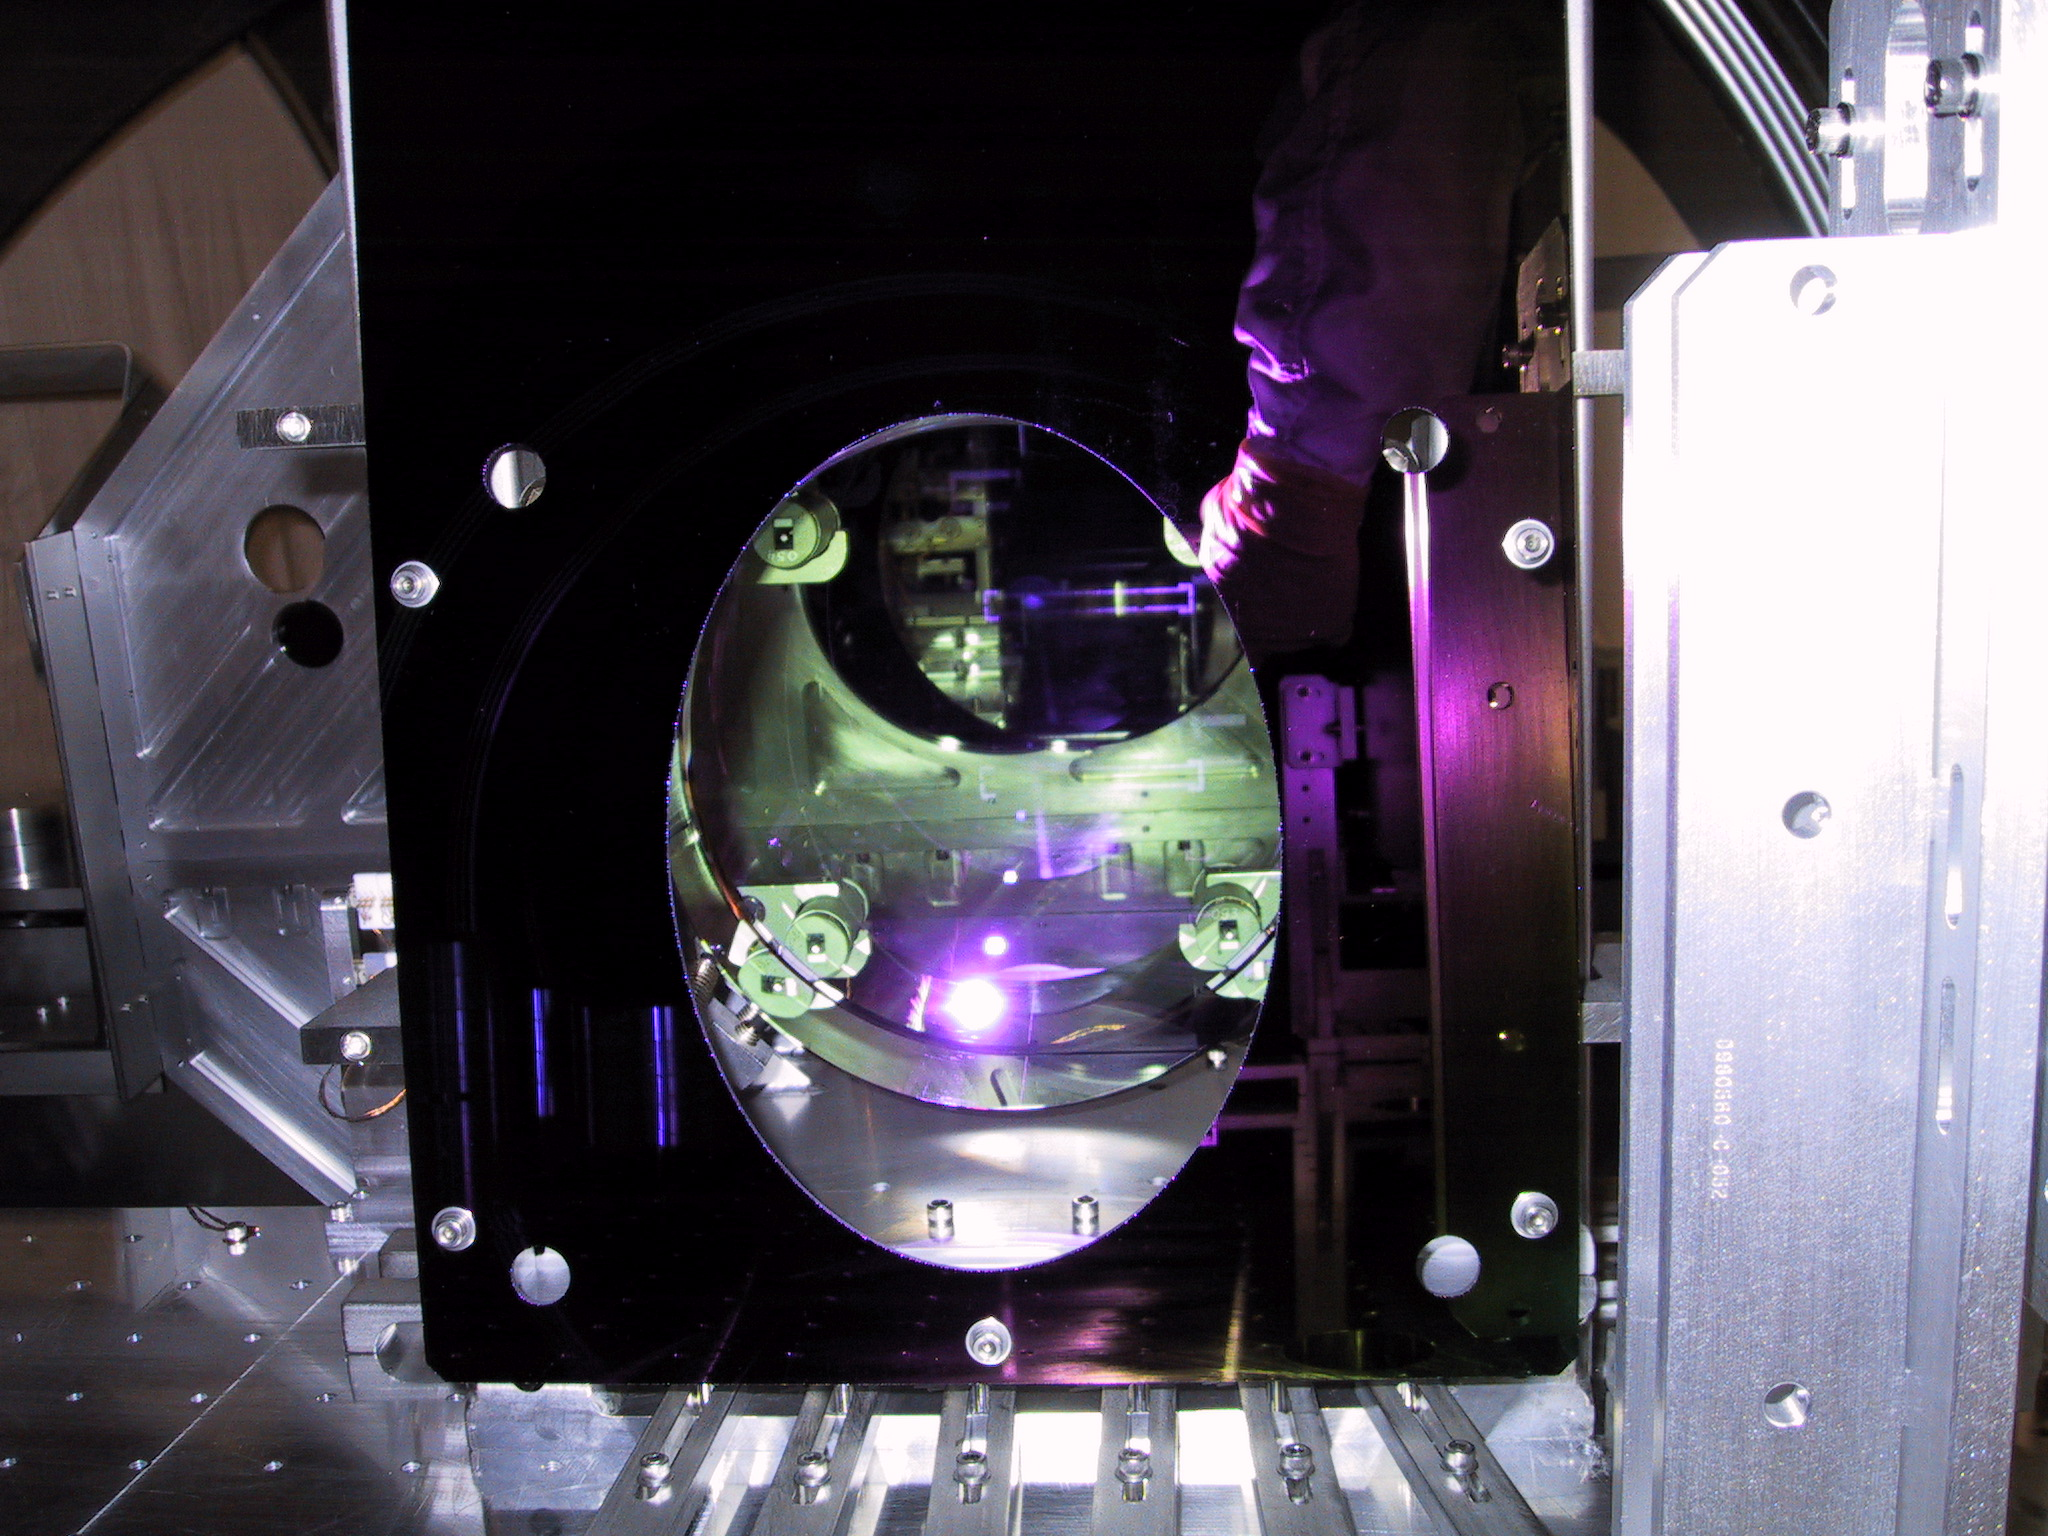
\includegraphics[angle=0,width=6.5in]{Figures/Chap6/RMfuckup.jpg}}
\end{figure}
\clearpage

This chapter describes how the interferometer's primary data channel is calibrated
to produce a measure of the gravitational wave strain incident on the 
detector~\cite{S1:Calibration,S2:Calibration}.

The interferometer output is a photocurrent which is proportional to the light power
modulation at the resonant sideband frequency ($\approx$25 MHz). We then turn this
into an integer time series after a series of analog signal conditioning
electronics. These inputs from multiple photodetectors and their electronics are
then further filtered digitally and then finally summed together to produce the
floating point time series used in the analyses. The name of the channel 
(L1:LSC-AS\_Q, H1:LSC-AS\_Q, or H2:LSC-AS\_Q) contains the following information:
the interferometer designation (L1, H1, or H2), the sub-system designation (Length
Sensing and Control), and the readout port and demodulation phase (AS port,
Quadrature phase).

This channel has the differential arm strain encoded in it. To properly decode 
this signal, 
we need to accurately determine the interferometer's \emph{response function}, 
defined as the function relating the data to the strain.


There are 3 major steps in calibrating the data:

\begin{itemize}

\item Make a model of the interferometer response (counts/meter).

\item Calibrate the mirror actuator drive (meters/count).

\item Track the calibration with a calibration line(s).
 
\end{itemize}

%------------------------------------------------------------------------------
\section{Interferometer Response Model}

The model of the interferometer's $L_-$ length control loop also serves to 
calculate the response of the DAQ channel (AS\_Q) to strains. 
Figure~\ref{fig:DARMmodel} shows a block diagram of the model and where in the
chain the data is extracted.

During standard interferometer operation, the 'Interferometer Optical Dynamics'
block, which represents the transfer function between strain and the optical
signal at the anti-symmetric port, is slowly varying (mainly due to interferometer
alignment variations).

During the S2 run, this fluctuation in the gain was uncompensated in the interferometer
control servos and led to instabilities and noise. In addition, these fluctuations
cause changes in the overall response function. Section~\ref{sec:CalLine} describes
how this is tracked.

\begin{figure}[!h]
\centerline{\includegraphics[angle=0,width=6in]{Figures/Chap5/DARM-model.png}}
\caption[L$_-$ Servo Model]{Block diagram of the model used to calculate the
         interferometer's response function. All analog circuit blocks have shadows.
         All digital blocks have orange borders.}
\label{fig:DARMmodel}
\end{figure}

The model outputs are all complex valued frequency domain transfer functions which
are supplied to all of the data analysis groups. The most commonly used product is
the response function, $R(f)$:

\begin{equation}
R(f) \equiv \frac{AS\_Q(f)}{Strain(f)}
\end{equation}


\section{Actuator Calibration}

To verify the response function given by the model, swept sine measurements are
made between the actuator and the readout in AS\_Q. To calibrate the actuator
we use the laser wavelength as the ultimate reference.

\subsection{Absolute Calibration}

A Michelson interferometer is a good displacement sensor. By misaligning the
end mirrors and the recycling mirror we get a Michelson interferometer made up
of the two arm cavity input mirrors (ITMX \& ITMY) and the beamsplitter (BS)
as shown in Figure~\ref{fig:Michelson}.

We lock the Michelson using the standard RF heterodyne readout of AS\_Q, but
limit the feedback bandwidth by putting an aggressive digital low-pass
filter in the servo loop. Then the AS\_Q signal is, in principle, directly
proportional to the differential length, $l_-$.

Since the actuator response is that of a damped pendulum with a 
$\simeq0.75$ Hz resonant frequency, it is well approximated as a
free mass in the band of interest (40-7000 Hz).

To get the absolute calibration, we have to calibrate AS\_Q in this configuration. 
To do this, we allow the mirrors to free
swing over several fringes. The peak-peak signal in AS\_Q corresponds
to a differential phase shift, $\phi_-$, of $\pi$, or correspondingly
a change in the position of a single arm mirror of $\lambda/4$, where
$\lambda = 1064$ nm, is the laser wavelength. 
So the AS\_Q calibration in ADC counts / meter is given by:

\begin{equation}
\mbox{AS\_Q cal} = \mbox{AS\_Q}_{pp}\frac{4 \pi}{\lambda} \frac{\mbox{ADC counts}}{\mbox{meter}}
\end{equation}
where this is meters of motion of a single mirror.

Systematic errors are continuously being eliminated and statistical errors
reduced through more patient measurement. The estimates on the S2 errors
are +/- 10\% in magnitude and phase~\cite{S2:Calibration}.


\subsection{Frequency Response}
To get the displacement response of the mirror to an actuation signal we measure 
the transfer function of each
piece of the mirror actuation chain shown in Figure~\ref{fig:OutputElectronics}. 
The digital compensation filters (''pre-DAC Whitening'' and 
''post-ADC un-whitening'' in Figure~\ref{fig:DARMmodel}) are constructed to
be exactly the inverse of their analog counterparts. This reduces the amount
of frequency dependent calibration error. The overall check is to again
measure the swept sine response of AS\_Q to the drive of a single mirror and
ensure that it faithfully follows the $f^{-2}$ power law of a free mass.


\section{Calibration tracking}
\label{sec:CalLine}

The variations in the interferometer optical gain are tracked by injecting a sinusoidal
drive into the digital control servo controlling the piston drive to one or both of
the arm cavity end mirrors. For the S2 run, three such calibration lines were injected 
in each interferometer: one at a low frequency ($\approx$50 Hz) where the servo 
loop gain is high, one at a frequency ($\approx$150 Hz) where the loop gain 
is $\approx$1, and one at a high frequency ($\approx$900 Hz) where the 
loop gain is low.

We use the actuator calibration to determine the amount the mirror is being
moved and monitor the amplitude and phase of the line in the data to get a 
measure of the interferometer response.



\section{Directions for the future}

There has been substantial progress in pinning down the absolute strain
calibration of the instruments and of tracking the calibration drift. The
following are some projects being pursued to further improve things:

\begin{itemize}
\item Optical gain fluctuations are currently tracked by the use of
      calibration lines and post-processing the data to correct for this. The
      real-time length control servos cannot afford such luxury, however.
      Instead, after S2, a dynamic digital gain correction was added. This
      system measures a few power levels in the interferometer and adjusts
      the digital gain in real time to correct the optical gain changes. In
      the future we should use the post-correction signal as our gravitational wave readout
      (this is the point just after the ''Input Matrix'' in Figures
       \ref{fig:DARMmodel} and \ref{fig:LSCscreen}).
      This should not only correct slow drifts in the calibration, but actually
      increase the measured strain sensitivity by removing bilinear upconversion
      from optical gain modulation at $\sim$1 second time scales.

\item The absolute calibration of the arm cavity end mirrors are now made by
      referencing them to the calibrated input mirrors. One can skip the
      intermediate step by directly referencing the end test mass drive
      to a laser wavelength shift. The laser frequency stabilization servo
      has a test input port (the AOM in Figure~\ref{fig:CMblock}) available
      for this purpose. The VCO can be directly calibrated against a spectrum
      analyzer or a high precision frequency counter.

\item It is possible to directly actuate the arm cavity mirrors through
      the radiation pressure force of an external laser. At 100 Hz, the
      displacement from a fully modulated 1 W laser at normal
      incidence is $\approx10^{-15}$ meters; quite a bit larger than
      what is currently used for a calibration line height. This radiation
      pressure calibration technique is a completely independent method to
      get the absolute calibration and avoids the complication of knowing 
      the analog filtering chain of the test mass actuators.
\end{itemize}






%-----------CHAPTER 7-------------------------------------------
%-------Ringdown Search----------------------------------------
\chapter{Data Analysis for Black Hole Ringdowns}
\label{chap:ringdowns}


\begin{figure}[!h]
\centerline{\includegraphics[angle=0,width=6.5in]{Figures/Chap1/GRB-DestroyStar.jpg}}
\end{figure}
\clearpage


This chapter describes an analysis done of the data from the second LIGO Science
Run (called S2) to look for damped sinusoid signals such as are expected from
the ringdown of black hole quasi-normal modes (see Section~\ref{sec:Ringdowns}). The
analysis was carried out over all times during which both of the 4 km interferometers were
running in their nominal data taking state.

This was an exploratory analysis, whose purpose was to answer the following questions:

\begin{itemize}

\item What is the sensitivity of the interferometers to ringdowns?

\item How much worse is the sensitivity than that of an interferometer with
      Gaussian noise of the same strain spectral density?

\item What specific things cause the sensitivity to be degraded?

\item What improvements can be made to the standard matched filter search
      as it applies to ringdowns? 

\end{itemize} 
%------------------------------------------------------------------------------
\section{Overview of the Method}

This section describes the steps involved in producing ringdown triggers from
the raw data. This part of the analysis
is similar to the analysis done by the LIGO 
Inspiral~\cite{S1:Inspiral} group.

The ringdown signals are searched for using a matched filtering code. The
matched filter templates are damped cosine waveforms which span the frequency
and quality factor (Q) space over the sensitive band of the detector and among
the Q's expected for Kerr black holes.

All of the code up to and including the trigger generation was taken from
the LIGO Algorithm Library (LAL)~\footnote{
\href{http://www.lsc-group.phys.uwm.edu/lal/}{http://www.lsc-group.phys.uwm.edu/lal/}}. 
It is C code compiled as a stand-alone executable to run on UNIX from the command line. 
For this analysis, it was sufficient to individually launch the jobs
on $\sim$10 CPU's at a time. It took $\sim$50 hours to run
the full 300 hour S2 data set for 2 interferometers using $\sim$350
templates per interferometer.

The post-processing is all done using 
MATLAB~\footnote{
\href{http://www.mathworks.com}{http://www.mathworks.com}} scripts.


\begin{figure}[!h]
\centerline{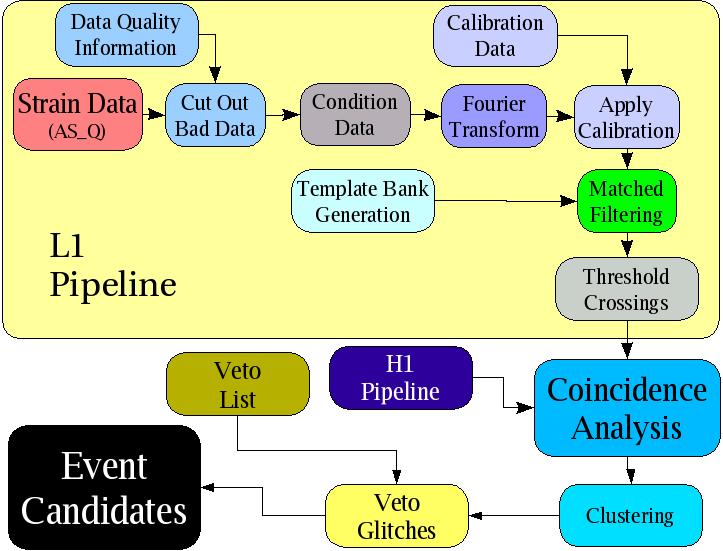
\includegraphics[angle=0,width=6.5in]{Figures/Chap7/Pipeline.png}}
\caption[Ringdown Pipeline]{The analysis pipeline.}
\label{fig:pipeline}
\end{figure}

\subsection{Matched Filtering}

The front end of the analysis pipeline uses matched filtering to produce an initial
set of ringdown triggers. Matched filtering is a commonly used technique to look
for signals of a known waveform in a noisy data stream~\cite{Bruce:MF}. A
matched filter is the optimum linear filter for the detection of a known
waveform.

We can write the calibrated detector output as a time series, $h(t)$, which is 
the sum of the signal, $s(t)$ and some noise, $n(t)$:

\begin{equation}
h(t) = s(t) + n(t)
\end{equation}
The Fourier transform of the template is

\begin{equation}
s(f) = \int\limits_{-\infty}^{\infty} s(t) e^{-2 \pi i f t} \, dt
\end{equation}
The matched filter output is

\begin{equation}
x(t) = 4 \int\limits_{0}^{\infty} \frac{s(f) h(f)}{S_n(f)} e^{2 \pi i f t} \, df
\label{eq:MF}
\end{equation}
The matched filter variance is given by

\begin{equation}
\sigma^2 = 4 \int\limits_{0}^{\infty} \frac{s(f)^2}{S_n(f)}\, df
\end{equation}
Thresholding on the signal-to-noise ratio (SNR),

\begin{equation}
\rho = x/\sigma
\end{equation}
is the optimal detection statistic for stationary, Gaussian
detector noise \cite{Jolien:40m}.

\begin{figure}[!h]
\centerline{\includegraphics[angle=0,width=6.5in]{Figures/Chap7/templatespacing_f_Q.png}}
\caption[Template Spacing (f,Q)]{Template spacing for maximum mismatch $\rightarrow$ 5\% in SNR. 
         Each dot represents one template.}
\label{fig:templates_f_Q}
\end{figure}

\begin{figure}[!h]
\centerline{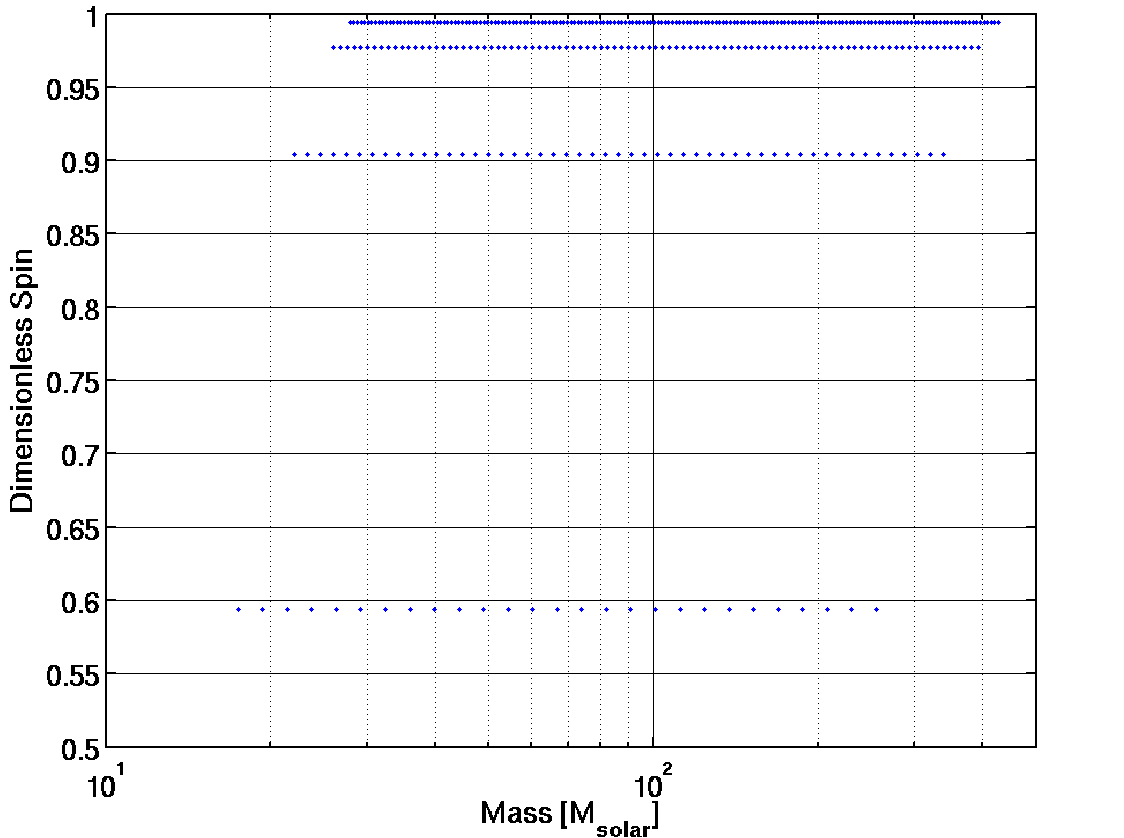
\includegraphics[angle=0,width=6.5in]{Figures/Chap7/templatespacing_M_a.png}}
\caption[Template Spacing (M,a)]{Template spacing in the (Mass, Spin) plane. These are the
                          same templates plotted in Figure~\ref{fig:templates_f_Q} 
                          but in terms of black hole Mass and Spin}
\label{fig:templates_M_a}
\end{figure}



\subsubsection{FFT the data}

The data are Fourier transformed using the Fast Fourier Transform (FFT)
algorithm, which allows the matched filter output to be calculated by
using, of order N ln(N) operations. 

\subsubsection{Inverse power spectrum}

The power spectrum which is in the denominator of Equation~\ref{eq:MF}
is estimated in nearly the same way as Welch's method: By doing a 50\% 
overlapping average of 8 data segments of length 4 seconds, but in
this case a median average is done of the segments rather than a mean
to reduce the bias from one statistical outlier.

\subsubsection{Apply calibrations}

The interferometer response function is applied to the FFT of the data
and to the power spectrum estimate. The response function is generated as 
described in Chapter~\ref{chap:cal}.

\subsubsection{Choosing the event time}

The matched filter output due to a true ringdown signal will actually cross
the threshold several times in the few hundred milliseconds around the
real start time of the signal. 

The event is localized  by clustering all threshold crossings 
within a time, 
$\tau_{dur} = \frac{10 \, Q}{\pi f}$. The time with the maximum SNR is chosen
to be the event time.


\subsection{Data Conditioning}

Before the data are examined for signals, the raw time series must undergo
some conditioning. The data are whitened and decimated.

\subsubsection{Whitening}

The raw time series of the interferometer's output spans a very large dynamic range.
The purpose of whitening the data is to prevent data corruption.
Since the data are analyzed in the frequency domain, there is the possibility
of power bleeding into adjacent frequency bins. This effect is strongest
in some of the LIGO data streams where the amplitude of the noise at low 
frequencies is several orders of magnitude larger than the noise in the
gravitational wave signal band.

Without the suppression by the servo loop, the differential arm motion
would span $\sim$13 orders of magnitude on time-scales of 10's of
seconds. With the servo on the in-loop error point at the demodulator output 
spans $\sim$8 orders of magnitude. Although this is then 
further whitened by an analog filter to fit into the dynamic range of
the ADC, this analog filter is canceled by a digital filter before the
data channel, AS\_Q, is written to disk.

Numerous schemes have been proposed to do very detailed whitening of
the data including line removal~\cite{Hua:60Hz} and linear predictive
filtering~\cite{Shourov:LPF}. For
this analysis the data was merely high-passed to remove the large low
frequency power. 

The data are filtered with a fourth order infinite impulse response (IIR) 
Butterworth high pass filter. By filtering
the data backwards and forwards, the dispersion in the filter is canceled. 
The high pass filter frequency in this analysis was set at 60 Hz, 
just 5 Hz below the frequency of the lowest frequency template.


\subsubsection{Decimation}

The data is decimated from 16384 Hz down to 2048 Hz. This is done by first
filtering with a finite impulse response (FIR) low pass filter, then by
subtracting  a time shift to compensate for the linear $d\phi/df$ from
the FIR filter, and then downsampling by the appropriate amount. The
decimation essentially reduces the analysis time by the decimation factor
since the other overhead (data retrieval, writing to disk, etc.) does
not contribute significantly to the computation time.

Preliminary runs with a 4096 Hz sample rate revealed that the number
of triggers generated by L1 above $\sim$800 Hz is enormous; as
mentioned in Chapter~\ref{chap:noise} we know that this band was
dominated by oscillator-phase noise coupling in through the highly
non-stationary RF sideband imbalance. So in that respect this low
quality data is not surprising. The large number of triggers and the
poor sensitivity above 1 kHz motivated the choice of sample frequency.

With a 2048 Hz sample rate there is no information left above the new
Nyquist frequency, 1024 Hz. By choosing this band, we are cutting
out a range of low mass black holes. From Equation~\ref{eq:RD_f}
we see that this choice loses all masses below~$\sim$10~$M_{\astrosun}$.


\subsection{Template Bank Generation}
Methods have been developed to find the minimal number of templates required to
span the templates' parameter space and yet maintain a small loss in the SNR
\cite{Jolien:40m,Owen:templates,VIRGO:templates,TAMA:templates}. The basic
idea is to use the minimum number of filters possible without losing more
SNR than some small number. By calculating the SNR loss due to a small mismatch
of waveform parameters, one can define a metric in the coordinates
relevant for the waveform; in our case frequency and Q. Using the same method
as in \cite{Jolien:40m}:

\begin{equation}
ds^2 \approx \frac{1}{8}\frac{dQ^2}{Q^2} + \frac{1}{4}\frac{dQ}{Q}\frac{df}{f}
            + Q^2 \frac{df^2}{f^2}
\label{eq:TemplateMetric}
\end{equation}
where $ds^2$ is the SNR mismatch between two templates one at (f,Q) and one at
(f + df,Q + dQ). For this analysis we placed the templates by imposing the
requirement that the maximum SNR loss be $<$ 5\%.

The number of templates is:

\begin{equation}
N_{filters} \approx \frac{1}{4 \sqrt{2}} \, \frac{Q_{max}}{ds^{2}_{max}}
                \,    \ln{\frac{f_{max}}{f_{min}}}
\label{eq:Nfilters}
\end{equation}
For this analysis, $N_{filters} \simeq 350$. With the present computing speeds available
it takes only a few days to run the analysis for 350 hours of two interferometer
data on a dozen nodes. The main bottleneck in the analysis pipeline is still the
speed of the human data analyst and not the cleverness of the tiling algorithm.

Figures \ref{fig:templates_f_Q} and \ref{fig:templates_M_a} show the templates
spacing used in this analysis in the (f,Q) plane as well as the (M,a) plane.
Almost all of the templates bunch into the region of spin from 0.9 to 1.0
since there is not much variation of Q at low to mid spin values.

 

\section{Coincidence Analysis}
\label{sec:coin_anal}

The waveform from a true gravitational wave should be almost the same as seen by both
interferometers. So to reject false events, we demand some consistency in the
waveform parameters. Each trigger is labeled by five parameters: the start
time~($t_{start}$), the SNR, the peak strain~($h_{peak}$), the frequency~($f_{ring}$),
and the quality factor~($Q_{ring}$).


\subsection{Time}

The gravitational wave arrival time difference can be as much as
11 ms between sites. With a perfect detection algorithm and noiseless
data, we could use this number as our time coincidence cut. In reality,
there is some uncertainty in the arrival time due to having a low SNR and
that there is a small mismatch between the signal and the template. It is true
that we are ultimately limited by the sample time (0.5 ms) and the relative timing
error on the two data streams ($<$ 0.1 ms), but the residual timing errors
on the simulations did not reach this level.

We empirically determine the timing uncertainty by injecting a large number 
of events in software and measuring the resulting timing error 
(see Figure~\ref{fig:ParamEst}).

\subsection{Frequency}

Similar to the arrival time cut, we can do a frequency consistency check. To cut
down on the false alarm rate, it is desirable to have the smallest
frequency cut possible, maintaining a small false dismissal
probability.

\subsection{Q}

By the same reasoning, we would like to demand a tight Q cut. 

Since the same template bank is used
for both interferometers, we are able define a coincidence as occurring only
when exactly the same template is triggered on both interferometers within the
allowed time coincidence window.

For both the f \& Q cuts, it is true that we lose some detection efficiency on
the low SNR events for which the parameter estimation is not good. However, these
events are discarded anyway \emph{because} of their low SNR.

\subsection{Amplitude}

The amplitude cut is more complicated than the other three cuts. Demanding
a strict amplitude cut requires that the relative calibration errors
between the two interferometers be small. In addition, for a true signal,
the relative antenna response functions of the interferometers must be 
taken into account (see Appendix~\ref{app:peanut} for plots of the
antenna response).

For this preliminary analysis, no amplitude cut was used.


\section{Simulations}

To test the efficacy of the entire analysis pipeline, ideally we would inject
events to mimic exactly the presence of a true gravity wave. We use the mirror
actuator (the photon calibrator will be used in the future) to move the 
test masses as a gravitational wave would. This is described in Section~\ref{sec:HI}.

Since injecting signals by hardware pollutes the data stream, we do not do
this very often. Instead, we do many simulations by adding the ringdown
waveforms directly to the data.


\subsection{Software Injections}
\label{sec:SI}

The software injections are added to the time series by taking fake,
damped co-sine waveforms, calibrating them, and then adding to the raw
uncalibrated data (just before the 'Condition Data' block in
Figure~\ref{fig:pipeline}). Then the rest of the analysis machinery
progresses in the same way as if there had not been an injection. All of the
simulations done here were done on a $\approx$10\% sample of the full data. 

\subsubsection{Parameter Estimation}
\label{sec:ParamEst}

We would like to know what the error is in determining the signal parameters.
To do this we compare the recovered waveform parameters to the intended
injection parameters.

\begin{figure}[!h]
\centerline{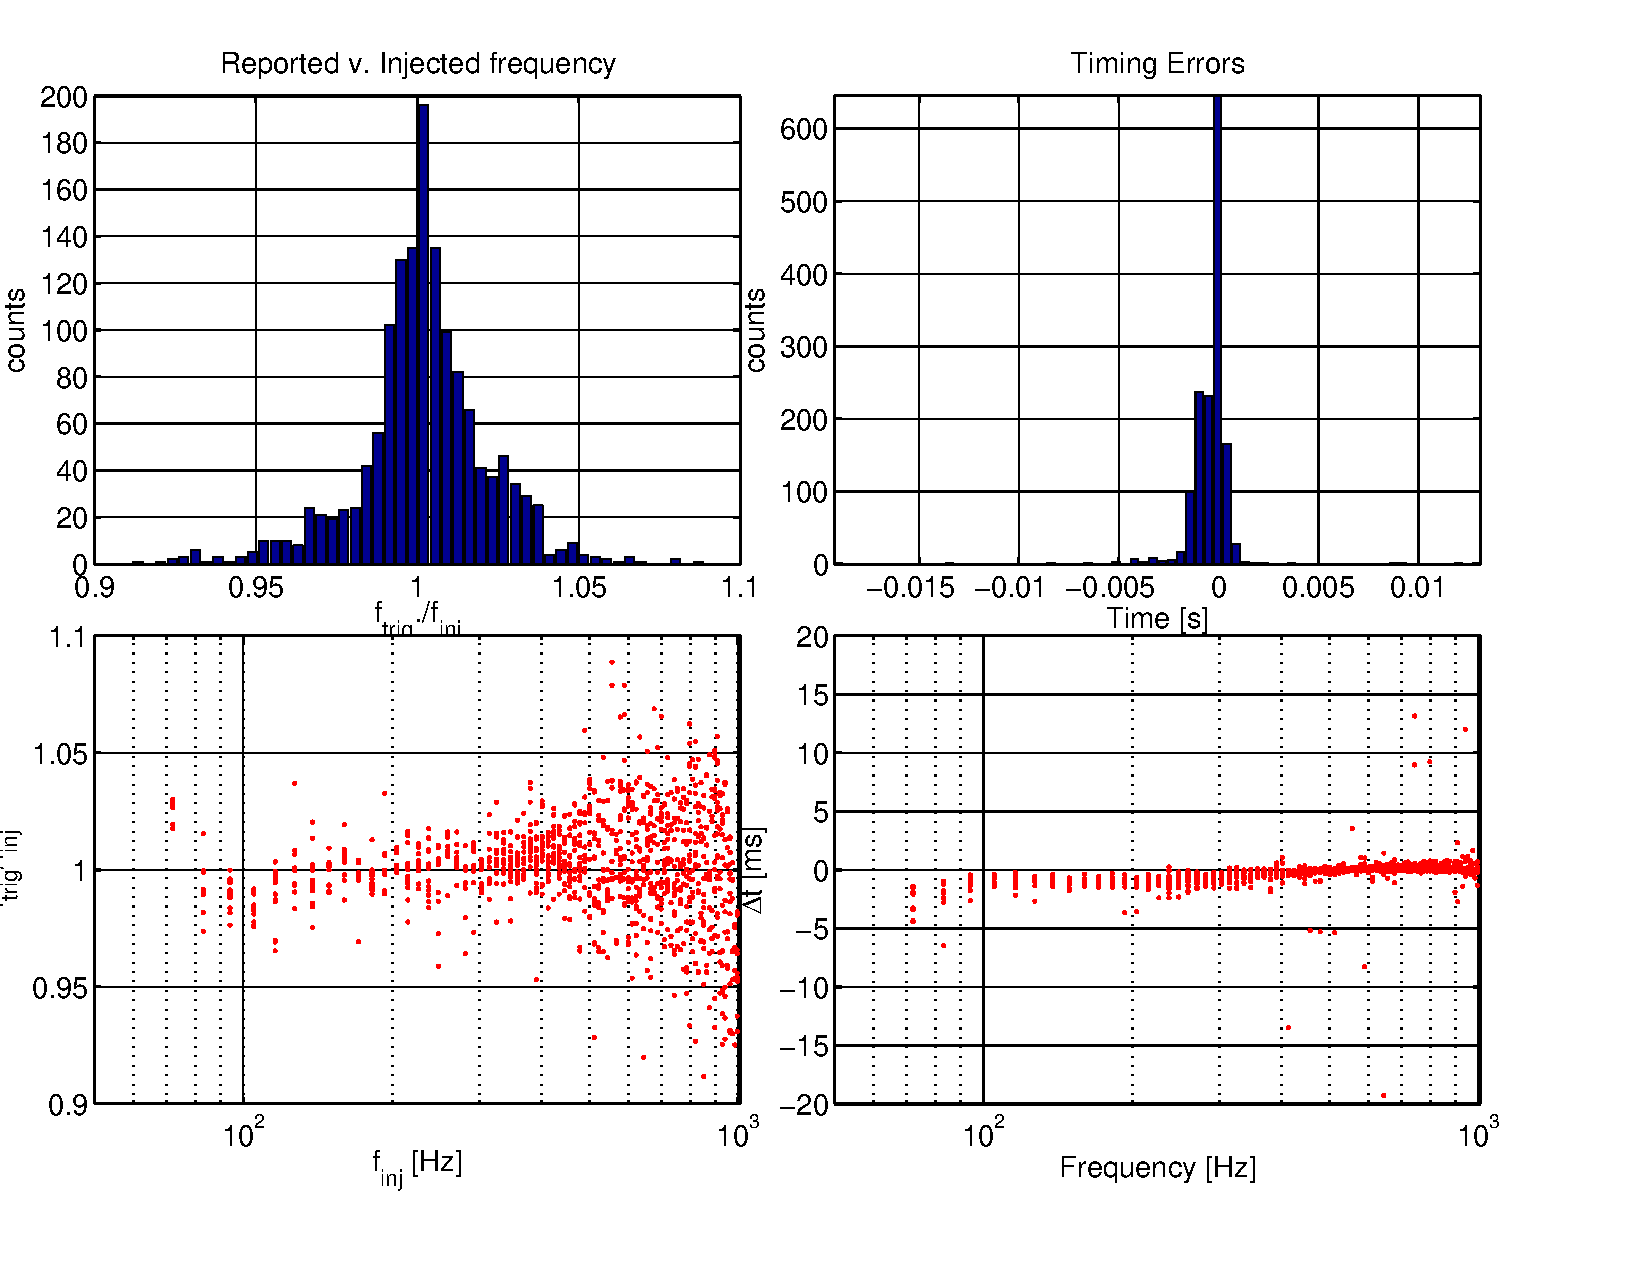
\includegraphics[angle=0,width=6.5in]{Figures/Chap7/ParamEst-Ave.pdf}}
\caption[Parameter Estimation]{Parameters reported by the pipeline versus the 
         injected parameters. In this plot the 'loudest' 10\% of the triggers
         for each event are used to estimate the trigger parameters by doing 
         an (SNR)$^2$ weighted average.}
\label{fig:ParamEst}
\end{figure}


\subsubsection{Detection Efficiency}

To interpret the results of the analysis, we measure the detection efficiency
of the software injected signals. As shown
in Figures~\ref{fig:L1efficiency} and \ref{fig:H1efficiency}, we detect almost 
all of the high SNR events and none of the low SNR
events. There is a gradual increase in the probability of detecting a signal
as the SNR is increased, which we have fit to a sigmoid function~\cite{S1:Bursts}:

\begin{figure}[!h]
\centerline{\includegraphics[angle=0,height=7in]{Figures/Chap7/eff-L1.pdf}}
\caption[L1 Detection Efficiency]{Detection efficiency of L1 as a function of peak strain. 
         The three plots show the results in 3 frequency bands. Also indicated are the 
         50\% and 90\% efficiency levels corresponding to a 50\% and 10\% false dismissal 
         probability, respectively.}
\label{fig:L1efficiency}
\end{figure}

\begin{figure}[!h]
\centerline{\includegraphics[angle=0,height=7in]{Figures/Chap7/eff-H1.pdf}}
\caption[H1 Detection Efficiency]{Detection efficiency of H1 as a function of peak strain. 
         The three plots show the results in 3 frequency bands. Also indicated are the 
         50\% and 90\% efficiency levels
         corresponding to a 50\% and 10\% false dismissal probability, respectively.}
\label{fig:H1efficiency}
\end{figure}

\begin{equation}
E(h) = \left[1 + exp(-\frac{log_{10}(h)-log_{10}(h_{50})}{a})\right]^{-1}
\end{equation}
We call the point at which there is a 50\% probability of detection,
$\epsilon_{50}$. This $\epsilon_{50}$, in terms of strain, is a function also
of frequency and Q.


\subsection{Hardware Injections}
\label{sec:HI}

Signals are also injected in real time via hardware; more to test the realism of the
software injections than anything else. The signals are calculated ahead
of time and saved into a file. The file is then loaded and the waveform is
injected into the number stream driving the longitudinal degree of freedom
of the optic. The injection point is labeled as 'EXC' in the ETMX path on 
the right hand side of Figure~\ref{fig:LSCscreen}.

Figure~\ref{fig:strainer} shows the amplitude of the injected ringdowns
compared with the noise in the detectors.

\begin{figure}[!h]
\centerline{\includegraphics[angle=0,width=6.5in]{Figures/Chap7/strainer.pdf}}
\caption[Injection Amplitudes]{The peak amplitudes of the hardware injections
         are plotted versus the noise, $h_{rms} = \sqrt{f S_h(f)}$ for the 
         three interferometers during the S2 Science Run.}
\label{fig:strainer}
\end{figure}
Comparison between the hardware and software injections is ongoing.


\section{Results}

The entire pipeline was then run on all the H1-L1 double coincident segments.
The run was done with a SNR threshold of 6 on L1 and a threshold of 5 on H1.


\subsection{Distribution of triggers}

Figures \ref{fig:hist_bands} and \ref{fig:hist_f} show the distribution
of the triggers from the individual interferometers.

\begin{figure}[!h]
\centerline{\includegraphics[angle=0,width=6.5in]{Figures/Chap7/cooter.pdf}}
\caption[Histograms of the Bands]{Amplitude distribution of the triggers in
         four separate bands. The choice of bands was made to highlight the
         different noise character in the different bands.}
\label{fig:hist_bands}
\end{figure}


\begin{figure}[!h]
\centerline{\includegraphics[angle=0,width=6.5in]{Figures/Chap7/f_hist_all.pdf}}
\caption[Number of triggers v. Frequency]{The total number of triggers per frequency
         binned logarithmically. The total number of triggers in any bin is dominated
         by the large population of low SNR events.}
\label{fig:hist_f}
\end{figure}



\subsection{Coincident Events}
After applying the coincidence criteria listed in Section~\ref{sec:coin_anal} 
there will be some remaining events; how many depends on the threshold used. 
Figure~\ref{fig:ce_hist} shows the distribution of the (L1) SNR of the 
coincident events after clustering in 100 ms chunks.

\begin{figure}[!h]
\centerline{\includegraphics[angle=0,width=6.5in]{Figures/Chap7/co_dist.pdf}}
\caption[Histogram of Coincidences]{SNR Distribution of clustered coincident events
         with SNR $<$ 50}
\label{fig:ce_hist}
\end{figure}
Since the character of the instrument noise is not Gaussian, it is difficult to 
tell if the non-Gaussian outliers are signal or noise.
 
To see if there are a statistically significant number of coincident
events within the time window determined by the light travel time
between the detectors, we re-ran the coincidence analysis many times, 
each time inserting a pseudo-random time shift in the triggers of 
one of the interferometers. Figure~\ref{fig:timelag} shows an 
example of one of these time lag simulations.

If there had been a number of real events (noise or otherwise) which were
coincident between detectors, then one would
expect there to be an excess of triggers at a lag of zero seconds. At various
thresholds and with many choices of frequency bands, there are no excess
coincident events above the level of one standard deviation above the
background.

\begin{figure}[!h]
\centerline{\includegraphics[angle=0,height=6.5in]{Figures/Chap7/lag_mid_dist.png}}
\caption[Time Lags]{Upper plot shows the number of coincident events as a
         function of artificial time lag between the interferometers. The
         lower plot shows the distribution of the upper plot. Both plots
         include only the triggers from the sensitive 150-500 Hz region. The
         L1 threshold = 10 and the H1 threshold = 5.}
\label{fig:timelag}
\end{figure}
The same plot as in Figure~\ref{fig:timelag} was made for several other choices
of threshold and frequency band, always with similar results: the number of
events at zero lag are always within 1 $\sigma$ of the background.

From these time shift plots, we can see that there is nothing special about the 
events at zero lag. In the most sensitive band (150-500 Hz), there are no
coincident events above an SNR of 9, except for two instrumental artifacts.


\section{Examination of the Remaining Coincidences}

This section looks at the coincident events at zero lag. Each event is tagged with
an event \# in Table~\ref{t:Events}.

\begin{table}[!h]
\begin{center}
\begin{tabular}{|c|c|c|c|c|c|c|}
\hline
\multicolumn{7}{|l|}
{{\bf \textsf{Event Triggers}}}\\ \hline \hline

Event \# & GPS Start Time & SNR & Strain (h$_{\mbox{peak}}$) & f &  Q & Note \\ \hline \hline

1    &  729434662.741  &    12   &   8.9e-20    &      84   &     2  & ---      \\ \hline
2    &  729531388.721  &    16   &   1.5e-19    &      78   &    17  & 60 Hz    \\ \hline
3    &  729541448.431  &    10   &   4.7e-19    &     803   &     6  & ---      \\ \hline
4    &  729920354.113  &    15   &   2.0e-19    &      65   &    21  & 60 Hz    \\ \hline
5    &  730094894.358  &    11   &   1.4e-19    &     566   &    21  & ---      \\ \hline
6    &  730133435.403  &   152   &   7.3e-18    &     994   &    21  & ADC      \\ \hline
7    &  730137174.219  &    16   &   5.0e-19    &     690   &    21  & Vio$^2$  \\ \hline
8    &  730284595.603  &    17   &   2.4e-19    &      65   &     3  & 60 Hz    \\ \hline
9    &  730285409.016  &    12   &   8.6e-20    &      94   &    18  & ---      \\ \hline
10   &  730443122.214  &    12   &   7.3e-20    &      91   &    21  & ---      \\ \hline
11   &  730443379.098  &    36   &   2.9e-19    &      80   &    11  & 60 Hz    \\ \hline
12   &  730462872.134  &    30   &   1.7e-19    &      83   &    21  & SNR       \\ \hline
13   &  730528198.849  &    13   &   8.7e-20    &      97   &    11  & ---      \\ \hline
14   &  730528295.260  &    13   &   6.2e-20    &     118   &    21  & ---      \\ \hline
15   &  730570357.681  &    11   &   2.5e-19    &     637   &    14  & ---      \\ \hline
16   &  730581701.429  &    12   &   5.0e-20    &     135   &    21  & ---      \\ \hline
17   &  730592358.344  &    12   &   8.0e-20    &      87   &    11  & ---      \\ \hline
18   &  730605715.704  &    10   &   3.7e-20    &     136   &    21  & ---      \\ \hline
19   &  730669046.827  &    10   &   1.0e-19    &      80   &    21  & ---      \\ \hline
20   &  730881699.750  &   132   &   4.7e-19    &     180   &    21  & ADC      \\ \hline
21   &  732581991.246  &  1580   &   5.4e-17    &     734   &    11  & ADC      \\ \hline
22   &  732637065.650  &    11   &   7.7e-20    &     119   &    11  & ---      \\ \hline
23   &  732639925.100  &    14   &   5.0e-19    &     848   &    17  & ---      \\ \hline
24   &  733037033.244  &    71   &   6.1e-19    &     353   &    21  & Violin   \\ \hline
25   &  733037804.016  &    15   &   6.4e-20    &     112   &    21  & ???      \\ \hline
26   &  733592255.881  &    11   &   2.4e-19    &     695   &    21  & ---      \\ \hline
27   &  733749193.282  &    13   &   2.1e-19    &     669   &    18  & ---      \\ \hline
28   &  733751635.889  &    15   &   7.8e-20    &      78   &    21  & ---      \\ \hline
29   &  734139127.398  &    13   &   8.5e-20    &      78   &    16  & ---      \\ \hline
30   &  734149435.240  &    12   &   5.8e-20    &      94   &    21  & ---      \\ \hline 
\end{tabular}
\end{center}
\caption[Coincident Events in S2]{Parameters for the coincident events in S2 with
                                  SNR $>$ 10}
\label{t:Events}
\end{table}

\subsection{Study of the Remaining Events}

The coincident events with a SNR in L1 above 10 were examined 'by hand'
by looking at the time series plots after bandpassing the data in a few hundred Hz
band around the trigger's central frequency.


\subsubsection{Event \#21 - SNR = 1580}

Event \#21 is an ADC saturation. The AS\_Q time series that we record is a digitally
processed version of the raw ADC inputs. To determine what the ADC recorded we apply
the inverse of that digital processing. Applying this procedure to \#21 we see that the
ADC signal suddenly rails several times at +32767 and -32768. The signal then recovers
and the interferometer resumes normal operation.

During the course of the run several of these events were observed and more often than
not these saturations caused a loss of lock. This was tracked down to be a malfunctioning
piece of electronics; voltage noise on the gain control of the AS port whitening board
caused fast steps in the AS\_Q ADC signal. 

Following the S2 run, software monitors were put in place to record all ADC saturations
and the flagged data have been vetoed. Even better, a new design for the whitening 
electronics uses a TTL logic control for the gain command, eliminating this type of 
malfunction.


\subsubsection{Event \#6 - SNR = 152}

This one is another ADC saturation, although of a different nature. Just below the
sensitive 70-1000 Hz band is a large 'wall' of noise which is of a seismic nature,
although not the standard seismic coupling mechanism. It comes from a variety of noise
sources including mechanical resonances of the optical lever piers, unfiltered
electronics noise from the wavefront sensors, and in this case, nonlinear upconversion
of the $\sim$ bounce mode of a suspended large optic. During the run, we noticed that
ground noise due to some malfunctioning HVAC equipment would excite the mechanical
modes of several optics. Large amplitude signals (through some unknown mechanism)
would also produce a large component at 3$\times$ the fundamental frequency. This
large signal at $\sim$35 Hz is then amplified by the analog whitening filter.

The RMS from this signal is several times smaller than the ADC range, but statistically
we expect to see a large excursion once in awhile. These excursions can either cause
a loss of lock or, as in this case, produce a strong glitch.

Based on these experiences, a new whitening filter design was implemented before the
next science run. The new whitening filter has $\sim 4 \times$ less gain in this
noisy band. In addition, there are some efforts to fix noisy HVAC equipment.


\subsubsection{Event \#20   SNR = 132}

Another ADC saturation. Essentially the same behavior as Event \#6.


\subsubsection{Event \#24   SNR = 71   f = 353 Hz}

Nothing in H1. A sudden sharp transient in L1. The template frequency
is the same as that of one of the test mass violin modes, but it is not
clear if this is a coincidence or not.


\subsubsection{Event \#11   SNR = 36  f = 80 Hz}

Looks like some transient upconversion around 60 Hz. It is only a small
increase in the RMS of the 60 Hz shoulders; this is a common occurrence
and this $\sim$20 Hz band around 60 and 120 Hz often show this
non-stationary behavior.


\subsubsection{Event \#12   SNR = 30  f = 83 Hz}

Interesting looking glitch in L1, but at too low of a level to show up
in the bandpassed H1 or H2 time series.

\subsubsection{Event \#8   SNR = 17   f = 65 Hz}

Just like \#11. 60 Hz junk.


\subsubsection{Event \#7   SNR = 16   f = 690 Hz}

A random fluctuation in the 2nd harmonic of a violin mode in both interferometers.
It seems like the data in a small band around the first and second violin mode
harmonics is constantly getting rung up. If this cannot be suppressed by
further notching in the control servos, it may be necessary to ignore all the
triggers from these bands.


\subsubsection{Event \#2   SNR = 16   f = 78 Hz}

L1 AS\_Q goes to +/- 20000 ADC counts but does not saturate. Looks like a
35 Hz and 60 Hz problems evident in events \#6 and \#11.


\subsubsection{Event \#4   SNR = 15   f = 65 Hz}


\subsubsection{Event \#25   SNR = 15   f = 112 Hz}

There is nothing visible in the time series above the background.



\section{Future Improvements}

This analysis is a preliminary attempt to look for ringdown signals with the
main emphasis being on uncovering gross problems or difficulties. As such,
there a number of ideas / methods / techniques which were not implemented
yet but are listed here for posterity.

\begin{itemize}

\item It seems clear that the burden is on the commissioning team to
      reduce the large variability in the noise floor and the high rate 
      of transients. A noble goal would be to reduce the rate of transients
      until the random double coincident rate meets the expectations from
      Poisson statistics up to SNR$= 15$. Efforts are underway to develop 
      a 'ringdown' monitor
      program to run in the control room at both sites to give a feel for
      the variability of the false rate as instrument parameters are adjusted
      during commissioning of the interferometer.

\item A method needs to be developed to veto non-ringdown events which cause
      the templates to exceed threshold. One method may be examining the software 
      injections to determine the amplitude and start times in neighboring
      templates\cite{Jolien:40m}. A true ringdown signal should have a well 
      defined distribution
      in template space. One has to be careful not to veto a potential
      merger-ringdown signal by placing too tight a criteria.

\item Do a direct waveform consistency check by cross-correlating the
      interferometer outputs in the neighborhood of the events. This is
      a technique currently being developed for detecting unmodeled 
      bursts~\cite{Laura:Rstat}.

\item Do a real Monte-Carlo simulation over the matched filter and 
      coincidence parameters to optimize the search sensitivity.

\end{itemize} 


\section{Conclusions}

A preliminary search was done for damped sinusoids in the data. The search
highlighted several problems in the interferometers and in the search method.

The equivalent strain amplitude of the coincident events at SNR of 10
agrees with the rough estimate made by comparison with noise spectral density.

It is clear that more simulations will have to be done to determine precisely
the detection efficiency as a function of time for each interferometer. A method
of vetoing the non-ringdown triggers needs to be developed to reduce the
false rate.







%-------    CHAPTER 8     -------------------------------------------
%------ Future Improvements ----------------------------------------
\chapter{The Future}
\label{chap:future}

\begin{figure}[!h]
\centerline{\includegraphics[angle=0,height=5.5in]{Figures/Chap8/Porcupine.png}}
\end{figure}
\clearpage



%------------------------------------------------------------------------------
\section{Possible Future Improvements}

At present none of the three interferometers operates at the designed sensitivity
level. In addition, the duty cycles (especially of the Livingston detector) are
not at the 90\% level which they were designed for. The following are some ideas
for improving the state of affairs. Some are currently being explored and some only
exist on paper.


\subsection{Seismic Isolation}
During the course of this writing, a scheme has been developed for mitigating the
excess seismic noise which limits the duty cycle and data quality of the Livingston
interferometer.

Quiet hydraulic actuators~\cite{Giaime:AdvIso} with collocated sensors are being 
installed on the existing seismic isolation support structure. This system,
the Hydraulic External Pre-Isolator (HEPI), is also intended for the Advanced LIGO upgrade.

Since the in-vacuum, passive isolation stack has various cross-couplings (e.g. from
pitch to horizontal motion), the HEPI is designed to reduce the vibration in all 6
DOF on the outside of the vacuum chamber. Preliminary testing indicates that the
HEPI performance will exceed the factor of 5-10 reduction in broadband displacement
noise which was the goal.

The Hanford site seems to be sufficiently quiet (with the exception of occasional
periods of high winds), such that at present, no such drastic retrofit is planned.
However, the dramatic success of HEPI could make the Hanford sites ground noise
seem egregiously large in comparison to the isolated Livingston platforms.


\subsection{Output Mode Cleaner}

The current interferometers have many problems associated with poor beam quality or
imperfect interference at the interferometer's dark port:

\begin{itemize}
\item Excess carrier light at the dark port produces excess shot noise.

\item The reflectivity difference of the two arms will produce a static, TEM$_{00}$,
      carrier field at the dark port. This static field beats with noise on the
      sideband light to produce noise in the signal channel.

\item The portion of the sideband field which does not spatially overlap with
      the carrier does not contribute to increasing the optical gain. Instead,
      it produces many junk effects: shot noise, acoustic sensitivity, jitter
      sensitivity, etc.
\end{itemize}

One solution to these problems which is being currently pursued is the use of an
output mode cleaner. This would be a short, rigid, triangular cavity placed on
the anti-symmetric port output table. Such a short ($\sim$5 cm), low 
($\sim$ 30) finesse cavity would have large enough linewidth to transmit the 
RF sidebands and the carrier in the same resonance. Higher order spatial modes, 
however, would be passively rejected just as in the input mode cleaners. 
The suppression of the higher 
order spatial modes is given by Equation~\ref{eq:ModeCleaning}.

Once the the contrast defect due to higher order modes has been effectively
removed, one can re-optimize the SNR by adjusting the modulation depth for
the resonant sidebands as described in Section~\ref{sec:darksignals}.


\subsection{Thermal Compensation}
\label{sec:ThermalComp}

A serious problem with the interferometers is the unstable nature
of the power recycling cavity. 

The power absorbed by the optics forms a thermal lens in the bulk of the glass
through the temperature dependence of the index of refraction. The original design 
planned on a precise amount
of thermal lensing and pre-polished the power recycling mirror to account for this.
Preliminary estimates indicate that the absorption levels vary substantially
from optic to optic. 

The carrier mode in the recycling cavity is determined by the average spatial mode
of the arms and so the carrier field is largely immune to curvature errors in the
recycling cavity. The sideband fields are not resonant in the arms and so the
mode matching of the sideband to the recycling cavity depends critically on the
amount of thermal lensing. The experience with the interferometers so far has
shown that it will be necessary to control the recycling cavity resonant mode
to keep it well matched to the arms. 

The three most deleterious consequences of the unstable recycling cavity are:

\begin{itemize}
\item The RF sideband is not spatially mode-matched to the recycling cavity. 
      So most ($\approx$90-95\%) of the sideband power is reflected from the
      recycling cavity. This
      results in low optical gain at both the recycling cavity pickoff and 
      anti-symmetric ports.

\item The RF sideband field which does make it to the AS port does not overlap
      well with the carrier field and therefore the gravitational wave signal sidebands. This
      means that much of the RF sideband field which is there contributes 
      to increased shot noise and not to the signal strength.

\item The unstable nature of the PRC results in large optical gain modulation
      for small angular fluctuations. This leads to instability in all of the
      conditionally stable servo loops.
\end{itemize}

To compensate for the lack of thermal lensing, a system, initially intended
for Advanced LIGO~\cite{Ryan:Thesis}, is being commissioned to
stabilize the cavity. By applying the correct spatial distribution of heat 
to each ITM, one can induce a thermal lens in the test mass bulk. This will
pull the recycling cavity from unstable to marginally stable. 

The plan is to heat each ITM with a CO$_2$ laser with a fixed mask to shape 
the heat distribution. The Nd:YAG laser power will be turned up all the way 
and the CO$_2$ beam will be adjusted accordingly to maximize the SNR of the
$\delta L_{-} \rightsquigarrow AS\_Q$ readout.


\subsection{Oscillator Phase Noise}

During the course of commissioning, a strange and large sensitivity to phase
noise on the RF oscillator was measured. This noise source dominates the 
interferometers' noise budgets above 1 kHz.

While the source of the coupling is not established as of yet, it is believed
that reducing the phase noise of the oscillator itself will partially
mitigate the problem. In the near future low noise, crystal oscillators will
be installed. These oscillators have a narrow tuning range compared to the
existing frequency synthesizers, but have a SSB phase noise of -165 dBc/$\sqrt{\mbox{Hz}}$
at 1 kHz (as compared to the -150 dBc/$\sqrt{\mbox{Hz}}$ of the currently installed units).


\subsection{Laser Frequency Noise}

\subsubsection{A Better Frequency Reference}
As shown in Figure~\ref{fig:CMnoise}, the overall frequency stabilization
factor would be almost good enough except that the noise in our frequency
noise readout channel is too high to produce a quiet laser beam. The main
work that needs to be done is to reduce the shot noise limited sensitivity
at that port.

Until now we have been using a signal readout scheme where each length
signal is constructed by demodulating at the resonant sideband frequency.
Unfortunately, this causes us to suffer problems similar to those experienced
at the AS port with junk light. The uncontrolled Q phase signal in reflection
dominates, by a few orders of magnitude, the I phase signal used to readout
the $L_{+}(f)$ or $\nu(f)$ signal. This limits the total amount of light we can
detect without saturating the RF photodetector. At such low levels ($\sim$1 mA,
30X smaller than designed) the shot noise limit is quite high.

An alternative scheme is to use the non-resonant sideband (which is already used
for angular sensing). Whereas the resonant
sideband level at the reflected port is slowly extinguished as the recycling
cavity is thermally lensed, the non-resonant sideband is, in principle, unaffected
by the state of the recycling cavity and can produce a strong signal, largely
independent of the problematic recycling cavity. There is also no Q phase signal 
expected at the non-resonant sideband frequency, in principle.

\subsubsection{More Loop Gain}

Above a few kHz, the frequency noise exceeds its designed noise level. The result
is that the interferometer sensitivity would be compromised at high frequencies
once the other noise sources are reduced.

The reason for this high frequency excess is that early in the commissioning phase
for the Mode Cleaner, the servo loop gain was reduced to make the servo more
stable. In this low gain state the VCO phase noise dominates the MC noise 
(see Figure~\ref{fig:MCnoise}) and this propagates into the interferometer.

Some combination of higher loop gain in the MC and a quieter VCO will have to
be explored in the future to meet the noise requirements.


\subsection{Wavefront Sensing}
\label{sec:WFSfuture}

At the time of this writing, the full Wavefront Sensing (WFS) and angular control
system has been demonstrated to work on all the interferometers, although it
has only stably operated on the Hanford interferometers.

In order to have some day to day stability and consistent data quality, it is
vital that this system work on all interferometers. In the near future it is
envisioned that the WFS system will be commissioned in Livingston to bring it
to the level of the Hanford instruments.

On all the interferometers, there remains substantial work to be done on the
electronics for this system to reduce the noise contributed to the gravity
wave channel. The reduced noise will allow operation with higher gain. 
There does not seem to be any fundamental roadblock here.


\subsection{Increased Laser Power}

In the past few years of detector commissioning, the laser power into the
interferometer has been run, usually, at lower power than designed for. 
This is due to a number of reasons:

\begin{itemize}
\item Low transmission through the optics between the laser and the interferometer.
\item Unintentional low power due to degraded Power Amplifier pump diodes, poor amplifier
      alignment, or low power from the master oscillator.
\item Intentional low power from the laser by lowering the pump diode current to extend
      diode lifetime.
\item Not being able to handle high power in the interferometer itself (scattering,
      radiation pressure, wimpy photodetectors, etc.)
\end{itemize}

Efforts are now underway to chip away at this power deficit by better alignment,
mode-matching through the PMC, increased pump power, etc. It looks promising that
there soon can be the full 6 Watts of power entering the interferometer.

A hypothetical question to pose is, what can be done to further increase the
laser power by another factor of 2-5. Some concepts to quantitatively explore
over the next two years are:

\begin{itemize}
\item Increase the power output of the master oscillator. Currently we are
      pumping the NPRO master oscillators at $\sim$500 mW. At this power level
      the PA is only partially saturated and so while doubling the MO power
      will not double the MOPA power, we should explore how much this will give.

\item Add another amplifier. By taking the MOPA output and putting it through
      a single pass, commercially available amplifier or another double-pass
      PA like we have now would make a much more powerful laser; a MOPAPA.

\item Convert the PA into a ring cavity and injection-lock it to the NPRO.
\end{itemize}

\subsection{Low Noise DAC}

The noisy digital-to-analog converters currently used require us to use
aggressive, complex analog filtering to both achieve low displacement noise
and yet have enough range to accomodate the low frequency seismic noise.

The development and testing of DACs with $\sim$30X less noise is being
pursued. These would lower the influence of DAC noise below the SRD/10 level
in all interferometers and also allow one to rework the post-DAC filtering
to give increased dynamic range.

\subsection{Sweet Spot on the Suspension}
\label{sec:sweetspot}

The estimate made for suspension thermal noise in Section~\ref{sec:SUSthermal}
assumed that the beam was centered on the test mass. This is not the position
in which the suspension thermal noise is minimized.

It was recognized several years ago \cite{Gaby:Thermal,Levin:SUSthermal} that 
there is a 'sweet spot' on the
optic which minimizes the thermal noise. When the test mass pendulates, most
of the loss is due to bending in the wire at the top suspension point and at
the bottom of the wire, near where it contacts the optic (see Figure~\ref{fig:SUS}). 
By symmetry, only the thermal forces generated at these two points affects the 
test mass motion.


For the thermal forces generated at the bottom of the wire, there is a node
in the optics motion slightly below the center of mass. By adjusting the cavity
axis so that the beam resonates at this point, one can make the measured
interferometer strain noise insensitive to the this thermal noise and only
sensitive to the loss in the top of the wire.

Following the method of \cite{Gaby:Thermal} we can get a numerical result and
find that the minimum is $\sim$1 cm below the center of mass. In the case where
suspension thermal noise is the only noise in that band we can get a $\sim$20\%
reduction from $\sim$50-100 Hz.


\subsection{Low internal mode noise}

Between the time the interferometers were designed and the present, the state-of-the-art
in thermal noise modeling has crept forward somewhat. In particular, it has been
recognized that the substrate thermal noise should be less than what was assumed
in the initial design and that coating thermal noise is approximately equal to
the substrate thermal noise for the LIGO-I choice of beam parameters and coating
materials.

In particular, it appears that the overall test mass thermal noise will come out
$\sim$2X smaller than was expected originally.
 

\subsection{DC Readout}
\label{sec:DCreadout}

In the current signal readout scheme, the GW signal is encoded as 
an amplitude modulation on the RF carrier (which is itself generated as a
beat between an optical frequency carrier and an RF sideband). This method
has a historical origin; in the 20$^{th}$ century, the amplitude and
phase noise on commercial lasers was so bad that there was no hope of
reaching the shot noise limit at the audio frequencies where GW's are
expected.

Recently~\cite{Peter:DCreadout} it has come to light that this is no 
longer the case. The combination of quiet, solid-state lasers with
the high-gain, low noise, amplitude and frequency stabilization servos
already significantly reduces these noises. The advantage to eliminating
the RF sidebands, however, is revealed through the way the laser noise
couples into the interferometer. As described in Sections
\ref{sec:IntensityNoise} and \ref{sec:FreqNoise}, the RF sidebands do
not experience the $\sim$1 Hz low pass filter of the full coupled
cavity resonance that the carrier does and so eliminating them
would reduce the coupling from laser amplitude and frequency noise
and of course, completely eliminate oscillator based noises.

Instead of reading out the signal by doing a phase modulation on the
input beam, one can just shift the differential arm length slightly,
yielding a first order change in the AS port power as a function of
differential arm length.

There are a few other advantages to employing a DC readout:

\begin{itemize}
\item Exploring the possible space of modulation/demodulation waveforms
      \cite{Meers:modulation}, we know that the theoretical best SNR
      is achieved by using no modulation or demodulation. 

\item Even better than the fact that it is the theoretical best, is the
      fact that it guarantees perfect overlap between the local oscillator
      and signal fields: The 'LO' in this case is just the static
      carrier generated by the intentional arm length offset.

\item Instead of all of the complicated electronics associated with an
      RF readout, one can just readout the DC power on the photodiode.
      With an Output Mode Cleaner this requires only a few mW total.
\end{itemize}




\section{Estimating the future performance}

In the past, predictions about the detectors' noise performance have had a mixed
level of accuracy. It is certainly true, however, that the predictions have gotten 
more accurate as the noise is reduced and the instrumental characterization becomes
more advanced.

Determing the ultimate sensitivity of the detectors is of great interest, since
we would like to know sooner than later if some major upgrade or redesign will
be required to reach the design sensitivity.

The initial LIGO design curve was made $\sim$15 years ago, based upon the
knowledge available at that time. Now that the interferometers are built we
are able to make more accurate estimates of many of the parameters involved
in generating these noise curves. There are three particularly important cases:

\begin{itemize}
\item The initial design noise curve was dominated at the $\sim$150 Hz minimum
      by thermal noise in the mirrors. The loss in the mirrors appears to be 
      10X less than expected. This makes the thermal noise from the mirror 
      substrate 3X less than the design.

\item The interferometers' contrast defects are all 20-100X better than the
      conservative estimate made in the design. This gives a reduced level of
      shot noise which dominates above 200 Hz.

\item After the initial design, it was recognized that the true mechanism for
      suspension thermal noise gave a steeper frequency dependence and so the
      suspension thermal noise contribution is much less above the pendulum
      resonance frequency.
\end{itemize}

As shown in Figure~\ref{fig:S5noise}, I predict that the sensitivity of the initial
interferometers will significantly surpass the design, as long as we are able to
reduce the technical noise sources to their initial design levels and no
unforseen, insurmountable noise sources are discovered.

 
\begin{figure}[!h]
\centerline{
  \includegraphics[angle=0,width=6.5in]{Figures/Chap8/s5noise2.pdf}}
\caption[S5 Noise]{Best possible noise curve using the existing IFO components. The significant
                   sensitivity improvements from using a DC readout and higher laser power
                   are not shown.}
\label{fig:S5noise}
\end{figure}




%
%
%     CONCLUSION
%
%
%------------------------------------------------------------------------------
\chapter*{Conclusion}
\addcontentsline{toc}{chapter}{Conclusion}

The sensitivity of the LIGO interferometers continues to improve, almost monthly,
due to a large concentrated effort by the detector commissioning team. The
noise floor has been reduced by 6 orders of magnitude in the last few years
and is now less than a factor of 10 away from the initial sensitivity goals.

Vital to the noise reduction effort has been the modeling of the interferometer's
response to noise coming from all significant sources.

A simple analysis has been done of two months of data from one of the LIGO science
runs for damped sinusoid signals. The sensitivity of the detectors to this type
of signal was seen to be degraded by the non-Gaussian noise character of the
interferometers and there are good ideas for future work.

A number of options have been outlined for near term upgrades to the interferometer.
It is expected that implementing these fixes would let us exploit the true
astrophysical reach of these instruments, surpassing the initial expectations
of the sensitivity by a factor of 3.

\clearpage


% Header for all appendices. Need just once.
\appendix
\addcontentsline{toc}{chapter}{Appendices}

%-------Appendix A-------------------------------------------------------------
%-------Tables of Parameters---------------------------------------------------
\chapter{Tables of Parameters}
\label{app:Parameters}

%-------Fundamental Constants ---------------------------------------------------
\begin{table}[!h]
\begin{center}
\begin{tabular}{|l|c|c|c|}
\hline
\multicolumn{4}{|l|}
{{\bf Physical Constants}}\\ \hline \hline
Parameter                 & Symbol      & Value                    & Units   \\ \hline \hline

Speed of Light               & $c$         & 299792458                & m/s         \\ \hline

Planck's Constant            & $h$         & $6.6261 \times 10^{-34}$ & J s         \\ \hline

Boltzmann's Constant       & $k_B$       & $1.380 \times 10^{-23}$  & J/K           \\ \hline

Electron Charge              & $e_c$       & $1.602 \times 10^{-19}$  & C           \\ \hline 

Gravitational Constant    & $G$         & $6.674 \times 10^{-11}$  & m$^3$/kg/s$^2$ \\ \hline

Fine Structure Constant      & $\alpha$    & 1/137.036                & -            \\ \hline

Stefan-Boltzmann Constant   & $\sigma_B$  & $5.67 \times 10^{-8}$    & W/m$^2$/K$^4$ \\ \hline

Avogadro Constant           & $N_A$       & $6.022 \times 10^{23}$   & mol$^{-1}$    \\ \hline

\end{tabular}
\end{center}
\caption[Fundamental Constants]{Values of constants from the NIST 
                                CODATA webpage \cite{CODATA}}
\label{t:Fundamental}
\end{table}



\begin{table}[!h]
\begin{center}
\begin{tabular}{|l|c|r|c|}
\hline
\multicolumn{4}{|l|}
{{\bf Large Optic Parameters}}\\ \hline \hline
Parameter                         & Symbol     & Value             & Units   \\ \hline \hline

Specific Heat		             & $c_H$        & 740               & J/kg        \\ \hline

Refractive Index (@ 1064 nm)         & $n$        & 1.45              & -           \\ \hline

Thermal Conductivity 	             & $k$	  & 1.38    & W m$^{-1}$ K$^{-1}$   \\ \hline

Young's Modulus	(substrate)	     & $Y_S$      & 72.80	      & GPa         \\ \hline

Young's Modulus	(coating)	     & $Y_C$      & 100	              & GPa         \\ \hline

Poisson Ratio		             & $\sigma$   & 0.170	      & -           \\ \hline

Thickness (coating)           & d$_C$      & 8 $\times$ 10$^{-6}$     & m           \\ \hline

Loss Angle (substrate)            & $\phi_S$  & 1 $\times$ 10$^{-7}$  & -           \\ \hline

Loss Angle (coating)                 & $\phi_C$   & 2 $\times$ 10$^{-4}$ & -        \\ \hline

Density		                     & $\rho$     & 2196              & kg/m$^3$    \\ \hline

Optic Radius             & $R_{\mbox{\tiny LOS}}$     & 0.125         & m           \\ \hline

Optic Diameter                       & dia        & 0.250             & m           \\ \hline

Optic Thickness             & $h_{\mbox{\tiny LOS}}$   & 0.100        & m           \\ \hline

Optic Thickness (BS)        & $h_{\mbox{\tiny BS}}$    & 0.040        & m           \\ \hline

Optic Mass              & $m_{\mbox{\tiny LOS}}$  & 10.5              & kg          \\ \hline

Optic Mass  (BS)          & $m_{\mbox{\tiny BS}}$  &  4.2             & kg          \\ \hline

\end{tabular}
\end{center}
\caption[Large Optic's Parameters]{Parameters for the optics are only approximate. 
                            There is an
                             optic to optic variation in dimensions due to the varying
                             wedge angles. Thickness is measured at the \emph{thickest}
                             point for all optics except the BS where it is measured at
                             the \emph{thinnest} point.}
\label{t:LOS}
\end{table}

\clearpage

\begin{table}[!h]
\begin{center}
\begin{tabular}{|l|l|}
\hline
\multicolumn{2}{|l|}
{{\bf Description of Variables }}\\ \hline \hline
Variable Symbol    & Description                                               \\ \hline \hline
					      			       		
$P_{in}$         & Power into the interferomter                                       \\ \hline
					      			       		
$g_{cr}$         & Carrier amplitude recycling gain                                   \\ \hline
					      			       		
$g_{sb}$         & Sideband amplitude recycling gain                                  \\ \hline

$t_{sb}$         & Sideband transmission to the AS port from the IFO input            \\ \hline

$r_{cr}$         & Interferometer carrier reflectivity                                \\ \hline
					      			       		
$r_c$            & Arm cavity carrier reflectivity 		                      \\ \hline
					      			       
$r_{c}'$         & Derivative of $r_c$ w.r.t. cavity length                           \\ \hline
					      			       		
$t_M$            & Michelson transmission for the sidebands	        	      \\ \hline

$\omega_m$       & Resonant sideband angular frequency                                \\ \hline

$\omega_{nr}$    & Non-resonant sideband angular frequency                            \\ \hline

$\aleph$         & Optical gain pre-factor                                            \\ \hline

$\Gamma$         & Modulation depth in radians                                        \\ \hline




\end{tabular}							      
\end{center}
\caption[Variable Definitions]{}
\label{t:Variables}
\end{table}



\begin{table}[!h]
\begin{center}
\begin{tabular}{|l|l|}
\hline
\multicolumn{2}{|l|}
{{\bf DEFINITIONS of ACRONYMS }}\\ \hline \hline
ACRONYM            & DEFINITION                                        \\ \hline \hline
					      			       		
RM                 & Recycling Mirror                                  \\ \hline
					      			       		
BS                 & Beam Splitter            			       \\ \hline
					      			       		
ITMX               & Input Test Mass, X-Arm                            \\ \hline
					      			       		
ITMY               & Input Test Mass, Y-Arm   			       \\ \hline
					      			       
ETMX               & End Test Mass, X-Arm                              \\ \hline
					      			       		
ETMY               & End Test Mass, Y-Arm     			       \\ \hline

LSC                & Length Sensing \& Control			       \\ \hline

ISC                & Interferometer Sensing \& Control                 \\ \hline

PD                 & Photo-Detector                                    \\ \hline

RFPD               & Radio Frequency Photo-Detector                    \\ \hline

ASC                & Alignment Sensing \& Control		       \\ \hline
					      			       		
WFS                & Wavefront Sensor         			       \\ \hline

QPD                & Quadrant Photo-Detector                           \\ \hline
								       		
SEI                & Seismic Isolation                                 \\ \hline

TCS                & Thermal Compensation System   		       \\ \hline
					      			       
IOO                & Input Output Optics                               \\ \hline
					      			       		
PSL                & Pre-Stabilized Laser     			       \\ \hline

FSS                & Frequency Stabilization Servo   		       \\ \hline
					      			       
PMC                & Pre-Mode Cleaner                                  \\ \hline
					      			       		
ISS                & Intensity Stabilization Servo     		       \\ \hline

PC                 & Pockels Cell                                      \\ \hline

MC                 & Mode Cleaner				        \\ \hline
								       		
OMC                & Output Mode Cleaner				\\ \hline

BSC                & Barbecue Sauce Container				\\ \hline
					      			       
HAM                & Horizontal Access Module                           \\ \hline
					      			       		
RGA                & Residual Gas Analyzer     			       \\ \hline

PZT                & Lead Zirconate Tantanate   		       \\ \hline
					      			       
FAS                & Fine Actuation System                              \\ \hline
					      			       		
PEPI               & Piezo-Electric Pre-Isolator     		       \\ \hline

HEPI               & Hydraulic External Pre-Isolator 		       \\ \hline

COC                & Core Optics Components			       \\ \hline
					      			       
MMT                & Mode Matching Telescope			       \\ \hline

LVEA               & Large Vacuum Equipment Area   		       \\ \hline
					      			       
SUS                & Suspension                                         \\ \hline

LOS                & Large Optic Suspension                             \\ \hline

SOS                & Small Optic Suspension                             \\ \hline

IIR                & Infinite Impulse Response                          \\ \hline

FIR                & Finite Impulse Response                            \\ \hline
								       		
\end{tabular}							      
\end{center}
\caption[Acronym Definitions]{}
\label{t:Acronyms}
\end{table}

% ----- APPENDIX B ------------------%
%
% Definition of labels and variables %
% ---------------------------------- %
\chapter{Definitions and Conventions}
\label{app:variables}

\begin{figure}[!h]
\centerline{\includegraphics[angle=0,width=6.5in]{Figures/Chap3/IFO2.pdf}}
\end{figure}

The interferometer output signals are naturally represented in basis which
separates common and differential lengths:

\begin{alignat}{2} \label{eq:LengthDefinitions}
    L_{+} &= \frac{L_y + L_x}{2}      & \qquad     L_{-} &= L_y - L_x \\
    l_{+} &= \frac{l_y + l_x}{2}      & \qquad     l_{-} &= l_y - l_x
 \notag
\end{alignat}
It is a little awkward that there's a factor of 2 difference between how common
and differential lengths are defined. It is this way because we generally are
interested in the \emph{average} of the two arms. On the other hand, in the
literature, strain is usually defined as 

\begin{equation}
h \equiv \frac{L_y-L_x}{L_{+}}
\end{equation}
Most of the conventions in this thesis for defining reflectivities, lengths,
etc. follow \cite{Sigg:FreqResp}. They are restated here for convenience.

There is a convention followed for macroscopic lengths and microscopic lengths.
The use of $\Delta$ or $\delta$ implies a microscopic deviation from resonance,
whereas the lack of either implies a macroscopic length. The upper case, $\Delta$,
is used to imply a static or quasi-static shift from resonance. The lower case,
$\delta$, is used to denote a quantity fluctuating at AC, in the GW band.

The variable naming convention for reflection and transmission coefficients and
cavity gain coefficients is that the lower case variables ($r$, $t$, and $g$) 
refer to amplitude coefficients and the upper case ($R$, $T$, and $G$) is for
power. So, e.g. $R = r^2$.

On resonance, the amplitude reflectivity of an arm for the carrier is

\begin{equation}
r_c = \frac{r_{\mbox{\tiny ITM}} - r_{\mbox{\tiny ETM}}}
           {1 - r_{\mbox{\tiny ITM}} r_{\mbox{\tiny ETM}}}
\label{eq:arm_reflectivity}
\end{equation}
where $r_{\mbox{\tiny ITM}}$ and $r_{\mbox{\tiny ETM}}$ are the amplitude 
reflectivity of the Input Test Mass and the End Test Mass, respectively. 
For the LIGO interferometers, $r_{\mbox{\tiny ETM}} > r_{\mbox{\tiny ITM}}$, 
and so $r_c$ is negative. So as the cavity shifts from
off resonance to on resonance the reflected field gets a sign flip, but has
nearly the same amplitude. This is because the leakage field from the
cavity has $\sim$twice the amplitude but the opposite sign as the field
promptly reflected from the input mirror.

The RF sidebands are almost exactly anti-resonant in the arm cavities, so the
reflectivity of the combined Fabry-Perot Michelson for the sidebands is 
determined entirely by the Schnuup asymmetry:

\begin{equation}
r_M = cos \frac{2 \, \omega_m \, l_{-}}{c}
\end{equation}
Also frequently used is, $r_c'$, the derivative of the arm cavity reflectivity
with respect to the round trip phase,$\phi$, evaluated at $2 \pi$:

\begin{equation}
r_c' = \frac{(1-r_{\mbox{\tiny ITM}}^2)r_{\mbox{\tiny ETM}}}
            {(1-r_{\mbox{\tiny ITM}}r_{\mbox{\tiny ETM}})^2}
\end{equation}
In Equations~\ref{eq:recyclinggains}, the amplitude transmission to the
anti-symmetric port, the reflectivities for the entire interferometer, and the
recycling cavity's recycling gains for the carrier and the sideband are defined.

\begin{alignat}{2}\label{eq:recyclinggains}
t_{cr} &= 0                  & \qquad     
t_{sb} &= \frac{t_{\mbox{\tiny RM}}t_{\mbox{\tiny M}}}{1-r_{\mbox{\tiny RM}}r_{\mbox{\tiny M}}} \\
r_{cr} &= \frac{r_{\mbox{\tiny RM}}+r_c}{1+r_{\mbox{\tiny RM}}r_c} & \qquad 
r_{sb} &= \frac{r_{\mbox{\tiny RM}}-r_{\mbox{\tiny M}}}{1-r_{\mbox{\tiny RM}}r_{\mbox{\tiny M}}} \notag \\
g_{cr} &= \frac{t_{\mbox{\tiny RM}}}{1+r_{\mbox{\tiny RM}}r_c}   & \qquad  
g_{sb} &= \frac{t_{\mbox{\tiny RM}}}{1-r_{\mbox{\tiny RM}}r_{\mbox{\tiny M}}} \notag
\end{alignat}
Also, since most of the measured signals are proportional to the product of the carrier
and sideband field, a standard pre-factor is defined which is included in almost all
of the sensing matrix elements:

\begin{equation}
  \aleph = 4 J_0(\Gamma) J_1(\Gamma) P_{in}
\end{equation}













% ----- APPENDIX C ------------------%
%                                    %
%       The Mode Cleaner             %
% ---------------------------------- %
\chapter{Mode Cleaner}
\label{app:ModeCleaner}

\begin{figure}[!h]
\centerline{\includegraphics[angle=0,height=6in]{Figures/AppC/MC-block_diagram.png}}
\end{figure}

The Mode Cleaner (MC) is a suspended, in-vacuum, triangular cavity. Its
purpose is to condition the laser beam before it enters the
main interferometer.

Specifically, it serves three purposes:

\begin{itemize}
\item It is called a mode cleaner because it is resonant only for
      a single transverse spatial mode. Higher order spatial modes
      experience a larger phase shift per each round trip and so 
      fall out of the very narrow resonance. The effective frequency
      shift for the higher order modes is given by~\cite{Siegman}:

      \begin{equation}
      \Delta f_{mn} = (m + n + 1) \, \arccos{(g_{\mbox{\tiny MC}})} \, \frac{c}{2 \pi L}
      \end{equation}
      Since we know the transmission as a function of frequency, we can
      easily write down the amplitude transmission as a function of
      mode index:

      \begin{equation}
      t_{m n} = \frac{1-R}{1 + R^{2} - 2 R \cos{(m+n) \, 
                          \arccos{\sqrt{g_{\mbox{\tiny MC}}}}}}
      \label{eq:ModeCleaning}
      \end{equation}
 
\item The MC is also a very stable angular reference. Angular fluctuations of 
      the input beam can be represented as higher order transverse modes of the
      MC cavity basis. So the input beam jitter is passively filtered out.

\item The Mode Cleaner is used as a quiet length reference which the
      laser wavelength is compared to in an intermediate stage of the
      interferomter's Common Mode Servo. (See Figure~\ref{fig:CMblock})

\item The cavity passively filters laser frequency and amplitude
      fluctuations above the mode cleaner cavity pole, $f_{\mbox{\tiny MC}} \sim4$ kHz.
      The cavity's amplitude transmission response falls like
       $\sim$ 1/f for frequencies above the pole and below 
      the next resonance frequency.

\item Lastly, the mode cleaner is also a polarization filter. There
      is a 180 degree phase flip for horizontally polarized light
      relative to vertically polarized light. This phase shift comes
      from the triangular geometery of the cavity. Tracing the propagation
      of the E-field vector in a single round trip makes this effect clear.
      In addition to this purely geometric effect, there can be a different
      phase shift upon reflection for light of the two polarizations. This
      phase shift has not been measured yet. The power transmission of the
      flat mirrors (MC$_1$ and MC$_3$) is 10X greater ($\approx$ 2\%) for 
      the horizontal polarization than for the vertical and so the Finesse
      of the cavity for horizontally polarized light is 10X less.

\end{itemize}



\begin{table}[!h]
\begin{center}
\begin{tabular}{|l|c|r|c|}
\hline
\multicolumn{4}{|l|}
{{\bf Small Optic Parameters}}\\ \hline \hline
Parameter                          & Symbol     & Value           & Units   \\ \hline \hline

Thickness (coating)            & d$_C$      & 8 $\times$ 10$^{-6}$   & m           \\ \hline

Optic Diameter                        & dia        & 0.075           & m           \\ \hline

Optic Thickness                       & $h$        & 0.025           & m           \\ \hline

Optic Mass               & $m_{\mbox{\tiny SOS}}$  & 0.25            & kg          \\ \hline

\end{tabular}
\end{center}
\caption[Small Optic's Parameters]{Parameters for the optics are only approximate. Only
                            parameters which are different from the large optics 
                             (see Table~\ref{t:LOS} are listed. There is an
                             optic to optic variation in dimensions due to the varying
                             wedge angles. Thickness is measured at the \emph{thickest}
                             point for all small optics.}
\label{t:SOS}
\end{table}



\begin{table}[!h]
\begin{center}
\begin{tabular}{|l|c|r|c|}
\hline
\multicolumn{4}{|l|}
{{\bf Mode Cleaner Parameters}}\\ \hline \hline
Parameter                           & Symbol     & Value          & Units   \\ \hline \hline

Plane mirror transmittance   & T$_{MC1}$,T$_{MC3}$  & 2 $\times$ 10$^{-3}$   & -   \\ \hline

Curved mirror transmittance      & T$_{MC2}$     & 1 $\times$ 10$^{-5}$      & -   \\ \hline

Cavity length                    & L$_{MC}$     & 12.243           & m             \\ \hline

Free Spectral Range              & f$_{fsr}$    & 12.243           & MHz           \\ \hline

g - factor                       & g$_{MC}$     & 0.290            & -             \\ \hline

Finesse                   & $\mathcal{F}_{MC}$   & 1400            & -             \\ \hline

Cavity pole                 & f$_{MC}$           & 4000            & Hz            \\ \hline

\end{tabular}
\end{center}
\caption[Mode Cleaner Parameters]{Parameters for the suspended, in-vacuum Mode Cleaner
         cavity. The mirror transmittances, radii of curvature, and cavity g-factor are
         the designed parameters (not measured). All others are measured in-situ.}
\label{t:MCparams}
\end{table}


\section{Noise}
\label{sec:MCnoise}

The mode cleaner length fluctuations must be kept low enough to not compromise the
frequency noise stabilization. In addition, since the laser wavelength is stabilized
to the mode cleaner in one stage of the frequency stabilization system, the mode
cleaner length sensing noise must also be kept low.

As done for the main interferometer (in Chapter~\ref{chap:noise}), the noise budget
for the mode cleaner was made early on and used to motivate the design of the
electronics associated with the mode cleaner.

The old requirement curve in Figure~\ref{fig:MCnoise} is based on the initial 
interferometer design which
used a much more conservative frequency stabilization scheme. In the existing
situation, there is more gain in the final servo stage which stabilizes the
wavelength of the light transmitted by the mode cleaner to the average length of
the arms. The new requirement curve, then, is relaxed by the amount shown in the
plot. 

\begin{figure}[!h]
\centerline{\includegraphics[angle=0,width=6.5in]{Figures/AppC/mcn2.pdf}}
\caption[Mode Cleaner Noise Budget]{Frequency noise spectrum of the light
               transmitted by the mode cleaner. The true output noise is measured 
               by taking
               power spectra of the Common Mode Servo control signals and
               correcting appropriately for the CM loop gain.}
\label{fig:MCnoise}
\end{figure}

\subsection{Radiation Pressure}
Fluctuations in the stored power of the mode cleaner cause length fluctuations
through radiation pressure forces on the suspended mirrors. The effect is more
significant in the mode cleaner than in the main interferometer due to the
40$\times$ smaller mass of the mode cleaner mirrors. 

To calculate the radiation pressure effect on the MC round trip cavity length
we have to take into account the non-normal angle of incidence of the beam on
the flat mirror surfaces (the angle of incidence on the curved mirror, MC2, is
small enough to approximate as zero).

The change in the round trip length for small displacements of the MC mirrors
(in the direction perpendicular to their respective surfaces) is

\begin{equation}
\delta L_{\mbox{\tiny RT}} \simeq \frac{2}{\sqrt{2}} \delta x_{mc1} + 
                                  2 \delta x_{mc2} + 
                                  \frac{2}{\sqrt{2}} \delta x_{mc3}
\end{equation}

The displacements of the MC mirrors resulting from a fluctuating circulating power
are:

\begin{alignat}
\delta x_{mc1} &= \sqrt{2} \times \frac{\delta P_{circ}}{m \, c \, \omega^2} \\
\delta x_{mc2} &= 2 \times \frac{\delta P_{circ}}{m \, c \, \omega^2} \\
\delta x_{mc3} &= \sqrt{2} \times \frac{\delta P_{circ}}{m \, c \, \omega^2}
\end{alignat}

So then the corresponding change in the cavity length,
($L_{\mbox{\tiny MC}} \equiv L_{\mbox{\tiny RT}}/2$) is:

\begin{equation}
\begin{aligned}
\delta L_{\mbox{\tiny MC}} &= 4 \, \frac{\delta P_{circ}}{m c f^2} \\
        &\simeq 6 \times 10^{-19}
             \left(\frac{\mbox{RIN}(f)}{10^{-8} /\sqrt{\mbox{Hz}}}\right)
             \left(\frac{P_{in}}{1 W}\right)
             \left(\frac{\mathcal{F}}{1400}\right)
             \left(\frac{100}{f}\right)^2
             \frac{\mbox{m}}{\sqrt{\mbox{Hz}}}
\end{aligned}
\end{equation}


\subsection{VCO Phase Noise}
The voltage controlled oscillator (VCO) which drives the acousto-optic
modulator (AOM) used as a frequency shifter in the first stage of the
frequency stabilization servo (FSS) has a phase jitter associated with
the 80 MHz carrier with which the AOM is driven.

The phase noise is multiplied by 2 for the double pass of the beam through
the AOM. The resultant noise is incident on the mode cleaner and is suppressed
by the mode cleaner servo, giving it the shape seen in Figure~\ref{fig:MCnoise}.

The double-pass frequency noise induced on the light by the VCO has been measured
to be a flat level of $\sim20 \times 10^{-3} \mbox{Hz}/\sqrt{\mbox{Hz}}$.

From Figure~\ref{fig:CMnoise}, we see that this noise source is far above the
requirement for the MC's transmitted frequency noise. There are a few options
on this front:

\begin{itemize}
\item Lower noise VCO (probably at the cost of dynamic range).

\item Higher gain in the Mode Cleaner servo in the 3-10 kHz band.

\item Higher gain in the Common Mode servo in the 3-10 kHz band.
\end{itemize}


\subsection{Servo Electronics}
Due to excess noise coming from the laser, the signal entering the MC servo
board was too large and saturated the electronics (the op amps used had a 
low slew rate limit). Attenuating this signal heavily resulted in a high
effective sensing noise level in this servo. The induced noise is
suppressed somewhat by the servo loop gain.

This noise will be reduced by using faster, low-noise components and switching
the filtering configuration to one that preserves the input referred 
SNR up to 10 kHz.


\subsection{Acoustics/Clipping/Scattering}
Just like in the main IFO, there is noise introduced into the MC sensing
somewhere on the out-of-vaccuum optics table on which the MC sensing
optics and electronics are housed. There is evidence that this accounts for
the rich, unmodeled structure in the noise in the 100-1000 Hz band.

As shown in Figure~\ref{fig:CMnoise}, the frequency noise on the light
leaving the MC is too high above 100 Hz. In the 100-1000 Hz band, it
will be neccesary to pursue some mitigation of the acoustic sensitivity
of the MC sensing chain; namely, some sound dampening foam and better
alignment of the beam and expansion of some of the limiting optical apertures.














% ----- APPENDIX D ------------------%
%                                    %
%      Lock Acquisition              %
% ---------------------------------- %
\chapter{Lock Acquisition}
\label{app:LA}

\begin{figure}[!h]
\centerline{\includegraphics[angle=0,width=6.5in]{Figures/Chap3/IFO2.png}}
\end{figure}

This appendix briefly describes lock acquistion. To acquire lock means
to take the interferometer from an uncontrolled state where the mirrors
swing around and the interferometer 'flashes' through resonances to the
'locked state' where the light is resonant in the interferometer and the
length control loops have been switched on. The lock acquistion scheme is 
described in detail in Matt Evans'  thesis~\cite{Matt:Thesis} and in a 
related paper~\cite{Matt:LApaper}.

In this scheme, various power levels and servo error signals are used to estimate
the field amplitudes for the carrier and sidebands at the 3 signal ports. These
estimates are then used in the real time digital length control system to dynamically
calculate coefficients of an input matrix. This input matrix is what takes the
6 demodulated outputs from the 3 signal ports and produces 4 servo error signals. The
inputs to the matrix calculation (power levels, etc.) are acquired at 16 kHz and so the
matrix is calculated at 16 kHz.

One of the chief difficulties in acquiring lock is the notion of a threshold velocity.
The threshold velocity, $v_t$, is the velocity beyond which the chances of acquiring
lock become small or when the Mean Time To Lock, MTTL, exceeds $\sim$10 minutes.

It is easy to estimate this velocity for a single arm cavity given some of the
optics' and electronics' parameters. In the limit of small velocities, as the
cavity length sweeps through a resonance, there is enough time for the field to
buld up to a steady-state inside. In this limit, the cavity's error signal will
be mostly linear in the region around the resonance and we can define a fringe
width, $x_{\tiny fringe}$, as

\begin{equation}
x_{\mbox{\tiny fringe}} = \frac{\lambda}{2 \, \mathcal{F}}
\end{equation}
which is $\approx3 \times 10^{-9}$ meters for the LIGO arm cavities. Since the distance
is so small we can also approximate the mirror velocity as being constant throughout
the fringe crossing and then say that the crossing time is just, 
$t_c = x_{\mbox{\tiny fringe}}/v_t$, at the threshold velocity.

The other factors which determine the threshold velocity have to do with the 
control system:
\begin{itemize}
\item What is the maximum force that the control system can apply to the mirror?
\item How fast is the control system triggered when the cavity approaches resonance?
\end{itemize}

To lock, the linear momentum of the mirror must be reduced far enough that the
cavity stays resonant long enough for the field to build up. In the case of a single
arm, this condition is trivially met since the cavity time constant is of order 1 ms. 
In the case of the full interferometer, the relevant time constant is that of the coupled 
cavity resonance which is more like 1 second. To a good approximation this means
that the mirror momentum must be reduced to zero. The momentum change effected
by a constant force is $\Delta p = F \, t_c$. Combining this with the expression
for the threshold velocity, we an expression for, $F_{req}$, the required force:

\begin{equation}
F_{req} = \frac{m v}{t_c} = \frac{m v^2}{x_{\mbox{\tiny fringe}}}
\label{eq:LockingForce}
\end{equation}
Equation~\ref{eq:LockingForce} highlights very simply why the interferometers'
duty cycles are so sensitive to seismic noise. Since the threshold velocity
goes like the velocity squared, a slight noise increase can make the average
required force exceed the limits of the electronics and push the interferometer
into the realm where the MTTL = hours. This exceeds the patience of even the
most devoted interferometrist.

As shown in Section~\ref{sec:CoilDriver}, the coil driver for the optic could output
a maximum current of $150 V / 160 \Omega \simeq 1$ Ampere. To protect the actuator coil
from overheating, the amplifier has been limited to a maximum impulsive current 
of 400 mA (and a slow blow fuse to prevent extended operation above 150 mA).
With four coils, each having a force coefficient of 0.016 N/A, we get that the
maximum applicable force is $\sim$25 mN. This gives a threshold velocity of
$\sim$4 microns/second.

The other factor is the delay between the time the cavity approaches resonance
and when the servo turns on and pushes the mirror in the direction which slows
it down. The light level from a single arm cavity resonance is $\approx$1000X
smaller than the level of the light during the full interferometer lock. This
makes the SNR small enough that the trigger threshold for acquisition has been
set to 10-15\% of the single arm level and a digital filter is employed to
reduce the sensitivity to the high frequency electronics noise. The result is 
a delay in the lock acquisition turn on process and an overall increase of the
MTTL.
 

%\begin{itemize}
%\item Does the LA code push the right way all the time?
%\item What is the delay? (smoothing, etc.)
%\end{itemize}






% ----- APPENDIX E ------------------%
%
%  Cavity formulas                   %
% ---------------------------------- %
\chapter{Cavity Formulas}
\label{app:modes}

A useful set of bassis functions for representing laser beams in cavities is in
terms of the Hermite-Gaussian modes \cite{Mizuno:Thesis}:

\begin{equation}
\begin{split}
\Psi_{mn}(x,y,z) =
                &\frac{1}{z+i z_{R}} \sqrt{\frac{2 z_{R}}{2^{m+n}m!n!\lambda}}
                H_{m}(\frac{\sqrt{2} x}{w(z)})H_{n}(\frac{\sqrt{2} y}{w(z)}) \\
         \times &exp[-i\frac{x^2+y^2}{z+i z_{R}}\frac{k}{2}+
                      i(m+n+1)arctan(\frac{z}{z_{R}})]
\end{split}
\end{equation}
Here the $H_{l}(\eta)$ are the Hermite polynomials of order $l$. A
characteristic scale at which the beam size has increased by $\sqrt{2}$
is $z_{R}$, the Rayleigh range and it is defined as 
$z_{R}=\pi w_{0}^{2}/\lambda$. The equation describing the expansion of
the beam is

\begin{equation}
w(z) = w_{0} \sqrt{1 + (z/z_{R})^{2}}
\end{equation}
where $w_{0}$ is the minimum in the beam size, similar to the focus in
geometric optics. $w(z)$ is defined as the 1/e point in field for a pure
Gaussian beam, i.e. the lowest order, TEM$_{00}$, Hermite Gaussian mode.


% ------------------ APPENDIX F ------------------%
%                                                 %
%      Optics Parameters Characterizations        %
% ----------------------------------------------- %
\chapter{Characterization of the Optical Parameters}
\label{app:optics}



This Appendix describes characterization of many of the optical parameters of the
interferometer, including lengths, losses, reflectivities and
the cavity time constants and build-up factors.


\section{Cavity Length Measurements}

There are 4 primary lengths which are controlled. In addition to the microscopic
lengths, the macroscopic absolute lengths of these degrees of freedom must also
be set. Typically, this is done to the accuracy of the initial surveying techniques.

After the interferometer was running we measured these lengths interferometrically
and then adjusted the lengths accordingly.


\subsection{Arm Cavity Lengths}

The nominal arm lengths are 3995.15 meters. This was initially set by reference
to the GPS satellites~\cite{Rai:GPS}. We then determined the arm lengths 
inteferometrically by measuring the frequency between successive resonances. We
did this by applying a frequency modulation to the laser, generating a set of
frequency sidebands on the carrier field. We then did a swept sine measurement
between the laser excitation and the response in the reflection locking signal
for each arm individually. Measurements made in November of 2003 for L1 gave: \\

L$_x$ = 3995.032 m  $\qquad$  L$_y$ = 3995.001 m  \\

This took place after the translation of ITMY to correct the lengths of the
power-recycled Michelson. The ITMY was moved 4 cm closer to beamsplitter and
so lengthened the y-arm. This appears to imply that the arm lengths were 
$\approx$ 7 cm different before the summer of 2003 (which includes S1 \& S2).

Even more accurate measurements of arm length were made on the Hanford 4 km
interferometer \cite{Rick:ArmLengths} using a more sophisticated optical model
of the interferometer and a rubidium frequency standard. This resulted in
arm length measurements with a precision of 80 $\mu$m, which is less than the
daily stretching of the arm by the tidal gravitational force from the moon.


\subsection{Schnupp Asymmetry}

The macroscopic difference in the two Michelson lengths $l_y$ and $l_x$ determines
the transmission of the resonant sidebands to the dark port: 
$t_{\mbox{\tiny M}} = sin(\frac{2 \pi f_m l_-}{c})$.

This length difference is measured by finding the dark port demodulation phase 
appropriate for each arm cavity seperately. The difference in RF phase for
the two arms comes only from the different path length traveled by the sideband
to the AS port.

Typically, these measurements achieve an absolute accuracy of +/- 1 mm in this
length. There have not been significant efforts to improve on this accuracy and
there does not seem to be any reason to do so.

There was an error in the initial calculation to set this length for both 4 km
interferometers, with the result that the asymmetry was to small by $\sim$4 cm.
This was corrected by venting the corner station vacuum and moving the optics'
suspension towers in the summer of 2003 between the S2 \& S3 runs.


\subsection{Recycling Cavity Length}

The average length between the power recycling mirror (RM) and the two
input test masses (ITMs) is defined as the macroscopic length, $l_+$.
It is chosen to make the recycling cavity resonant for the resonant
sidebands (hence the name).

Hypothetically, a gross error in the placement of one of the mirrors
(e.g. the RM) would shift the resonant frequency of the cavity. This would
result in a reduced build up for both the carrier and the sidebands. Two
methods have been used to measure this length:

The first method was to misalign the RM, ETMX, and ETMY, forming a simple
Michelson interferometer. The differential Michelson length signal at the
AS port then appears in only one demodulation quadrature. This phase is
recorded and then measured again when the full interferometer is locked by
driving the differential arm length. 

The difference in the RF phase between
the two states gives a measure of how much the RF sidebands have been phase
shifted upon transmission through the resonant power-recycling cavity.
If the power recycling cavity length ($l_+$) is not an integer multiple
of $c/(2 f_m)$, there will be a differential phase shift applied to
the upper and lower RF sidebands as they transmit to the AS port.

%How much? Is this really true? Should there be a phasor diagram here?


\subsection{Mode Cleaner Length}

The mode cleaner length is set to be resonant for the interferometer's
resonant sideband. The non-resonant sideband frequency, f$_{\mbox{\tiny NR}}$, is then
set to be a multiple of the mode cleaner free spectral range
(see Table~\ref{t:MCparams}), but not resonant in the power recycling
cavity.

%If the MC length is not set correctly there can be some problems: such as...


\section{Transmissivity, Reflectivity, and Loss}

None of the optics have exactly the same transmissivity as was asked for 
or measured in the metrology lab, but they're pretty close mostly. The
AR coating reflectivities seem to be as much as 10X different than their
lab measured values.

While disturbing, we can use this to our advantage by using the most
powerful pickoff in the control loops for the $l_-$ and $l_+$
lengths.

\subsection{Common arm loss via recycling gain}

The carrier power recycling gain is given by the following formula:

\begin{equation}
G_{cr} = |g_{cr}|^2 
       = \left [\frac{t_{\mbox{\tiny RM}}}{1+r_{\mbox{\tiny RM}}r_c} \right ]^2
\end{equation}
where $r_c$ is the average amplitude reflectivity of the arms for the carrier. By
modifying Equation~\ref{eq:arm_reflectivity} to include a finite loss upon reflection
from the arm cavity mirrors we get:

\begin{equation}
r_c = \frac{r_{\mbox{\tiny ITM}} - \sqrt{1-T_{\mbox{\tiny ETM}}-L}}
           {1 - r_{\mbox{\tiny ITM}} \sqrt{1-T_{\mbox{\tiny ETM}}-L}}
\label{eq:arm_reflectivity_with_loss}
\end{equation}
which gives the handy approximate relation $(1-r_c) \approx 1\% (L / 140 ppm)$
for small losses. Here $L$ is defined as the round trip \emph{power} loss
in the arm cavity, including the ETM transmission, but not the ITM
transmission.

The measured power recycling gain factor of $\approx$50 gives us an average
arm loss of 140 ppm, or 70 ppm per mirror.


\subsection{Differential arm loss via PRC to AS\_Q \& CMRR}

Several pernicious noise sources highlighted in Chapter~\ref{chap:noise}
are proportional to the amplitude of the TEM$_{00}$ carrier field at the
AS port which is in the orthogonal phase from the carrier field produced
by a differential arm length offset.

Another way to describe this is that a differential arm length shift
causes the carrier fields interfering at the beamsplitter to have a relative
phase shift. The AS\_Q signal is \emph{not} first order sensitive to an
amplitude difference in the two fields, and so the $L_-$ servo does not
null this component of the carrier field. This amplitude unbalance can
only come about through a difference in the resonant reflectivity of the
arms.

As described above, the measurement of the cavity reflectivity gives a 
measure of the loss in the arm. By calibrating the frequency noise
coupling and the $l_+ \rightsquigarrow AS\_Q$ coupling (see Sections
\ref{sec:FreqNoise} and \ref{sec:POBnoise}, respectively) we know that 
the difference in
the resonant reflectivity of the two arms, $\delta r_c$ is 0.5\%. This
corresponds to a differential loss of 70 ppm between the two arms for the
Livingston interferometer. Similar measurements done on the Hanford 4 km 
interferometer give roughly
the same average loss but a factor of $\sim$2 less differential loss.

\subsection{T$_{\mbox{\tiny ITM}}$}

The transmission of the ITM ($\approx$ 0.028) is the dominant loss in 
the arm cavities. To determine the exact number, we measure the decay
time of the arm cavities by quickly switching off the light incident
on the interferometer. 

The best way to quickly shut off the light is to very quickly shift
the laser frequency with the FSS by electronically changing the sign
of the servo~\cite{Andri:elog}. The switch off time is then dominated by the time
constant of the in-vacuum Mode Cleaner ($\approx$20 $\mu$s decay time). 



\subsection{T$_{\mbox{\tiny ETM}}$}

T$_{\mbox{\tiny ETM}}$ is measured by directly measuring the power
transmitted through the end of the arms with the interferometer
locked. The circulating power in the arm is measured through
two methods: by using the known arm cavity build up factor and
the carrier recycling gain or by looking at the radiation
pressure offset induced on the ITMs (which are free to move at DC).


\subsection{R$_{\mbox{\tiny BS}}$ - T$_{\mbox{\tiny BS}}$}

Almost all of the calculations so far in this thesis have assumed that the
Beamplitter is truly a 50/50 beamsplitter; that
R$_{\mbox{\tiny BS}}$ = T$_{\mbox{\tiny BS}}$. One known consequence of
this, an increased radiation pressure coupling, was discussed in
Section~\ref{sec:radpress}.

There are no first order offsets introduced at the AS port from this
effect, however. Neglecting radiation pressure, all of the fields at the
AS port depend on the product (r$_{\mbox{\tiny BS}}$ t$_{\mbox{\tiny BS}}$)
and not on the difference.

\section{Contrast}

To have good sensitivity at high frequencies, the interferometer must be
shot noise limited. The shot noise limit must also be low to have a good
sensitivity, as described in Section~\ref{sec:ShotNoise}.

The contrast measurements to date have been made by measuring the
recycling gain for the carrier, the sideband power at the AS port, and then
the total power at the AS port. The contrast defect, $c_d$, is then
defined as:

\begin{equation}
c_d = \frac{P_{AS}}{P_{BS}} = \frac{P_{AS}}{G_{cr} P_{in}}
\end{equation}
where $P_{BS}$ is the total carrier power on the beamplitter and
$P_{AS}$ is the total carrier power at the anti-symmetric port.

The contrast defect in the Livingston interferometer has been measured to be
$c_d < 4 \times 10^{-5}$. This is an upper limit; the angular
fluctuations of the interferometer kept the dark port power fluctuating
by an order of magnitude over minute time scales.


\section{Metrology}

All of the optics metrology data is available at Core Optics 
website~\cite{COCwebsite} and interesting related comments in
an internal LIGO technical report~\cite{Rai:Metrology}.


% -------------- APPENDIX G ------------------%
%                                             %
% ======       SUB - SYSTEMS        ========= %
%                                             %
% ------------------------------------------- %

\chapter{Interferometer Sub-Systems}
\label{app:SubSystems}

This appendix has some very brief descriptions of the various subsystems of the interferometer.

 
\section{Core Optics}

The main interferometer mirrors are monolithic fused silica (SiO$_2$) masses. They are
25 cm in diameter and 10 cm thick. Their mass is $\approx$10.5 kg.

The fused silica substrates were supplied by Corning. The polishing was done by General
Optics and CSIRO. The mirrors were then coated by Research Electro-Optics with alternating
Ta$_2$O$_5$ and SiO$_2$ layers. Each layer is one quarter wavelength thick.

Extensive metrology was done to establish that the various physical properties of the mirror
are within the design specification: reflectivities, absorption, surface figure, and surface
roughness.



\section{Suspensions}
\label{sec:SUS}
All of the critical in-vacuum optics in LIGO are each suspended by a single wire
loop~\cite{Fred:SuspensionLoss} of steel music wire. The large optics are 
suspended by wire of $\approx300$ micron diameter and the small optics
by $\approx40$ micron wire. Figure~\ref{fig:SUS} shows a schematic diagram
(from \cite{Gaby:Thermal}) of the suspended optic.

\begin{figure}[!h]
\centerline{
  \includegraphics[angle=0,width=6.5in]{Figures/AppG/SUS.png}}
\caption[Suspension Diagram]{A Schematic Diagram of the LIGO Suspensions.}
\label{fig:SUS}
\end{figure}

\subsection{Local Sensing and Actuation}
\label{sec:OSEMdesc}
Five coil/magnet pairs are used to actuate the optic in four degrees of freedom. There
are six magnets attached to the optic; one each on the sides 
(the x-y origin in Figure~\ref{fig:SUS}) and four on the Anti-Reflection (AR) coated side
arranged in a square pattern. Each of the magnets is glued first to a small aluminum
''dumbell''. The other end of the ''dumbell'' is glued to the optic. Each magnet/dumbell
pair is equidistant from the center of the AR face so that the magnet patter forms a square
circumscribed by the circular edge of the optic face.

A 2.5 cm dia. ceramic head attached to the suspension cage is used to sense the magnet's
axial position as well as generate magnetic field for the actuation. An LED operating at
880 nm illuminates a small photodiode. The LED/PD pairs are positioned so that in the optic's
free hanging position, all magnets occlude half of the LED light incident on the PD.
The sensors have a linear range of $\approx$1 mm and a shot noise limited sensitivity of
$\approx1 \times 10^{-10} \, \mbox{m}/\sqrt{\mbox{Hz}}$ each, above 40 Hz. Summing the
four face sensors to make a positional super-sensor gives a slightly better noise floor
of $\approx0.5 \times 10^{-10} \, \mbox{m}/\sqrt{\mbox{Hz}}$.

The two side magnets' dipole moments are anti-parallel to reduce the coupling between
external magnetic fields and optic motion. The four face magnets are arranged so
that each diagonal pair has parallel magnetic moments.

Each ceramic head has also a coil wound onto it through which current can be sent
to apply forces to control the optic motion.

\section{Seismic Isolation}

There are also two type of seismic stack. All of the main interferometer optics
excluding the recycling mirror are on a 4-layer mass-spring stack. The
recycling mirror and all of the input and output optics are on a 3-layer
stack. Figure~\ref{fig:BSC} shows a cutaway diagram of the 4-layer variety
and its placement relative to the vacuum chamber.

\begin{figure}[!h]
\centerline{
  \includegraphics[angle=0,width=6.5in]{Figures/AppG/BSC.png}}
\caption[BSC Stack]{A Schematic Diagram of an isolation stack.}
\label{fig:BSC}
\end{figure}



\section{Pre-Stabilized Laser}
\label{sec:PSL}

Before the laser beam enters the interferometer it is conditioned in several ways
by both in-vacuum and out of vacuum optics.

The Pre-Stabilized Laser (PSL) sub-system consists of: the 10 W CW Nd:YAG laser,
a fixed reference cavity for frequency stabilization, a triangular,
'pre-mode cleaner' cavity which passively filters laser noise above 1 MHz, and
an intensity stabilization servo which actively quiets laser power fluctuations below
100 kHz.

\subsection{Laser}

The interferometer is illuminated by a Master-Oscillator, Power Amplifier (MOPA) 
style Nd:YAG laser which has a nominal output power of 10 W~\cite{Rick:Laser}. The
laser was purchased from Lightwave Electronics~\footnote{
\href{http://www.lwecorp.com}{http://www.lwecorp.com}}. It uses a Model
126-1064-700 NPRO (Non-Planar Ring Oscillator) as the master oscillator and a 
double pass through a set of Nd:YAG rods for the amplifier.

\subsection{Frequency Stabilization Servo (FSS)}

The purpose of the Frequency Stabilization Servo (FSS) is to suppress the
frequency (phase) fluctuations of the laser from 0-100 kHz and to provide
a wide bandwidth frequency actuator for inputs from the main interferometer.
The place of the FSS within the interferometer's overall frequency stabilization
scheme is shown in {Figure~\ref{fig:CMblock}.}

\subsubsection{AOM}

A small fraction ($\sim$10 mW) of the laser light is picked off and locked to a
fixed reference cavity after double passing through an Acousto-Optic
Modulator (AOM) as shown in Figure~\ref{fig:CMblock}. The AOM is just
a crystal with a PZT bonded to it. The PZT is driven at 80 MHz by a high
power RF source to set up a standing acoustic wave in the crystal. The varying
density fluctuations in the crystal act like a transmissive diffraction grating.
The resulting first order diffracted beams have a frequency shift relative to the incident
carrier which is equal to the RF drive frequency. The spherical mirror catches
only the first-order beam (the +1 beam in the diagram) and redirects it to the
crystal where it gets diffracted again, but this time along back along the path
of the incident carrier. The light which finally gets to the reference cavity
has experienced a frequency shift equal to twice the AOM drive frequency.

\subsubsection{Reference Cavity}

The reference cavity is a 200 mm long, monolithic, fused silica cylinder, 
with mirrors of equal reflectivity optically contacted onto each end. 
The entire cylinder is suspended
by springs from a set of posts mounted to a stack of stainless steel plates.
The three plates are separated by RTV (Room Temperature Vulcanizing) silicone
spacers which act as springs to provide further seismic
isolation. The pendulum mode resonance of the cavity/spring system is 
damped by eddy current damping between the cavity and the first stack layer.
This entire assembly is mounted in a small ($\sim$1 m) vacuum chamber which is
pumped down to an ultra-high vacuum by an ion pump.

The cavity must be isolated from the environment well enough to serve as a quiet
wavelength reference. The total frequency noise coming out of the FSS is 
dominated by sources other than the cavity displacement noise: acoustic band 
vibrations of the steering optics on the
optical table (80 mHz/$\sqrt{\mbox{Hz}}$ at 50-1000 Hz) and electronics noise in the 
VCO driving the AOM (20 mHz/$\sqrt{\mbox{Hz}}$, broadband). From these measurements of the
output noise of the FSS system, we can place an upper limit on the reference
cavity displacement noise 

\begin{equation}
\delta x  <  \left(\frac{20 \, \mbox{mHz}/\sqrt{\mbox{Hz}}}
                   {3 \times 10^{14} \, \mbox{Hz}} \right)
                   \times \left(L_{RefCav} \approx 20 cm \right)
\end{equation}
which is $\sim5 \times 10^{-17} \mbox{m}/\sqrt{\mbox{Hz}}$.

As shown in Appendix~\ref{app:ModeCleaner}, the frequency noise coming
out of the FSS is not a significant component of what actually gets
to the inteferometer since the the Mode Cleaner is able to suppress the
FSS noise enough below a few kHz. Further work needs to be done in the
$\sim$3-7 kHz band on either the VCO noise or the MC servo gain in order
to meet the requirement for the frequency noise incident on the interferometer.


\subsection{Pre-Mode Cleaner (PMC)}

The PMC is a triangular ring cavity made by optically contacting
three mirrors to a rigid, fused silica spacer. The main purpose of this
cavity is to passively filter amplitude and phase fluctuations of the
laser at the resonant sideband frequency ($\sim$25 MHz) which is used
for the gravitational wave readout. The in-vacuum Mode Cleaner must transmit 
these sidebands and so it provides no filtering of noise at this frequency.
Since there are no active stabilization servos with enough bandwidth 
to act at 25 MHz, the PMC must do all of the filtering.

The PMC has a cavity pole at $\sim$1 MHz, reducing the 
laser noise by a factor of 25 at the sideband frequency.

\subsection{Intensity Stabilization Servo (ISS)}

The ISS senses a fraction of the laser power and feeds back the AC component
of this signal to the laser, in order to suppress power fluctuations from
1-100,000 Hz. The feedback actuator is a current shunt~\cite{PK:CS} which
modulates the current going into the laser diodes which pump the MOPA's
power amplifier. This actuator has a $\sim2$ kHz bandwidth.

Based upon the requirements for the laser intensity noise described
in Section~\ref{sec:IntensityNoise} and the intensity noise trace in
Figure~\ref{fig:S3noise}, we know that the existing servo is not 
sufficient to allow interferometer operation at the designed noise level.

A new servo with more gain and dynamic range is currently being designed.
It is expected that the new servo will suppress the laser intensity noise
contribution to below 1/10 of the Science Requirement.


\section{Input Optics}
\label{app:IOO}

The Input Optics sub-system consists of three major components:

\begin{itemize}
\item   Modulators. The phase modulation sidebands used to sense the
        interferometer lengths and angles are applied by passing the
        beam through commercial (New Focus Model 4003) Pockels cells
        made of MgO:LiNbO$_3$ crystals. 
        A tunable inductor is attached to the crystal to form a resonant
        LC circuit with the crystal capacitance at the modulation
        frequency.
\item   A Mode Cleaner (detailed in Appendix~\ref{app:ModeCleaner})
\item   Faraday Isolator. An in-vacuum Faraday rotator is mounted rigidly to
        to the top of a HAM isolation stack between the suspended Mode Cleaner
        and the suspended Mode Matching Telescope.
\item   Mode Matching Telescope. This suspended, three mirror telescope expands
        the beam exiting the Mode Cleaner and matches it to the resonant mode
        of the interferometer arms.
\end{itemize}



%\section{Vacuum}

%The commissioning of the vacuum system was thankfully not a part of this thesis;
%this description is included only for completeness.

%The vacuum system consists of large chambers to house the optics, vacuum pumps to 
%attain and maintain the ultra-high vacuum state, and most notably, 4 km beam 
%tubes to house the interferometer arms.


%\begin{itemize}
%\item     Tubes (what kind of steel, diameter, thickness)
%\item     b. Chambers with viewports
%\item     c. Pumps (rough, turbo, cryo)
%\item     Gate Valves
%\end{itemize}

%There are two chamber designs used in LIGO. The Basic Symmetric Chamber (BSC)
%houses the main interferometer optics and has one more stage of seismic
%isolation than the Horizontal Access Module (HAM) which houses the mode
%matching telescope, the mode cleaner, the recycling mirror, and the AS
%port output telescope.

%The vacuum for the arms is contained by 1.2 m diameter tubes made of 3 mm
%thick 304L stainless steel \cite{Rai:Tubes,Rai:Leaks}.

% ---------- APPENDIX H ------------------%
%
%       The LSC Photodetector             %
% --------------------------------------- %
\chapter{The Photodetectors}
\label{app:RFPD}

\begin{figure}[!h]
\centerline{\includegraphics[angle=0,width=6.5in]{Figures/AppH/ASPD.pdf}}
\end{figure}

The photodiode in the photodetector is a an EG\&G Canada Ltd., C30642G InGaAs PIN
photodiode. It has a circular active area with a 2 mm diameter and is mounted in a 
TO-5 package with a built in glass window. The window has been removed with a 
can opener to reduce scatter losses from the glass surface.

\begin{figure}[!h]
\centerline{
\includegraphics[angle=0,width=6.5in]{Figures/AppH/PD-Circuit.png}}
\caption[Simplified Photodetector Schematic]{The yellow region is
         the equivalent photodiode. The L$_{\omega}$C$_D$ resonance made with
         the inductor in the orange region is tuned to the
         resonant sideband frequency ($f_m \approx$ 24.5 MHz). 
         The L$_{2 \omega}$-C$_{2 \omega}$
         notch is tuned to dump the 2 f$_m$ photocurrent. $e_n$ and $i_n$
         are the equivalent noise generators associated with the input of
         A$_{RF}$ (the MAX4107 RF Amplifier)}
\label{fig:RFPD}
\end{figure}

The photodetector circuit is shown in Figure~\ref{fig:RFPD}. The photodiode is modeled
as a current source in parallel with a capacitance. Not shown in the diagram are
circuits to read out the DC diode current and to dynamically adjust

The transimpedance, $Z(\omega)$, of the circuit is given by
\begin{equation}
\frac{1}{Z(\omega)} = \frac{1}{R_D + \frac{1}{i \omega C_D}}
                    + \frac{1}{i \omega L_{\omega} + R_{L \omega}}
                    + \frac{1}{R_{L 2 \omega} + \frac{1}{i \omega C_{2 \omega}} 
                    + i \omega L_{2 \omega}}
\end{equation}
The total voltage noise, e$_T$, referred to the non-inverting input of the amplifier is
\begin{equation}
e_T^2 = e_n^2 + i_n^2 Z_R^2 + 4 k_B T Z_R
\end{equation}
where $Z_R \equiv Z(\omega_m)$.


\section{AS\_I Servo}
\label{sec:Gorilla}

The path to lower noise above a few hundred Hz has always involved putting more light
on the photodetectors. Before the first science runs, it was noticed that the dynamic
range of the photodetector circuit was being exceeded with light levels $\sim$100X
smaller than the detectors were designed for.

This was due to a large signal at the anti-symmetric port in the orthogonal RF phase
(AS\_I) to the one which contains the gravity wave signal (AS\_Q). This AS\_I
signal produced a large RF current at $f_m$, saturating the MAX4107 pre-amplifier shown 
in Figure~\ref{fig:RFPD}. The mechanisms to generate the AS\_I signal are discussed 
in Section~\ref{sec:darksignals}.

There was no practical way to null this signal optically and so a circuit was designed to
null the signal electronically by adding in an RF current through a test input. 
The AS\_I is digitally filtered and used to drive the IF port of a double-balanced 
mixer (Mini-Circuits ZP-3MH). The LO port of the mixer was driven into saturation
by the same LO signal used to demodulate AS port RF signal. The RF port of the mixer
is then an RF signal, ampltiude modulated by the IF signal. The signal was sent through
a high power RF amplifier (Mini-Circuits ZHL-3A), a bandpass filter to reject harmonics
of the RF carrier and injected into the photodetector circuit through a step-up 
transformer as shown on the left hand side of Figure~\ref{fig:RFPD}.

At the time of this writing, the amount of detectable power at the AS port and
the high frequency, shot noise limited sensitivity of the interferometers is limited
by the size of the AS\_I signal. 



\begin{table}[!h]
\begin{center}
\begin{tabular}{|l|c|r|c|}
\hline
\multicolumn{4}{|l|}
{{\bf Photodiode Parameters}}\\ \hline \hline
Parameter                          & Symbol     & Value             & Units   \\ \hline \hline

Responsivity (@ 1064 nm)           & R          & 0.80              & A/W           \\ \hline

Quantum Efficiency                 & $\eta$     & 0.95              & -             \\ \hline

Active Area                        & A          & $\pi$             & mm$^2$        \\ \hline


Diode Capacitance (10 V Bias)    & C$_{\mbox{\tiny D}}$    & 75     & pF            \\ \hline
 
Diode Resistance             & R$_{\mbox{\tiny D}}$      & 11        & $\Omega$      \\ \hline

Tuned Inductance                   & L$_{\omega}$  & 0.4          & $\mu$H          \\ \hline

Tuned Inductor Resistance          & R$_{L \omega}$      & 1         & $\Omega$   \\ \hline


Trap Inductance                    & L$_{2 \omega}$      & 0.5        & $\mu$H     \\ \hline

Trap Capacitance                   & C$_{2 \omega}$      & 20            & pF       \\ \hline

Trap Inductor Resistance           & R$_{L 2 \omega}$    & 5         & $\Omega$   \\ \hline


RF Pre Amplifier             & A$_{\mbox{\tiny RF}}$    & MAX4107          & -      \\ \hline

MAX4107 Voltage Noise @ 100 Hz     & e$_n$     & 1.3     & nV/$\sqrt{\mbox{Hz}}$    \\ \hline 

MAX4107 Current Noise @ 100 Hz     & i$_n$     & 4     & pA/$\sqrt{\mbox{Hz}}$      \\ \hline 

AS\_I Servo Resistor         & R$_{\mbox{\tiny ASI}}$   & 500  & $\Omega$           \\ \hline

\end{tabular}
\end{center}
\caption[Nominal PD Parameters]{These are the nominal parameters for the photodetector.}
\label{table:PDparams}
\end{table}


% ----- APPENDIX I ------------------%
%                                    %
%      The Peanuts                   %
% ---------------------------------- %
\chapter{Antenna Response}
\label{app:peanut}

%\begin{figure}[!h]
%\centerline{\includegraphics[angle=0,width=6.5in]{Figures/Chap3/IFO2.png}}
%\end{figure}

An important consideration to make in evaluating the sensitivity of any
detector is its directional response. The directional antenna response of
an interferometer is derived in \cite{Sigg:GW} and \cite{Nelson:Thesis}.

From Equation~\ref{eq:hmatrix} we have the form for the strain perturbation
tensor in the detector's coordinate system for a wave incident on the detector
from the positive z-direction. The strain along the interferometer arms
for a source from an arbitrary direction is
\begin{equation}
h_{xx} = - \cos(\theta) \sin(2 \phi) h_{\times} +
          (\cos^2(\theta) \cos{\phi}^2 - \sin{\phi}^2) h_{+}
\end{equation}

\begin{equation}
h_{yy} =  \cos{\theta} \sin{2 \phi} h_{\times} +
          (\cos{\theta}^2 \sin{\phi}^2 - \cos{\phi}^2) h_{+}
\end{equation}
The antenna response at DC is propotional to $|h_{yy}-h_{xx}|$. The next three
plots show this DC response for $+$ waves, for $\times$ waves, and for unpolarized
waves (quadrature sum of the two cases). In the coordinate system used in these
plots, the interferometer is located at the origin with the arms parallel to the
x and y axes.


\begin{figure}[!h]
\centerline{\includegraphics[angle=0,height=7.5in]{Figures/AppI/Peanut-plus.png}}
\caption[Peanut (plus)]{Antenna response for the $+$ polarization.}
\label{eq:Peanut-plus}
\end{figure}

\begin{figure}[!h]
\centerline{\includegraphics[angle=0,height=7.5in]{Figures/AppI/Peanut-cross.png}}
\caption[Peanut (cross)]{Antenna response for the $\times$ polarization.}
\label{eq:Peanut-cross}
\end{figure}

\begin{figure}[!h]
\centerline{\includegraphics[angle=0,height=7.5in]{Figures/AppI/Peanut-unpol.png}}
\caption[Peanut (un-polarized)]{Antenna response for the unpolarized waves. 
         This is plotted as just the quadrature sum of the $+$ and $\times$ waves.}
\label{eq:Peanut-unpol}
\end{figure}








%% This defines the bibliography file (main.bib) and the bibliography style.
%% If you want to create a bibliography file by hand, change the contents of
%% this file to a `thebibliography' environment.  For more information 
%% see section 4.3 of the LaTeX manual.
\bibliography{main}
\bibliographystyle{plain}

\end{document}

